%% Contoh tesis GayaUKM dalam Bahasa Melayu
\documentclass[bahasam,nohyphen]{GayaUKM}

\usepackage{graphicx}

\title{<Tajuk Tesis Anda, Pecahkan Tajuk Panjang Secara Manual\protect\\Jika Perlu>}
\author{<Nama Anda>}
\authorid{<P00000>}
\faculty{<Fakulti Anda>}
\submissiondate{2 Oktober 2013}
\submissionyear{2013}
\degreetype{Doktor Falsafah}
\campus{Bangi}

%% If you find the boxes around hyperlinks distracting
\hypersetup{colorlinks,allcolors=black}

\begin{document}

%% Cover page
\makecoverpage

%% Re-specify your title with different manual line breaks for the
%% title page, if necessary
\title{<Tajuk Tesis Anda, Pecahkan Tajuk Panjang\protect\\Secara Manual Jika Perlu>}
\maketitlepage

\frontmatter
\declaration

% penghargaan dari penghargaan.tex
\begin{acknowledgements}
Terima kasih kepada sekian yang menawarkan bantuan.
\end{acknowledgements}

% abstrak dlm Bahasa Melayu dari abstrak-ms.tex
\begin{Development of AR Alphabets: Interactive Application}

% abstrak dlm Bahasa Inggeris dari abstract-en.tex
% Tajuk tesis dalam Bahasa Inggeris perlu diberikan.
\begin{enAbstract}[<Your English Title here>]
This is the English abstract. Auto single-line spacing. Jelly dessert sesame snaps. Oat cake jelly oat cake gingerbread sweet roll apple pie muffin sesame snaps. Dragée icing carrot cake faworki tart chocolate cake. Cookie apple pie chupa chups tootsie roll sweet roll toffee chocolate bar gummies gummi bears. Apple pie lollipop candy canes jujubes caramels. Soufflé powder liquorice fruitcake. Tiramisu fruitcake candy canes jelly beans muffin chupa chups bonbon. Donut sugar plum fruitcake liquorice chocolate pastry lollipop chocolate bar cookie. Jelly-o donut marshmallow chupa chups danish. Sugar plum pudding sweet roll muffin applicake biscuit tart fruitcake wafer. Pudding croissant carrot cake tiramisu candy canes. Powder powder jelly-o. Pie croissant cake chocolate cake carrot cake sweet apple pie sweet roll donut.
\end{enAbstract}


\tableofcontents\clearpage
\listoffigures\clearpage
\listoftables\clearpage

% Senari simbol dll boleh disediakan seperti
% dalam senaraisimbol.tex
\chapter{Senarai Simbol}

%% If your list of symbols/abbreviations are longer than a page, use a
%% longtable or supertabular instead e.g.
%% \begin{longtable}{l@\hspace{...}p{...}}
%% This will require \usepackage{longtable} or \usepackage{supertabular}
%% per your preference

\begin{center}
\doublespacing
\begin{tabular}{l@{\hspace{3em}}p{.6\textwidth}}
$b, c$ & pemalar\\
$C_f$ & pekali geseran kulit setempat\\
\end{tabular}
\end{center}



\mainmatter
% Setiap satu bab dari fail berasingan
\chapter{Pengenalan}
\label{bab:pengenalan}



\section{Pendahuluan}

Teknologi Augmented Reality (AR) telah mengalami evolusi yang signifikan, terutamanya dalam sektor pendidikan, kerana kemampuannya menggabungkan elemen maya dan nyata dalam satu ruang interaktif yang mampu meningkatkan keberkesanan pembelajaran (Azuma, 1997; Valentyna Kovalenko,2022). Dalam pendidikan prasekolah, asas literasi dilihat sebagai tunjang utama dalam membentuk kemahiran asas membaca dan menulis yang kritikal untuk perkembangan kognitif kanak-kanak ( Cheng Zhaoet al,2024). Beberapa kajian menunjukkan bahawa penggunaan pendekatan pembelajaran berasaskan visual, auditori, dan interaktif --- seperti yang disokong oleh teknologi AR --- dapat memudahkan pemahaman konsep asas huruf serta meningkatkan motivasi dan penglibatan murid (Chen et al., 2020; Rahmawati et al., 2022; ; Radu,Keqin Li et al, 2024
\hspace{1cm}Pendekatan tradisional dalam pendidikan awal, seperti penggunaan buku teks, kad imbas, dan latihan bertulis, masih menjadi pilihan utama di kebanyakan prasekolah. Namun, kurangnya unsur interaktif dalam kaedah konvensional ini sering menyebabkan sebilangan murid menghadapi kesukaran dalam mengenal pasti dan menguasai huruf dengan berkesan (Rahmawati et al., 2022;). Sebaliknya, aplikasi teknologi AR memberikan peluang pembelajaran yang lebih dinamik dan menyeronokkan dengan membolehkan murid memvisualisasikan huruf dalam bentuk tiga dimensi (3D), mendengar sebutan yang betul, serta berinteraksi dengan animasi yang dapat memperkukuhkan pemahaman konsep (Gunalan et al., 2023; ). Oleh yang demikian, integrasi AR dalam proses pengajaran dan pembelajaran bukan sahaja dapat merangsang minat dan motivasi murid, tetapi juga meningkatkan daya ingatan serta penguasaan literasi awal melalui pendedahan visual, auditori, dan elemen interaktif (UNESCO, 2022; Chen et al., 2020;  Roghayeh Leila Barmaki ett al., 2024).

\hspace{1cm}Kajian ini memfokuskan kepada penilaian keberkesanan aplikasi AR Alphabets dalam membantu murid prasekolah mengenal huruf dengan cara yang lebih menyeronokkan dan interaktif, di samping meneliti kelebihan serta kekurangan penggunaan teknologi ini berbanding pendekatan tradisional seperti buku teks dan latihan bertulis (Kementerian Pendidikan Malaysia, 2015; Gunalan et al., 2023). Melalui integrasi elemen visual, audio, dan animasi dalam aplikasi AR, diharapkan pembelajaran huruf menjadi lebih efektif serta dapat meningkatkan pemahaman dan minat murid (Billinghurst \& Dünser, 2). Dapatan kajian lepas turut membuktikan bahawa penglibatan aktif murid dalam aktiviti pembelajaran yang menyeronokkan dan interaktif mampu mempercepat penguasaan literasi awal(Eric Yanchenko., 2024) . Sejajar dengan hasrat untuk memperkasakan pendidikan abad ke-21, Kementerian Pendidikan Malaysia (KPM) turut menyokong penggunaan teknologi inovatif seperti AR di peringkat prasekolah melalui Pelan Pembangunan Pendidikan Malaysia (PPPM) 2013--2025 (Kementerian Pendidikan Malaysia, 2013).

\hspace{1cm}Menurut Kementerian Pendidikan Malaysia (KPM), penggunaan teknologi AR dalam pendidikan prasekolah dapat membantu murid memahami bentuk serta bunyi huruf dengan lebih jelas melalui gabungan visualisasi dan audio yang interaktif. Pendekatan ini juga mampu merangsang perkembangan kemahiran kognitif dan motor halus melalui aktiviti sentuhan serta manipulasi objek digital, selain menggalakkan pembelajaran kendiri di mana kanak-kanak dapat meneroka huruf dalam suasana pembelajaran yang menyeronokkan dan motivasi tinggi (Kementerian Pendidikan Malaysia, 2015; Gunalan et al., 2023). Tambahan pula, laporan UNESCO MGIEP menegaskan bahawa teknologi AR dapat meningkatkan tumpuan dan daya ingatan murid kerana persembahan konsep secara visual dan interaktif mendorong pelajar untuk lebih mudah mengingati serta memahami maklumat (UNESCO, 2022)


\hspace{1cm}Kajian ini bertujuan membangunkan serta menilai aplikasi AR Alphabets dalam konteks pembelajaran prasekolah, di samping meneliti bagaimana teknologi inovatif ini dapat menyokong murid dalam mengenali dan memahami huruf secara lebih berkesan(Mukhlis Amien,2024). Kementerian Pendidikan Malaysia (KPM) telah mengambil langkah proaktif dalam mereformasi sistem pendidikan negara, termasuk menerusi pelaksanaan inisiatif seperti Mesyuarat Susulan Jemaah Menteri Bil. 6/2008 dan Pelan Pembangunan Pendidikan Malaysia (PPPM) 2013--2025, yang menekankan kepentingan penggunaan teknologi digital dalam pendidikan (Kementerian Pendidikan Malaysia, 2015). Sejajar dengan tuntutan Revolusi Industri Keempat (IR 4.0), KPM memperkenalkan Pendidikan 4.0 yang memberi fokus kepada penguasaan kemahiran abad ke-21, antaranya pemikiran kritis, kreativiti, penyelesaian masalah dan penerapan pembelajaran berasaskan teknologi (Kementerian Pendidikan Malaysia, 2015; UNESCO, 2022; Gunalan et al., 2023).

\hspace{1cm}Pengaplikasian teknologi seperti Augmented Reality (AR) semakin diiktiraf sebagai pemangkin pemodenan dalam pendidikan, di mana guru dapat menyampaikan kandungan pengajaran dengan lebih menarik, interaktif, dan efektif. Inisiatif ini selari dengan dasar ICT dalam pendidikan negara yang menekankan penggunaan teknologi digital sebagai strategi meningkatkan kualiti dan akses kepada pembelajaran (Kementerian Pendidikan Malaysia, 2015; Gunalan et al., 2023). Meskipun terdapat cabaran seperti kos pembangunan aplikasi AR serta keperluan latihan khusus untuk guru, teknologi ini tetap berpotensi besar dalam memperkasakan sistem pendidikan Malaysia agar lebih moden, responsif dan inklusif, selaras dengan aspirasi Pendidikan 4.0 (Gunalan et al., 2023; UNESCO, 2022).


\section{ Latar Belakang Kajian}

\vspace{1em}

Pembelajaran literasi awal merupakan asas utama dalam perkembangan akademik dan kognitif kanak-kanak, terutamanya bagi murid prasekolah yang sedang belajar mengenali huruf dan perkataan ( Zhou et al., 2021). Kajian menunjukkan bahawa kemahiran membaca dan menulis yang kukuh di peringkat prasekolah berkait rapat dengan prestasi akademik di sekolah rendah dan seterusnya (Zhou et al., 2021).

\hspace{1cm}Pendekatan tradisional dalam pembelajaran huruf, seperti penggunaan buku teks, kad imbas, dan kaedah pengulangan, masih digunakan dalam sistem pendidikan. Walau bagaimanapun, kaedah ini mungkin kurang menarik bagi murid prasekolah dan boleh menyebabkan mereka hilang fokus semasa belajar (Chen et al., 2020). Oleh itu, integrasi teknologi seperti Augmented Reality (AR) menawarkan pendekatan pembelajaran yang lebih interaktif dan sesuai dengan perkembangan digital dalam pendidikan awal kanak-kanak.

\hspace{1cm}Teknologi AR membolehkan pengguna berinteraksi dengan objek digital dalam dunia nyata, menjadikan pengalaman pembelajaran lebih visual, dinamik, dan menarik (Azuma, 1997). Kajian telah menunjukkan bahawa penggunaan AR dalam pendidikan mampu meningkatkan pemahaman murid, motivasi, dan daya ingatan, serta membolehkan mereka mengalami konsep pembelajaran dengan lebih realistik (Wu et al., 2013).

\hspace{1cm}Kajian oleh Ruihe Wang  (2024) mendapati bahawa murid yang belajar menggunakan modul interaktif berasaskan AR mampu mengingati konsep dengan lebih cepat berbanding mereka yang menggunakan bahan pembelajaran tradisional. Sementara itu, Rahmawati et al. (2022) menunjukkan bahawa AR dapat membantu kanak-kanak mengenali huruf dengan lebih efektif melalui penggunaan model 3D dan kesan animasi. Di Malaysia, KPM menggalakkan penggunaan AR dalam pendidikan prasekolah, selaras dengan usaha memperkukuh literasi digital generasi muda (KPM, 2013).

\hspace{1cm}Di Malaysia, Kementerian Pendidikan Malaysia (KPM) telah menggalakkan penggunaan teknologi digital dalam pendidikan prasekolah, termasuk elemen gamifikasi, AR, dan multimedia interaktif, sejajar dengan Pelan Pembangunan Pendidikan Malaysia (PPPM) 2013--2025.Menurut laporan KPM, penggunaan AR dalam pendidikan prasekolah boleh membantu murid untuk memahami bentuk dan bunyi huruf dengan lebih jelas melalui visualisasi dan audio interaktif, meningkatkan kemahiran kognitif dan motor halus dengan aktiviti sentuhan serta manipulasi objek huruf dalam AR, serta menggalakkan pembelajaran kendiri yang membolehkan kanak-kanak meneroka huruf secara lebih menyeronokkan.

\hspace{1cm}Selain itu, laporan UNESCO MGIEP menyatakan bahawa teknologi AR dapat meningkatkan tumpuan dan daya ingatan pelajar, kerana mereka lebih cenderung mengingati sesuatu konsep apabila ia dipersembahkan dalam bentuk visual dan interaktif (UNESCO, 2022).Berdasarkan maklumat di atas, kajian ini akan membangunkan dan menilai keberkesanan aplikasi AR Alphabets dalam membantu murid prasekolah mengenali huruf dengan pendekatan yang lebih interaktif dan menyeronokkan.Kajian ini juga akan menggunakan pengujian kebolehgunaan seperti System Usability Scale (SUS) untuk menilai kemudahan penggunaan aplikasi serta pengalaman pengguna.(Subash Neupane  et al.,2024)

\section{{Pernyataan Masalah}}

Pembelajaran literasi awal merupakan asas penting dalam pendidikan prasekolah kerana ia membantu kanak-kanak mengenali huruf, memahami bunyi(Kamyar Zeinalipour,2024) dan mengembangkan kemahiran membaca. Walaupun terdapat pelbagai inovasi teknologi pendidikan, kaedah konvensional masih menjadi pilihan utama di peringkat prasekolah. Kajian menunjukkan murid prasekolah menghadapi cabaran dalam pembelajaran literasi disebabkan kekurangan elemen interaktif dan motivasi yang rendah (Rahmawati et al., 2022).Guru juga menghadapi keterbatasan dari segi latihan penggunaan teknologi seperti AR (UNESCO, 2022). Justeru, pembangunan aplikasi AR Alphabets ini diharap dapat menambah nilai dan meningkatkan keberkesanan pembelajaran literasi awal.Beberapa isu utama yang dikenal pasti dalam pembelajaran huruf bagi kanak-kanak prasekolah adalah seperti berikut:\\


\begin{enumerate}[label=\roman*.]
            \item Kurangnya elemen interaktif dalam pembelajaran huruf.
            \item Motivasi pembelajaran yang rendah dalam kalangan murid prasekolah.
            \item Kesukaran mengingat bentuk dan bunyi huruf, terutama bagi huruf yang mempunyai bentuk hampir serupa (contoh: ``b'' dan ``d'').
            \item Keterbatasan guru dalam menerapkan teknologi pendidikan, kerana tidak semua guru diberi latihan yang mencukupi untuk menggunakan alat pembelajaran digital seperti AR (UNESCO, 2022).
        \end{enumerate}
    

\hspace{1cm}Kajian menunjukkan bahawa kaedah pembelajaran berasaskan visual dan auditori dapat membantu meningkatkan kefahaman murid (Anne-Flore Cabouat,2024). Murid prasekolah sering menghadapi cabaran dalam mengenal pasti bentuk huruf serta mengingati bunyi huruf dengan betul. Selain itu, kajian mendapati bahawa pelajar lebih cenderung untuk hilang fokus dalam pembelajaran huruf apabila tiada elemen interaktif dan menarik, menyebabkan mereka lambat dalam proses pengecaman huruf dan sebutan (Rahmawati et al., 2022).

\hspace{1cm}Sebagai penyelesaian kepada masalah ini, teknologi Augmented Reality (AR) menawarkan pendekatan pembelajaran yang lebih visual, interaktif, dan menarik(Mohammad Ali,2020) AR dapat membantu murid prasekolah melihat, mendengar, dan berinteraksi dengan huruf dalam bentuk 3D, menjadikan pengalaman pembelajaran lebih menyeronokkan dan mudah difahami.

\hspace{1cm}Kajian ini bertujuan untuk menilai keberkesanan aplikasi AR Alphabets dalam meningkatkan pengalaman pembelajaran huruf bagi murid prasekolah, serta mengenal pasti keuntungan dan cabaran teknologi ini berbanding kaedah pembelajaran tradisional. Murid prasekolah cenderung belajar dengan menggunakan deria mereka, namun kaedah pembelajaran tradisional kurang menawarkan visualisasi dinamik, animasi, dan elemen auditori yang dapat membantu mereka mengenali huruf dengan lebih berkesan (Chen et al., 2020).

\section{Objektif Kajian}

Kajian ini bertujuan untuk:
\begin{enumerate}[label=\roman*.]
    \item Mengenal pasti keperluan teknikal dan pedagogi dalam pembangunan aplikasi AR Alphabets untuk memfasilitasi pengenalan huruf dan fonetik kepada murid prasekolah.
    \item Merekabentuk dan membangunkan aplikasi AR Alphabets.
    \item Menentukan tahap kebolehgunaan dan penerimaan aplikasi AR Alphabets dalam kalangan murid serta guru sebagai alat sokongan pembelajaran literasi awal.
\end{enumerate}

\section{Soalan Kajian}
Persoalan kajian adalah seperti berikut:

\begin{enumerate}[label=\roman*.]
    \item Apakah keperluan teknikal  dalam pembangunan aplikasi \textit{AR Alphabets} untuk memfasilitasi pembelajaran pengenalan huruf dan fonetik kepada murid prasekolah?
    \item Bagaimanakah rekabentuk aplikasi \textit{AR Alphabets }l?
    \item Sejauh manakah tahap kebolehgunaan dan penerimaan aplikasi \textit{AR Alphabets }dalam kalangan murid serta guru sebagai alat sokongan pembelajaran literasi awal ?
\end{enumerate}
           

\section{Batasan Kajian}

Kajian ini menumpukan kepada penggunaan aplikasi \emph{AR Alphabets} dalam pembelajaran literasi awal bagi murid prasekolah di sebuah institusi pendidikan prasekolah yang dipilih.Struktur organisasi prasekolah yang menjadi tempat kajian terdiri daripada seorang guru besar, seorang penolong kanan pentadbiran, seorang penolong kanan hal ehwal murid, dan seorang penolong kanan kokurikulum. Institusi tersebut mempunyai jumlah keseluruhan murid prasekolah, dengan sekumpulan murid yang dipilih sebagai sampel kajian berdasarkan pengalaman mereka dalam pembelajaran literasi awal(Hari Prabhat Gupta, 2023) \\

\hspace{1cm}Kajian ini tidak melibatkan murid pendidikan khas, tetapi memberi tumpuan kepada murid prasekolah yang mengikuti kurikulum biasa, khususnya dalam pembelajaran mengenal huruf dan memahami bunyi fonetik menggunakan teknologi \emph{Augmented Reality (AR)}(Ashvini Varatharaj,2024) .Saiz sampel kajian terdiri daripada sekumpulan murid prasekolah yang dipilih berdasarkan interaksi mereka dengan \emph{AR Alphabets}, bagi menilai impak aplikasi terhadap pemahaman huruf, daya tumpuan, dan motivasi pembelajaran mereka.

\hspace{1cm}Kajian ini terhad kepada satu institusi prasekolah, dan penemuan yang diperoleh akan memberi gambaran tentang keberkesanan AR dalam pendidikan awal, namun tidak boleh digeneralisasikan kepada semua sekolah prasekolah di Malaysia tanpa kajian lanjut.

\section{Kepentingan Kajian}

Kajian ini mempunyai kepentingan yang besar dalam bidang pendidikan prasekolah, khususnya dalam pembelajaran literasi awal menggunakan teknologi \emph{Augmented Reality (AR)}.

\subsection{Kepentingan kepada Murid Prasekolah}
\begin{enumerate}[label=\roman*.]
    \item Meningkatkan pemahaman dan daya ingatan murid terhadap bentuk dan bunyi huruf melalui visualisasi interaktif.
    \item Menggalakkan pembelajaran kendiri, membolehkan murid berinteraksi dengan huruf dalam bentuk 3D dan memahami konsep secara aktif.
    \item Menjadikan pembelajaran lebih menyeronokkan dan menarik, membantu meningkatkan motivasi murid dalam mengenali huruf dengan lebih cepat 
\end{enumerate}

\subsection{Kepentingan kepada Guru}
\begin{enumerate}[label=\roman*.]
    \item Membantu guru dalam menyampaikan pelajaran dengan lebih efektif, menggunakan animasi 3D dan bunyi sebutan huruf.
    \item Menyediakan alat bantu mengajar yang inovatif, yang boleh digunakan untuk meningkatkan keberkesanan pengajaran literasi awal \cite{gunalan2023}.
    \item Memudahkan guru mengenal pasti kesulitan murid dalam pembelajaran huruf, dengan adanya sistem interaktif dan maklum balas digital.
\end{enumerate}

\subsection{Kepentingan kepada Sistem Pendidikan}
\begin{enumerate}[label=\roman*.]
    \item Menyokong Pelan Pembangunan Pendidikan Malaysia (PPPM) 2013-2025, yang menggalakkan penggunaan teknologi dalam pendidikan.
    \item Membantu memperkaya kurikulum pendidikan prasekolah, dengan mengintegrasikan teknologi digital dan pembelajaran interaktif \cite{kpm2013, unesco2022}.
    \item Menjadi rujukan kepada kajian teknologi pendidikan, khususnya dalam pengembangan aplikasi pembelajaran berbasis AR bagi kanak-kanak.
\end{enumerate}

\subsection{Kepentingan kepada Penyelidikan Teknologi}
\begin{enumerate}[label=\roman*.]jewak
    \item Menyumbang kepada inovasi teknologi pendidikan, dengan membangunkan aplikasi \emph{AR Alphabets} yang lebih mesra pengguna \cite{Patricia Piedade et., 2024}.
    \item Membantu dalam memahami keberkesanan AR dalam literasi awal, dengan menggunakan metodologi pengujian \emph{usability} seperti \emph{System Usability Scale (SUS)(Subash et al.,2024) 
    \item Menjadi asas kepada kajian lanjut dalam bidang AR, khususnya dalam pembangunan aplikasi pendidikan interaktif untuk murid prasekolah(Carlos Guerrero,2024)
\end{enumerate}

\section{Definisi Operasi}

\subsection{Augmented Reality (AR)}
\textbf{Definisi Umum:} Teknologi yang menggabungkan elemen digital ke dalam dunia nyata, membolehkan pengguna berinteraksi dengan objek maya dalam persekitaran fizikal (Prakash, 2025)

\textbf{Definisi Operasi dalam Kajian Ini:} AR digunakan dalam aplikasi \emph{AR Alphabets} untuk membantu murid prasekolah melihat, mendengar, dan berinteraksi dengan huruf dalam bentuk 3D bagi meningkatkan pemahaman mereka terhadap literasi awal.

\subsection{Literasi Awal}
\textbf{Definisi Umum:} Keupayaan kanak-kanak untuk mengenali huruf, memahami bunyi, dan mengembangkan kemahiran membaca serta menulis \cite{mayo2019}.

\textbf{Definisi Operasi dalam Kajian Ini:} Literasi awal merujuk kepada kemampuan murid prasekolah mengenali dan mengingat bentuk serta bunyi huruf, yang diuji melalui penggunaan aplikasi \emph{AR Alphabets}.

\subsection{Murid Prasekolah}
\textbf{Definisi Umum:} Kanak-kanak berusia 4 hingga 6 tahun yang berada dalam fasa pendidikan awal sebelum memasuki sekolah rendah \cite{unesco2022}.

\textbf{Definisi Operasi dalam Kajian Ini:} Murid prasekolah yang terlibat dalam kajian ini berusia 5 hingga 6 tahun, di mana mereka diuji untuk melihat keberkesanan penggunaan AR dalam pembelajaran huruf.

\subsection{Aplikasi Pembelajaran}
Aplikasi pembelajaran ialah perisian yang dibangunkan untuk menyokong proses pengajaran dan pembelajaran (PdP). Dalam kajian ini, aplikasi \emph{AR Alphabets} dibangunkan sebagai bahan bantu mengajar (BBM) dalam pembelajaran literasi awal, membolehkan murid mengimbas kad huruf dan melihat animasi interaktif sebagai sebahagian daripada kaedah pembelajaran digital yang lebih menarik.

\subsection{Pencapaian}
Pencapaian akademik dalam kajian ini merujuk kepada kemampuan murid mengenal huruf dan memahami fonetik selepas menggunakan \emph{AR Alphabets}. Kajian menilai kemajuan murid melalui ujian pra dan ujian pasca, bagi melihat sejauh mana aplikasi ini membantu mereka mengenal pasti huruf dengan lebih berkesan.




\chapter{Kajian Literasi}
\section{Pengenalan}


Di Malaysia, Pendidikan 4.0 telah mula diterapkan dalam sistem pendidikan sejak 2018 dengan tema \textit{Higher Education 4.0: Knowledge, Industry, and Humanity}. Pelbagai dasar dan strategi telah diimplementasikan, termasuk Pelan Pembangunan Pendidikan Malaysia (MEB) 2013--2025 yang menekankan pendidikan berkualiti serta pembangunan pelajar yang mampu bersaing dalam industri masa depan. Kementerian Pendidikan Malaysia (MOE) juga telah memperkenalkan teknologi seperti \textit{AR}, \textit{VR}, \textit{artificial intelligence (AI)}, dan \textit{Internet of Things (IoT)} dalam pengajaran bagi memastikan pelajar memperoleh kemahiran digital yang diperlukan.(Idris Skloul Ibrahim,2022)\\

\hspace{1cm}Dalam konteks ini, \textit{Bahasa Inggeris} memainkan peranan yang sangat penting dalam \textit{Pendidikan 4.0}. Pelaksanaan \textit{Common European Framework of Reference for Languages (CEFR)} di Malaysia bertujuan untuk meningkatkan komunikasi pelajar dalam \textit{Bahasa Inggeris} melalui pendekatan yang lebih interaktif dan berbentuk praktikal. Walau bagaimanapun, kajian menunjukkan bahawa ramai pelajar Malaysia menghadapi kesukaran dalam pembelajaran bahasa ini akibat kurangnya penggunaan teknologi dalam pengajaran \cite{zainuddin2021}. Teknologi AR berpotensi meningkatkan pengalaman pembelajaran dengan menyediakan simulasi interaktif yang membantu pelajar memahami konsep bahasa dengan lebih baik.(Aditi Chaudhary ,. et al 2022)\\

\hspace{1cm}Kajian ini bertujuan untuk meneroka penggunaan AR sebagai alat dalam pendidikan bahasa serta mengenal pasti batasan teknologi ini dalam pembelajaran Bahasa Inggeris sebagai Bahasa Kedua (ESL)(Izia ,.et al 2024)  Dengan memahami kelebihan dan kekangan AR dalam bilik darjah, penyelidikan ini dapat memberikan panduan kepada pendidik dan pembuat dasar dalam mengintegrasikan teknologi ini dalam kurikulum pendidikan.Bab ini membincangkan konsep literasi dalam konteks pendidikan prasekolah serta potensi penggunaan \textit{Augmented Reality }(AR) sebagai alat inovatif untuk memperkayakan pengalaman pembelajaran huruf dalam kalangan murid prasekolah.Kajian lampau telah menunjukkan bahawa meskipun kaedah pembelajaran tradisional seperti buku teks dan latihan bertulis masih meluas digunakan, ia menghadapi pelbagai cabaran dalam memastikan murid benar-benar menguasai, mengingati dan berinteraksi dengan konsep literasi secara menyeluruh ( Amy Debbané  et al., 2023). Seiring perkembangan teknologi dan permintaan pendidikan abad ke-21, integrasi teknologi seperti AR dalam literasi awal semakin menjadi tumpuan dalam bidang akademik dan amalan pendidikan, memandangkan potensinya untuk menyediakan pendekatan yang lebih interaktif, menyeronokkan, serta efektif dalam pembelajaran huruf dan kemahiran membaca (Azuma, 1997; Chen et al., 2020).

\section{Teori New Literacy Studies (NLS)}

\subsection{Pengenalan kepada NLS}
Dalam era pendidikan moden, literasi tidak lagi terhad kepada kemahiran membaca dan menulis secara mekanikal semata-mata, tetapi telah berkembang menjadi satu amalan sosial dan budaya yang dipengaruhi oleh kemajuan teknologi, interaksi antara individu, serta perkembangan dunia digital (Gee, 1999; Kementerian Pendidikan Malaysia, 2013). Perubahan ini menuntut murid untuk bukan sahaja menguasai literasi asas, tetapi juga kebolehan menggunakan teknologi dan berinteraksi dalam pelbagai konteks pembelajaran abad ke-21 (UNESCO, 2022).

\hspace{1cm}James Paul Gee (1999) merupakan salah seorang sarjana yang memperkenalkan \textit{New Literacy Studies} (NLS), yang menekankan bahawa literasi bukan hanya merujuk kepada keupayaan membaca dan menulis secara formal, tetapi juga bagaimana seseorang menggunakan bahasa dan komunikasi dalam situasi sosial yang lebih luas.

\hspace{1cm}Street (2003) pula memperkukuhkan konsep ini dengan menyatakan bahawa literasi bukan sekadar kecekapan kognitif, tetapi turut berkait rapat dengan budaya, masyarakat, dan teknologi. Kajian NLS menunjukkan bahawa literasi berkembang mengikut keperluan sosial, di mana seseorang bukan hanya memahami perkataan, tetapi juga menggunakannya, menyesuaikan diri, serta berinteraksi dengan maklumat dalam konteks dunia sebenar.

\subsection{{Implikasi NLS dalam Pendidikan Moden}}
Teknologi \textit{Augmented Reality} (AR) memainkan peranan penting dalam mengukuhkan pendekatan\textit{ New Literacy Studies}, kerana ia mengubah cara pelajar berinteraksi dengan bahan pembelajaran.

Pembelajaran huruf tidak lagi terbatas kepada format dua dimensi (2D) yang statik, tetapi telah berkembang kepada bentuk tiga dimensi (3D) yang lebih interaktif. Dengan teknologi AR, pelajar dapat melihat, menyentuh, dan mendengar huruf serta perkataan dalam cara yang lebih dinamik, seterusnya membantu mereka memahami konsep dengan lebih mendalam.

Tambahan pula, AR membolehkan murid memahami bukan sahaja bentuk huruf, tetapi juga cara huruf digunakan dalam kehidupan sebenar melalui visualisasi dan animasi. Pendekatan ini selari dengan konsep NLS, yang menekankan bahawa literasi moden bukan sekadar kemahiran teknikal, tetapi turut diperkaya dengan konteks sosial dan teknologi.



\subsection{Kajian Terdahulu Mengenai NLS dan AR dalam Pendidikan}
Beberapa kajian terdahulu telah membuktikan hubungan antara \textit{New Literacy Studies }dan penggunaan AR dalam pendidikan, seperti yang ditunjukkan dalam Jadual2.1


\begin{table}[htbp]
    \centering
    \caption{Hubungan antara New Literacy Studies dan penggunaan AR dalam pendidikan}
    \label{tab:literacy-ar}
    \begin{tabularx}{\textwidth}{l l X}
        \toprule
        \textbf{Kajian} & \textbf{Fokus Kajian} & \textbf{Hasil Kajian} \\
        \midrule
        Vrunda (2023) & Literasi sebagai praktik sosial & Literasi bukan hanya kemahiran membaca tetapi interaksi dengan budaya dan masyarakat. \\
        Cheng Zhao (2024) & Literasi dan digitalisasi & Literasi berkembang dengan kemajuan teknologi dan persekitaran sosial. \\
       Md Naimul Hoque (2024) & Kesan AR terhadap literasi & AR meningkatkan pemahaman konsep dengan interaksi visual dan auditori. \\
        Rahmawati et al. (2022) & AR dalam literasi awal & Murid prasekolah lebih cepat mengenali huruf dengan bantuan AR interaktif. \\
        \bottomrule
    \end{tabularx}
\end{table}



\subsection{Implikasi kepada Kajian Ini}
Kajian ini menerapkan prinsip New Literacy Studies (NLS) melalui pembangunan aplikasi \textit{AR Alphabets}, bagi menilai bagaimana teknologi ini dapat membantu meningkatkan literasi awal murid prasekolah secara interaktif dan visual.Teknologi \textit{Augmented Reality} (AR) berfungsi sebagai pelengkap kepada pendekatan NLS, membolehkan murid berinteraksi dengan huruf dan bunyi dalam bentuk yang lebih menarik dan berkesan. Kajian ini akan membandingkan keberkesanan AR dengan kaedah pembelajaran tradisional, sejajar dengan pandangan NLS yang menekankan bahawa literasi moden perlu berkembang selaras dengan perubahan teknologi.

\subsection{Kesimpulan}
Bab ini telah mengembangkan Teori \textit{New Literacy Studies} (NLS) secara lebih mendalam dan kritikal, menjelaskan bahawa literasi bukan sekadar kemahiran membaca dan menulis, tetapi juga praktik sosial yang diperkaya dengan teknologi seperti AR.Kajian ini akan meneliti bagaimana integrasi AR dapat memperkukuhkan pembelajaran literasi awal, memberikan pengalaman pembelajaran yang lebih dinamik, interaktif, dan efektif bagi murid prasekolah.

\section{Multiliteracies dan Literasi Digital}

Dalam dunia pendidikan moden, konsep literasi tidak lagi terbatas kepada bacaan dan penulisan dalam bentuk teks sahaja, tetapi telah berkembang kepada pelbagai bentuk komunikasi yang lebih luas dan kompleks.

Kalantzis dan Cope (2000) memperkenalkan konsep \textit{Multiliteracies}, yang memberi tumpuan kepada cara manusia berkomunikasi melalui pelbagai saluran, termasuk visual, auditori, digital, dan multimodal. Konsep ini berkembang selaras dengan perubahan dalam cara maklumat disampaikan dan diterima oleh masyarakat moden.

\hspace{1cm}Dengan kepesatan teknologi dan globalisasi, pembelajaran tidak lagi tertumpu kepada buku teks dan tulisan sahaja, tetapi merangkumi pelbagai medium komunikasi digital, seperti grafik, video, animasi, dan interaksi teknologi.
Pendekatan\textit{ Multiliteracies }menekankan bahawa pelajar tidak hanya berinteraksi dengan teks bertulis, tetapi juga dengan imej, bunyi, animasi, serta teknologi digital, yang menjadi sebahagian daripada pengalaman pembelajaran mereka. Dalam dunia yang dipenuhi dengan maklumat digital, pelajar perlu menguasai bukan sahaja literasi tradisional, tetapi juga kemahiran teknologi untuk memahami dan memproses maklumat dengan lebih efektif dan efisien.

\subsection{Multiliteracies dan Literasi Digital dalam Konteks Pendidikan}
Literasi digital merujuk kepada keupayaan seseorang dalam memahami, menilai, dan menggunakan teknologi untuk mengakses dan menganalisis maklumat (UNESCO, 2022).

Dalam sistem pendidikan yang semakin bergantung kepada teknologi, pelajar perlu menguasai kemahiran digital bagi memahami dunia yang semakin pantas dan interaktif. Kajian menunjukkan bahawa pelajar yang mempunyai literasi digital yang tinggi lebih cenderung untuk memahami konsep pembelajaran dengan lebih mendalam dan mampu menyesuaikan diri dengan pelbagai bentuk komunikasi Buckingham, (2008).

Teknologi seperti Augmented Reality (AR) dan Virtual Reality (VR) kini digunakan untuk memperkukuhkan literasi digital, dengan membolehkan pelajar berinteraksi dengan konsep pembelajaran dalam persekitaran maya yang lebih realistik Keqin Li, (2)024
Sebagai sebahagian daripada perkembangan teknologi pendidikan, literasi digital bukan sahaja penting untuk mencapai kefahaman akademik, tetapi juga bagi memperluaskan keupayaan pelajar dalam berkomunikasi dan menyelesaikan masalah dalam dunia sebenar.

\subsection{Augmented Reality (AR) sebagai Alat Pembelajaran Multimodal}
Teknologi Augmented Reality (AR) memainkan peranan penting dalam perkembangan konsep Multiliteracies, kerana ia membolehkan pelajar berinteraksi dengan bahan pembelajaran melalui pelbagai saluran komunikasi digital.(Zhang et al., 2025)

AR dikategorikan sebagai alat pembelajaran multimodal, kerana ia melibatkan visualisasi 3D, animasi, bunyi, dan interaktiviti, sejajar dengan pendekatan multiliterasi dalam pendidikan moden.(Ashvini Varatharaj  et al (2024)

AR membolehkan pelajar melihat objek maya dalam persekitaran fizikal, yang memberikan mereka pengalaman pembelajaran yang lebih immersif dan realistik. Dalam konteks literasi awal, AR membantu murid mengenali huruf bukan hanya sebagai simbol statik, tetapi sebagai elemen yang hidup, boleh disentuh, serta didengar.

Kajian menunjukkan bahawa pelajar yang menggunakan AR dalam pembelajaran cenderung untuk lebih cepat memahami konsep, berbanding mereka yang menggunakan kaedah tradisional Billinghurst \& Dünser, (2012).

\subsection{Kajian Terdahulu Mengenai Multiliteracies dan Literasi Digital}
Berikut adalah beberapa kajian terdahulu yang menyokong perkembangan konsep Multiliteracies dan Literasi Digital dalam pendidikan, seperti yang ditunjukkan dalam Jadual~\ref{tab:multiliteracies}
\section{Hubungan antara Multiliteracies dan Literasi Digital dalam Pendidikan}

\begin{table}[htbp]
    \centering
    \caption{Hubungan antara Multiliteracies dan Literasi Digital dalam Pendidikan}
    \label{tab:multiliteracies}
    \begin{tabular}{@{}p{3cm} p{4cm} p{6cm}@{}}
        \toprule
        \textbf{Kajian} & \textbf{Fokus Kajian} & \textbf{Hasil Kajian} \\
        \midrule
        Md Naimul Hoque (2023) & Konsep Multiliteracies & Literasi moden merangkumi visual, auditori, dan komunikasi digital. \\
       Adrien de Jarmy(2024) & Literasi Digital & Pelajar dengan kemahiran literasi digital memahami maklumat dengan lebih baik. \\
        Xinji Mai et al (2024) & AR dalam pembelajaran & AR meningkatkan pemahaman konsep melalui pembelajaran multimodal. \\
       Himmet Toprak Kesgin, et al. (2024) & Interaksi AR dalam pendidikan & Pelajar lebih berkesan memahami konsep pembelajaran apabila menggunakan AR. \\
        \bottomrule
    \end{tabular}
\end{table}

\section{Literasi Digital dan Teknologi Pendidikan}

\subsection{Pengenalan kepada Literasi Digital}

Dalam era teknologi moden, literasi tidak lagi terbatas kepada keupayaan membaca dan menulis secara konvensional, tetapi telah berkembang kepada keupayaan mengakses, menilai, dan memahami maklumat digital secara kritikal. Literasi digital menjadi semakin penting kerana dunia pendidikan dan industri kini bergantung kepada teknologi sebagai medium komunikasi dan pembelajaran utama (UNESCO, 2022).

\hspace{1cm}Sourojit Ghosh(2024), literasi digital merangkumi kemahiran mencari, menilai, dan menggunakan maklumat yang diperoleh melalui teknologi. Ini bermakna pelajar bukan sahaja perlu tahu membaca teks tetapi juga memahami kandungan multimedia, menilai kesahihan maklumat, dan menggunakannya secara efektif dalam kehidupan seharian.

\subsection{Kepentingan Literasi Digital dalam Kurikulum Pendidikan}

UNESCO (2022) menegaskan bahawa literasi digital perlu menjadi asas utama dalam kurikulum pendidikan kerana ia membantu pelajar berinteraksi dengan maklumat secara aktif dan bermakna. Kementerian Pendidikan Malaysia (KPM) turut menekankan kepentingan penggunaan teknologi dalam sistem pendidikan, sejajar dengan Pelan Pembangunan Pendidikan Malaysia (PPPM 2013-2025).

\hspace{1cm}Dalam pendidikan prasekolah, literasi digital membantu murid beradaptasi dengan teknologi sejak usia muda, membolehkan mereka mengembangkan daya fikir yang lebih kreatif serta memahami maklumat secara visual dan interaktif.

\hspace{1cm}Kajian menunjukkan bahawa pelajar yang mempunyai literasi digital yang tinggi lebih berupaya memahami konsep pembelajaran dengan mendalam dan mampu menyesuaikan diri dengan persekitaran teknologi yang berubah dengan pantas (Kalantzis \& Cope, 2000).


\subsection{Literasi Berkaitan Augmented Reality (AR)}
Augmented Reality (AR) merupakan teknologi yang menggabungkan elemen digital ke dalam dunia nyata, membolehkan pengguna berinteraksi dengan objek maya dalam persekitaran fizikal (Azuma, 1997). Dalam konteks pendidikan, AR digunakan untuk memperkaya pengalaman pembelajaran, menjadikan konsep abstrak lebih mudah difahami melalui visualisasi interaktif (Billinghurst \& Dünser, 2012). Kajian menunjukkan bahawa AR dapat meningkatkan pemahaman pelajar, motivasi pembelajaran, dan daya ingatan, serta membolehkan pelajar mengalami konsep pembelajaran dengan lebih realistik (Wu et al., 2013).

\subsection{Sejarah Perkembangan Augmented Reality (AR)}
Teknologi AR telah berkembang sejak beberapa dekad lalu, bermula dengan konsep asas sehingga aplikasi moden dalam pelbagai bidang. Jadual 2-4 menunjukkan perkembangan AR:

\begin{table}
\centering
\caption{Literasi Berkaitan Augmented Reality }
\label{tab:my_table}
\begin{tabular}{l >{\raggedright\arraybackslash}p{12cm}}
\hline
\textbf{\textbf{Tahun}} & \textbf{\textbf{Peristiwa Penting}} \\
\hline
\textbf{\textbf{1968}} & Ivan Sutherland mencipta \textbf{\textbf{head-mounted display pertama}}, dikenali sebagai "The Sword of Damocles". \\
\textbf{\textbf{1990}} & Tom Caudell, penyelidik Boeing, mencipta istilah \textbf{\textbf{Augmented Reality}}. \\
\textbf{\textbf{1992}} & Louis Rosenburg membangunkan sistem AR pertama yang berfungsi sepenuhnya, dikenali sebagai \textbf{\textbf{Virtual Fixtures}}. \\
\textbf{\textbf{2000}} & ARToolkit diperkenalkan sebagai alat pembangunan AR sumber terbuka. \\
\textbf{\textbf{2013}} & Google Glass dilancarkan sebagai salah satu peranti AR komersial pertama. \\
\textbf{\textbf{2020}} & Apple memperkenalkan teknologi AR yang lebih maju dalam iPhone dan iPad. \\
\hline
\end{tabular}
\end{table}
\begin{figure}[H]
    \centering
    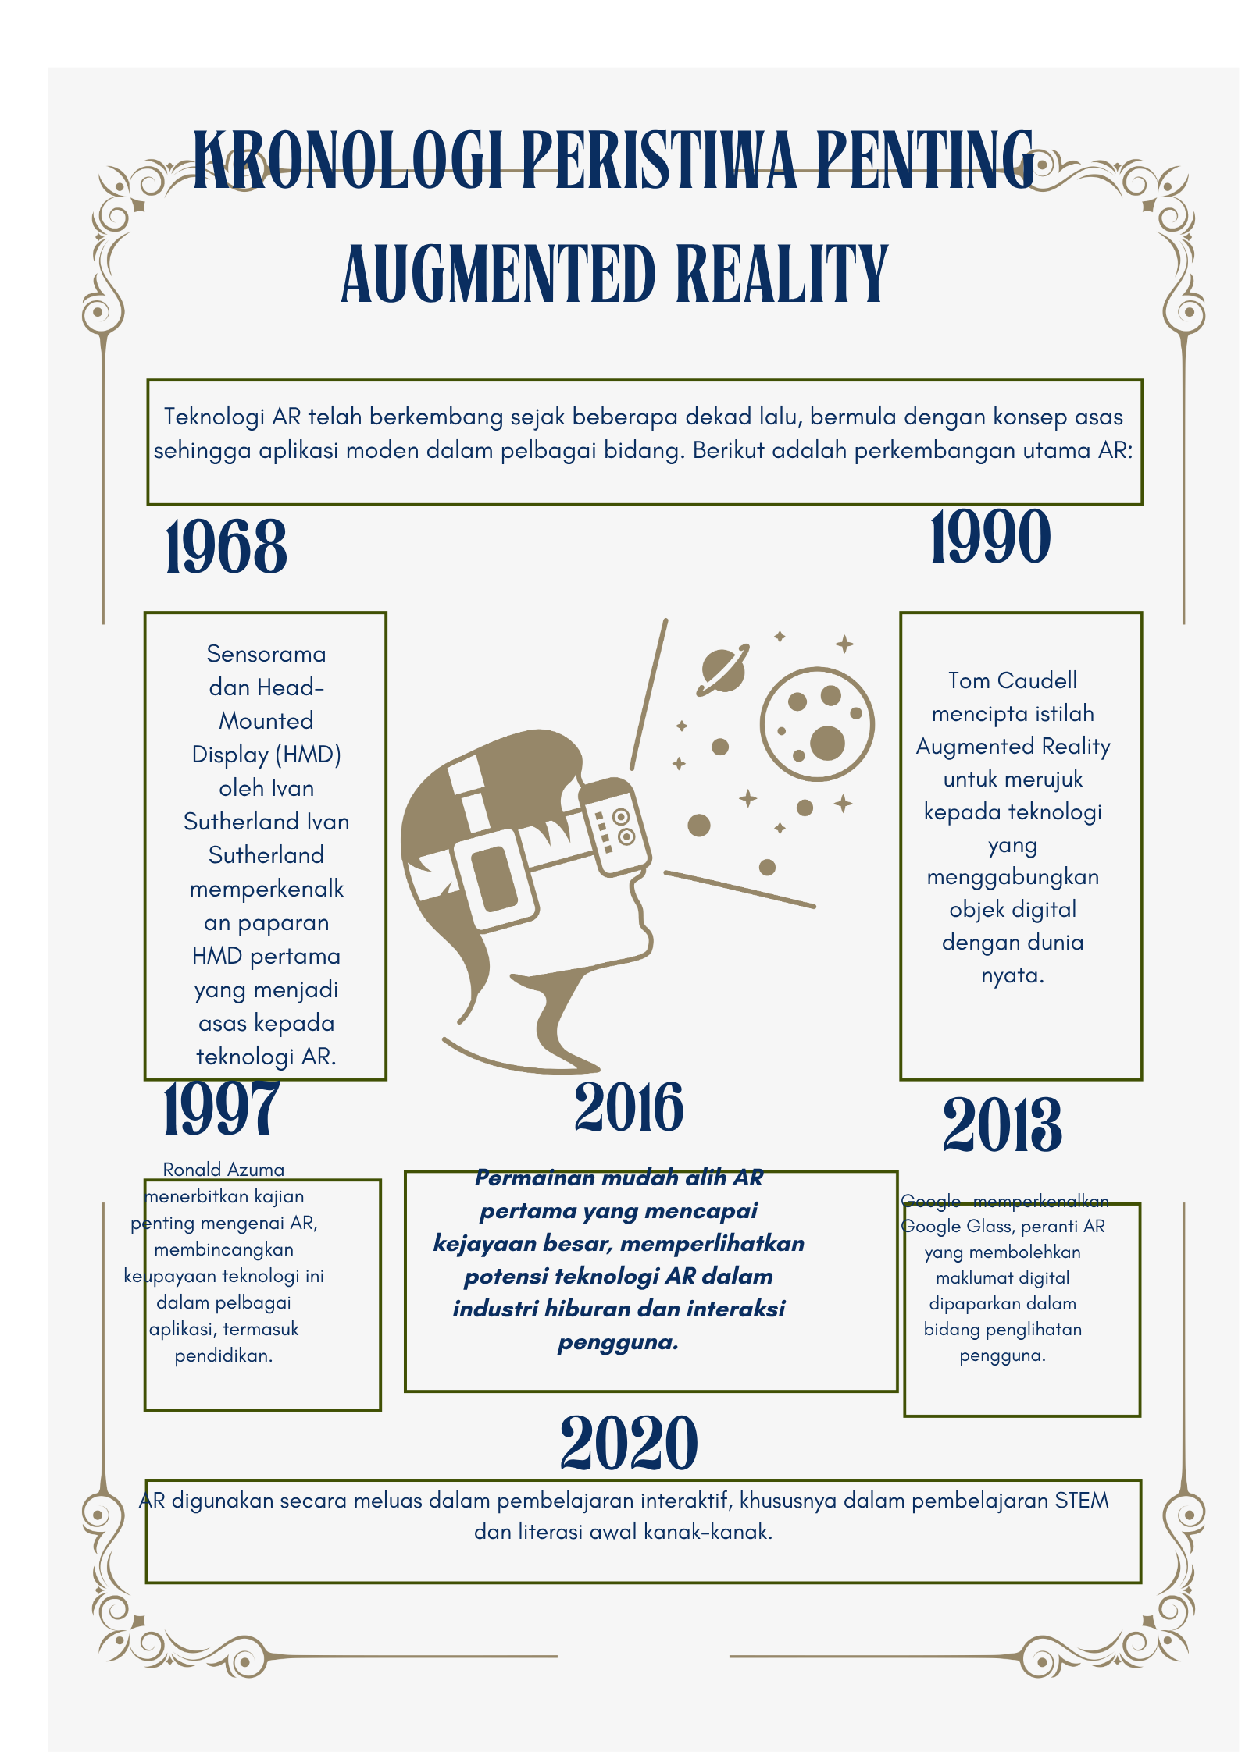
\includegraphics[width=1\linewidth]{info.pdf}
    \caption{Kronologi Peristiwa Penting Augmented Reality}
    \label{fig:enter-label}
\end{figure}
\begin{itemize}
    \item Meningkatkan pemahaman konsep abstrak melalui visualisasi 3D.
    \item Menggalakkan pembelajaran kendiri dengan akses kepada kandungan digital yang lebih menarik.
    \item Memudahkan guru menyampaikan konsep yang lebih sukar dengan lebih jelas.
    \item Meningkatkan motivasi dan daya ingatan pelajar melalui interaksi langsung dengan bahan pembelajaran.
\end{itemize}

Kajian menunjukkan bahawa AR boleh digunakan dalam pelbagai bidang pendidikan, termasuk sains, matematik, bahasa, dan sejarah.

\subsection{{Kajian Terdahulu mengenai AR dalam Pendidikan}}

Jadual 2.5 menunjukkan kajian terdahulu yang membincangkan kesan penggunaan AR dalam pendidikan:

\begin{table}[ht]
    \centering
    \caption{Jadual 2-5: Kajian Terdahulu Mengenai AR dalam Pendidikan}
    \begin{tabular}{@{}>{\raggedright\arraybackslash}p{7cm}>{\raggedright\arraybackslash}p{7cm}@{}}
        \toprule
        \textbf{Kajian} & \textbf{Hasil Kajian} \\
        \midrule
        Sehkar Fayda-Kinik (2023) & AR meningkatkan pemahaman dan motivasi pelajar. \\
        Yiannis Koumpouros (2024) & AR membantu pelajar memahami konsep dengan lebih mendalam. \\
        Lampropoulos et al. (2022) & AR meningkatkan penglibatan dan prestasi akademik pelajar. \\
        \bottomrule
    \end{tabular}
\end{table}

\subsection{Kajian lepas berkaitan penggunaan teknologi Augmented Reality (AR)}

Jadual~\ref{2.9} menunjukkan ringkasan sepuluh kajian lepas berkaitan penggunaan teknologi Augmented Reality (AR) dalam pendidikan sepanjang lima tahun terkini, khususnya dari segi impak terhadap motivasi, penumpuan, dan pencapaian pelajar.


\begin{table}[ht]
    \centering
    \caption{Ringkasan Dapatan Kajian Terkini}
    \begin{tabular}{cl>{\raggedright\arraybackslash}p{0.16\linewidth}>{\raggedright\arraybackslash}p{0.54\linewidth}}
        \toprule
        Bil & Tahun & Penulis & Dapatan \\
        \midrule
        1 & 2023 & Gunalan et al. & Meningkatkan motivasi dan tumpuan murid melalui visual interaktif dan aktiviti permainan. \\
        2 & 2022 & Lin et al. & Meningkatkan penumpuan dan pencapaian murid berbanding kaedah tradisional. \\
        3 & 2021 & Gunawan et al. & Meningkatkan motivasi intrinsik dan pencapaian ujian pelajar. \\
        4 & 2020 & Sánchez et al. & Meningkatkan tumpuan dan ingatan pelajar. \\
        5 & 2019 & Norazlina et al. & Peningkatan motivasi dan pencapaian murid dalam pengenalan huruf. \\
        6 & 2023 & Cao \& Yu & Sikap dan pencapaian lebih tinggi, tiada perbezaan signifikan motivasi. \\
        7 & 2025 & Ruijia et al. & Meningkatkan motivasi melalui pengalaman pembelajaran imersif. \\
        8 & 2023 & Özeren \& Top & Meningkatkan pencapaian akademik dan motivasi berbanding tradisional. \\
        9 & 2022 & Goharinejad et al. & Mengurangkan defisit perhatian dan meningkatkan pembelajaran. \\
        10 & 2023 & Vidak et al. & Membantu visualisasi konsep abstrak dan meningkatkan pencapaian pelajar. \\
        \bottomrule
    \end{tabular}
\end{table}

\section{\textbf{PERKEMBANGAN LITERASI AWAL KANAK-KANAK}}

Literasi awal merujuk kepada kebolehan asas kanak-kanak untuk mengenal huruf, memahami fonetik dan membina hubungan antara simbol dan bunyi.

\subsection{ Teknologi Dalam Pendidikan Prasekolah}

Dalam era Revolusi Industri 4.0, pendidikan prasekolah tidak terkecuali daripada menerima impak transformasi digital. Teknologi pendidikan telah diperkenalkan secara meluas di peringkat prasekolah.

\begin{table}[htbp]
    \centering
    \caption{Kajian Literatur mengenai Integrasi Augmented Reality (AR) dalam Pendidikan Bahasa}
    \begin{tabular}{p{4cm} p{10cm}}
        \toprule
        \textbf{Pengarang} & \textbf{Hasil Kajian} \\
        \midrule
        Ibrahim et al. (2018) & Teknologi AR menyediakan pengalaman pembelajaran imersif dan persekitaran pembelajaran yang menyeronokkan. \\
        Taskiran (2019) & Hasil soal selidik menunjukkan pembelajaran berasaskan AR lebih menyeronokkan dan memberi motivasi. \\
        Xu et al. (2019) & AR meningkatkan perhatian serta keterujaan pelajar dalam kelas ESL. \\
        Ji \& Shin (2019) & AR meningkatkan minat dan rasa ingin tahu pelajar, sekaligus memperkukuhkan motivasi dalam pembelajaran bahasa. \\
        Yaacob et al. (2019) & AR berkesan dalam meningkatkan pembelajaran kosa kata serta mengekalkan tahap motivasi yang tinggi. \\
        Chang et al. (2020) & Hasil kajian menunjukkan AR meningkatkan kepekatan, keyakinan, dan menyediakan senario pembelajaran yang hampir kepada realiti. \\
        Tsai (2020) & Pembelajaran kosa kata berasaskan AR lebih berkesan berbanding kaedah tradisional. \\
        Afnan et al. (2021) & Motivasi dan prestasi pelajar meningkat dengan penggunaan teknik pembelajaran berasaskan AR. \\
        Jalaluddin et al. (2021) & MAVR ialah alat interaktif yang berkesan dalam pembelajaran kosa kata Inggeris sebagai Bahasa Kedua (ESL). \\
        \bottomrule
  \end{tabular}
  \end{table}
\section*{2.6 Tumpuan, Pemahaman dan Motivasi Murid dalam Pembelajaran Berasaskan AR}

Keupayaan teknologi \textit{Augmented Reality} (AR) dalam merangsang perhatian dan motivasi pelajar telah menjadi fokus utama dalam pelbagai kajian terkini, khususnya dalam konteks pendidikan awal kanak-kanak. Sifat AR yang bersifat interaktif dan visual mampu meningkatkan daya tumpuan serta penglibatan kognitif murid semasa proses pembelajaran (Aydoğdu, 2021). Interaksi secara langsung dengan objek maya dalam persekitaran sebenar menjadikan pembelajaran lebih menyeronokkan dan membantu mengekalkan minat murid terhadap kandungan yang disampaikan.

\hspace{1cm}Kajian oleh Şener dan Kağıtçıbaşı (2024) menunjukkan bahawa aplikasi AR yang bersifat imersif memperkukuh motivasi intrinsik murid, terutamanya dalam situasi pembelajaran kendiri. Murid cenderung untuk lebih fokus apabila kandungan pembelajaran ditampilkan dalam bentuk visual tiga dimensi yang boleh diputar, dizum, dan disentuh secara maya. Keadaan ini meningkatkan tahap keseronokan dan keterlibatan murid dengan bahan pembelajaran.

\hspace{1cm}Dari aspek pemahaman, AR terbukti mampu membantu murid memahami kandungan dengan lebih mendalam. Kajian oleh Pan et al. (2021) menunjukkan bahawa penggunaan AR dalam aktiviti penceritaan secara digital meningkatkan pemahaman cerita serta kebolehan menyusun semula peristiwa mengikut urutan yang betul. Tambahan pula, kajian oleh Frontiers in Psychology (2024) mendapati bahawa murid yang menggunakan \textit{AR storybooks} memperoleh skor lebih tinggi dalam penilaian kefahaman berbanding murid yang menggunakan buku cerita biasa.

\hspace{1cm}Selain itu, kajian terkini oleh Springer (2024) meneliti hubungan antara tempoh pendedahan AR dengan pencapaian pemahaman. Dapatan menunjukkan bahawa penggunaan AR secara sederhana (24–39 saat per interaksi) memberi kesan yang lebih efektif terhadap pemahaman berbanding pendedahan terlalu pendek (11–13 saat), sekali gus mengurangkan beban kognitif murid.

\hspace{1cm}Motivasi belajar juga dilihat meningkat secara signifikan dalam kalangan murid prasekolah apabila pendekatan AR digunakan dalam pembelajaran literasi. Kajian oleh Lim dan Goh (2021) serta Rahman et al. (2022) mendapati bahawa aplikasi fonik berasaskan AR bukan sahaja meningkatkan motivasi dan daya tumpuan murid, malah turut menyumbang kepada penguasaan fonemik dan abjad dengan lebih pantas.

\hspace{1cm}Kesemua dapatan ini sejajar dengan prinsip dalam rangka kerja \textit{Concept-Oriented Reading Instruction} (CORI) yang menekankan integrasi strategi pembelajaran dan elemen motivasi seperti \textit{self-efficacy}, \textit{intrinsic motivation} dan \textit{autonomy support} untuk menghasilkan pemahaman membaca yang lebih baik (Guthrie \& Wigfield, 2016).

\hspace{1cm}Secara keseluruhannya, pelaksanaan teknologi AR dalam pendidikan awal berupaya memberi kesan positif yang signifikan terhadap tumpuan, motivasi serta pemahaman murid. Ciri-ciri unik AR seperti visualisasi interaktif, maklum balas masa nyata dan pelibatan deria pelbagai membolehkan kanak-kanak belajar dengan lebih aktif, menyeronokkan dan berkesan.


\section{Model ADDIE}

Rajah Menunjukkan Modeal ADDIE yang digunakan dalam kajian ini.
\begin{figure}[h]
    \centering
    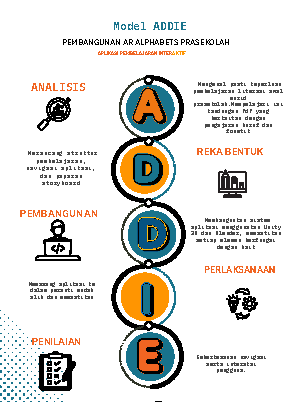
\includegraphics[width=1\linewidth]{MODEL ADDIES.pdf}
    \caption{Model ADDIE}
    \label{fig:enter-addie}
\end{figure}




\section{Unity }
Unity 3D adalah perisian untuk mencipta permainan tiga dimensi yang 
digabungkan untuk menghasilkan animasi tiga dimensi secara masa nyata 
(waktu nyata). Unity dilengkapi dengan Persekitaran Pembangunan Terpadu (IDE) 
dikenali sebagai Mono Develop, yang bertujuan untuk mengintegrasikan semua skrip 
dihasilkan ke dalam Unity, untuk diproses secara langsung. Unity 3D 
dibangunkan oleh Unity Technologies, ditubuhkan pada tahun 2004 oleh David 
Helgason, Nicholas Francis, dan Joachim Ante. Pada tahun 2009, Unity dilancarkan 
secara percuma, dan kini ia telah menarik berjuta-juta pembangun dari seluruh dunia 
untuk mendaftar (Rahmat & Yanti, 2021). Unity menyokong pembangunan aplikasi 
Android. Sebelum aplikasi yang dibina menggunakan Unity untuk Android 
boleh dijalankan, konfigurasi persekitaran pembangunan Android pada peranti adalah  diperlukan. Untuk itu, pembangun perlu memuat turun dan memasang Android SDK.  dan menambah peranti fizikal ke dalam sistem. Unity Android membenarkan memanggil fungsi khas yang ditulis dalam C/C++ secara langsung dan Java secara tidak langsung secara tidak langsung melalui skrip C# (Andriansyah et al., 2019).

\section{Blender}
Software	Description
	Unity 3D adalah perisian untuk mencipta permainan tiga dimensi yang 
digabungkan untuk menghasilkan animasi tiga dimensi secara masa nyata 
(waktu nyata). Unity dilengkapi dengan Persekitaran Pembangunan Terpadu (IDE) 
dikenali sebagai Mono Develop, yang bertujuan untuk mengintegrasikan semua skrip 
dihasilkan ke dalam Unity, untuk diproses secara langsung. Unity 3D 
dibangunkan oleh Unity Technologies, ditubuhkan pada tahun 2004 oleh David 
Helgason, Nicholas Francis, dan Joachim Ante. Pada tahun 2009, Unity dilancarkan 
secara percuma, dan kini ia telah menarik berjuta-juta pembangun dari seluruh dunia 
untuk mendaftar (Rahmat & Yanti, 2021). Unity menyokong pembangunan aplikasi 
Android. Sebelum aplikasi yang dibina menggunakan Unity untuk Android 
boleh dijalankan, konfigurasi persekitaran pembangunan Android pada peranti adalah  diperlukan. Untuk itu, pembangun perlu memuat turun dan memasang Android SDK.  dan menambah peranti fizikal ke dalam sistem. Unity Android membenarkan memanggil fungsi khas yang ditulis dalam C/C++ secara langsung dan Java secara tidak langsung secara tidak langsung melalui skrip C# (Andriansyah et al., 2019).

	\hspace{1cm}Blender merupakan salah satu perisian percuma yang sering dikenali sebagai suite penciptaan 3D sumber terbuka, yang menyokong keseluruhan proses dalam mod tiga dimensi seperti pemodelan, pemasangan rangka, animasi, simulasi, rendering, dan penjejakan gerakan. Malah, perisian ini juga menyokong pembangunan permainan (Valentino, 2017). Pada mulanya, Blender diciptakan sebagai alat pengeluaran dalaman untuk syarikat animasi Belanda yang terkemuka, NeoGeo, yang diasaskan oleh pemaju asal Blender dan masih menjadi pemaju utama hingga ke hari ini, Ton Roosendaal. Menjelang akhir tahun 1990-an, NeoGeo mula menawarkan salinan Blender untuk dimuat turun melalui laman web mereka. Secara perlahan tetapi konsisten, minat terhadap program yang kurang daripada 2 MB ini semakin berkembang. Pada tahun 1998, Ton menubuhkan syarikat baharu, Not a Number (NaN), untuk memasarkan dan menjual Blender sebagai produk perisian. NaN terus menyediakan versi percuma Blender tetapi juga menawarkan versi premium dengan lebih banyak ciri pada harga yang berpatutan. Strategi ini terbukti berkesan, dan pada akhir tahun 2000, pengguna Blender telah mencapai lebih daripada 250,000 di seluruh dunia (Gumster, 2015, hal. 11).
\section{Vuforia}
	Vuforia adalah Kit Pembangunan Perisian (SDK) yang dibangunkan oleh Qualcomm untuk membantu pembangun aplikasi mudah alih dalam mencipta aplikasi Realiti Terimbuh (AR) pada telefon pintar sama ada berasaskan Android atau iOS (Rahmat & Yanti, 2021). SDK Vuforia juga boleh diintegrasikan dengan Unity, dikenali sebagai Vuforia AR Extension for Unity. Vuforia AR Extension membolehkan Unity memaparkan animasi realiti terimbuh yang telah direka sebelumnya (Desierto et al., 2020). Untuk berfungsi dengan optimum, SDK Vuforia memerlukan beberapa komponen penting. Komponen tersebut merangkumi kamera, penukar imej, alat pengesan, rendering latar belakang video, kod aplikasi, trackables, dan marker. Semua komponen ini digunakan dalam pembangunan aplikasi berasaskan AR (Mustaqim, 2017).
\section{Figma}
	Figma merupakan salah satu alat reka bentuk yang sering digunakan untuk mencipta antaramuka aplikasi mudah alih, desktop, laman web, dan banyak lagi. Figma boleh diakses pada sistem operasi Windows, Linux, atau Mac dengan sambungan internet. Keunggulan Figma terletak pada kemampuannya untuk membolehkan lebih dari satu individu berkolaborasi secara serentak, walaupun berada di lokasi yang berbeza. Fenomena ini dapat dianggap sebagai kerja berkumpulan, dan disebabkan oleh keupayaan aplikasi Figma, ia telah menjadi pilihan utama bagi banyak pereka UI/UX untuk menghasilkan prototaip laman web atau aplikasi dengan cara yang cepat dan berkesan (Al-Faruq et al., 2022).
	Adobe Illustrator merupakan aplikasi yang digunakan untuk menyunting reka bentuk grafik dalam penerbitan web dan desktop, serta mampu berintegrasi dengan perisian lain yang relevan (Rian et al., 2021). Adobe Illustrator dapat digunakan untuk menyunting atau mencipta imej dan butang dalam proses pembangunan aplikasi.


\begin{tabular}{>{\raggedright}p{3cm}>{\centering}p{2cm}p{8cm}}
\toprule
\textbf{Aplikasi AR} & \textbf{Logo} & \textbf{Huraian} \\
\midrule
Dinosaur3DAR & 

\includegraphics[width=1.5cm]{dino.pdf}& 
Aplikasi ini dikhuskan kepada penggemar dinosaur.  Aplikasi ini amat sesuai untuk kanak-kanak yang teruja menerokai dunia prasejarah dan mempelajari tentang makhluk purba seperti dinosaur.\\

Earth Zoo AR & 

\includegraphics[width=1.5cm]{===200.pdf}& 
 menampilkan objek dalam bentuk 3D. EarthZoo-AR menawarkan pengalaman seolah-olah melawat zoo maya.\\

Kad Flash AR & 

\includegraphics[width=1.5cm]{===300.pdf}& 
Aplikasi ini bertujuan untuk mendidik kanak-kanak melalui kad flash AR. Dengan pemanfaatan teknologi ini, kanak-kanak dapat melihat huruf dan haiwan dalam bentuk 3D sambil mendengar nama serta bunyi haiwan tersebut, m\\

Math ARi & 

\includegraphics[width=1.5cm]{mate.pdf} & 
Aplikasi ini direka untuk memperkenalkan kanak-kanak kepada asas-asas pembelajaran seperti huruf, nama haiwan, dan kata-kata melalui interaksi AR yang menghiburkan. Ia amat sesuai untuk kanak-kanak kecil kerana pendekatannya yang mudah dan berkesan. \\

AR Paint & 

\includegraphics[width=1.5cm]{zooz1.pdf}& 
Aplikasi kreatif ini membolehkan pengguna menghasilkan hologram 3D, lukisan, dan patung. Ia menawarkan peluang untuk meneroka kreativiti, menyertai komuniti seni maya.\\
\bottomrule
\end{tabular}

\subsection{2.6 Penggunaan UML dalam Pembangunan Aplikasi Pendidikan AR}

Pembangunan aplikasi pendidikan seperti \textit{AR Alphabets} memerlukan perancangan yang sistematik, terutamanya dari aspek kejuruteraan perisian. Salah satu pendekatan yang digunakan ialah penggunaan Unified Modeling Language (UML) bagi memvisualisasikan keperluan sistem dan interaksi antara pengguna dengan sistem. UML membantu dalam dokumentasi proses pembangunan aplikasi, menjadikan reka bentuk lebih jelas dan mudah difahami oleh pembangun.

Dalam konteks aplikasi \textit{AR Alphabets}, beberapa jenis diagram UML telah digunakan:
\begin{itemize}
  \item \textbf{Use Case Diagram} – menunjukkan fungsi sistem dan peranan pengguna.
  \item \textbf{Activity Diagram} – menerangkan urutan aktiviti pengguna semasa menggunakan fungsi tertentu dalam aplikasi.
  \item \textbf{Flowchart} – memvisualisasikan aliran proses untuk setiap modul aplikasi.
\end{itemize}

Rajah-rajah berikut menunjukkan contoh diagram UML yang digunakan dalam aplikasi ini.


\subsection{Teori Tindakan Norman dalam Reka Bentuk Antaramuka Pengguna}

Teori Tindakan oleh Donald Norman (1990) merupakan salah satu teori asas dalam bidang interaksi manusia-komputer (HCI) yang menjelaskan proses mental dan tindakan fizikal yang berlaku apabila pengguna berinteraksi dengan sesuatu sistem atau aplikasi. Teori ini terdiri daripada tujuh peringkat, iaitu: (i) penetapan matlamat (forming the goal), (ii) penetapan niat (forming the intention), (iii) penentuan tindakan (specifying an action), (iv) pelaksanaan tindakan (executing the action), (v) persepsi kesan (perceiving the system state), (vi) pentafsiran kesan (interpreting the system state), dan (vii) penilaian hasil (evaluating the outcome)norman1990}.

Dalam konteks pembangunan aplikasi \textit{AR Alphabets}, teori ini memainkan peranan penting dalam memastikan reka bentuk antaramuka adalah selaras dengan jangkaan dan keperluan pengguna, khususnya murid prasekolah dan guru. Sebagai contoh, apabila murid ingin mengenali huruf, mereka mempunyai matlamat (mengenal huruf), kemudian menetapkan niat (menekan kad AR atau ikon huruf), melaksanakan tindakan tersebut, dan aplikasi akan memberikan maklum balas visual dan audio. Sekiranya aplikasi berjaya membantu murid mencapai matlamat ini dengan mudah, maka jurang tindakan (gulf of execution) dan jurang penilaian (gulf of evaluation) dapat dikurangkan.

\textbf{Jurang Tindakan (Gulf of Execution)} merujuk kepada kesukaran pengguna untuk melaksanakan tindakan yang sesuai dalam sistem. Dalam aplikasi \textit{AR Alphabets}, antaramuka yang intuitif, susunan ikon yang jelas, dan interaksi berasaskan sentuhan membantu murid prasekolah melaksanakan tindakan mereka dengan lebih mudah tanpa kekeliruan.

\textbf{Jurang Penilaian (Gulf of Evaluation)} pula merujuk kepada kesukaran pengguna memahami kesan tindakan mereka. Aplikasi ini meminimumkan jurang tersebut melalui maklum balas segera seperti animasi 3D, bunyi fonetik, dan paparan visual yang menyatakan huruf yang sedang dipelajari. Murid dapat segera menilai bahawa tindakan mereka (menekan butang atau mengimbas kad) telah menghasilkan tindak balas yang tepat.
\subsection{Hubungan Teori Norman dengan Skala SUS dalam Kajian Ini}

Dalam kajian ini, tahap kebolehgunaan aplikasi telah dinilai menggunakan \textit{System Usability Scale (SUS)}, yang mengukur aspek kejelasan, keberkesanan, dan kepuasan pengguna terhadap sistem. Dapatan skor SUS sebanyak 87.5 menunjukkan bahawa aplikasi \textit{AR Alphabets} berada pada tahap kebolehgunaan yang sangat baik.

Teori Norman memperkukuh dapatan ini dengan menjelaskan mengapa aplikasi ini berfungsi dengan baik dari perspektif interaksi pengguna. Reka bentuk antaramuka yang meminimumkan beban kognitif dan membolehkan pengguna mencapai matlamat mereka dengan mudah adalah faktor utama yang menyumbang kepada skor SUS yang tinggi. Dengan kata lain, apabila jurang tindakan dan penilaian dapat diminimumkan melalui reka bentuk sistem yang sesuai, pengguna lebih cenderung untuk berasa puas, memahami fungsi sistem, dan menggunakannya dengan cekap—sejajar dengan elemen-elemen yang diukur dalam SUS.

\begin{figure}[H]
\centering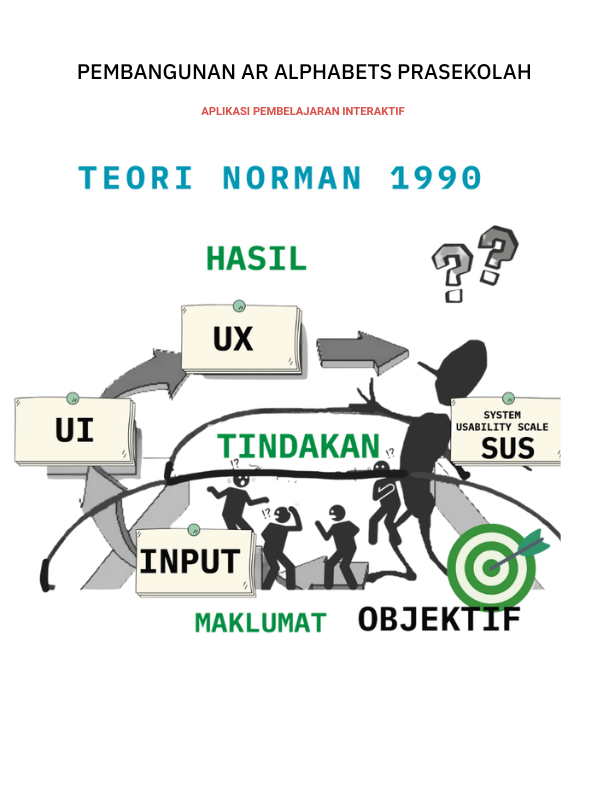
\includegraphics[width=0.8\textwidth]{------norman teori.png}\caption{Model Tindakan Norman dalam Konteks Aplikasi \textit{AR Alphabets} (Disesuaikan daripada Norman, 1990)}\label{rajah:norman}\end{figure}

\subsection{Skala Kebolehgunaan Sistem (System Usability Scale, SUS)}

Dalam usaha menilai sejauh mana kejayaan sesuatu sistem atau aplikasi, satu bentuk pengukuran yang kerap digunakan ialah Skala Kebolehgunaan Sistem atau \textit{System Usability Scale} (SUS). SUS merupakan satu instrumen soal selidik yang dibangunkan oleh John Brooke pada tahun 1986 bagi menilai aspek kebolehgunaan pelbagai jenis produk dan sistem termasuk aplikasi mudah alih, laman sesawang, dan perisian interaktif (brooke, 1986).

Terdapat beberapa ciri unik SUS yang menjadikannya salah satu alat penilaian yang paling popular dan praktikal dalam kajian pengalaman pengguna. Pertama, SUS hanya terdiri daripada sepuluh item soalan, menjadikannya mudah dan cepat untuk dijawab oleh responden {Kedua, SUS bersifat agnostik teknologi, membolehkannya digunakan untuk menilai hampir semua jenis antara muka seperti laman sesawang, aplikasi telefon pintar, sistem maklum balas suara (IVR), sistem berasaskan sentuhan, dan lain-lain . Ketiga, hasil soal selidik ini dikira menjadi satu skor tunggal antara 0 hingga 100, yang mudah difahami oleh pengguna dari pelbagai latar belakang teknikal mahupun bukan teknikal (brooke, 1986).

\begin{figure}[H]   
\centering    \includegraphics[width=0.8\textwidth]{Screenshot 2025-07-05 at 1.16.03 AM.png}    \caption{Skor SUS Berdasarkan Kategori Penilaian \cite{bangor2009determining}}    \label{fig:sus-score}\end{figure}

Skor SUS yang diperoleh biasanya ditafsir mengikut julat berikut:

\begin{itemize}    \item \textbf{Grade A (Sangat Baik)}: Skor $\geq$ 84    \item \textbf{Grade B (Baik)}: Skor antara 72 hingga kurang daripada 84    \item \textbf{Grade C (Memuaskan)}: Skor antara 53 hingga kurang daripada 72    \item \textbf{Grade D (Kurang Memuaskan)}: Skor antara 39 hingga kurang daripada 53    \item \textbf{Grade F (Tidak Memuaskan)}: Skor $<$ 39\end{itemize}

Melalui analisis SUS, penyelidik dapat menilai secara kuantitatif tahap kebolehgunaan sistem serta mengenal pasti keperluan penambahbaikan dalam reka bentuk antara muka pengguna.

Kesimpulannya, integrasi Teori Tindakan Norman dalam reka bentuk \textit{AR Alphabets} bukan sahaja memperkukuh aspek reka bentuk antaramuka, malah menyokong justifikasi keberkesanan aplikasi berdasarkan dapatan ujian SUS. Ia menjadikan pengalaman pengguna lebih intuitif dan bermakna, terutama bagi murid prasekolah yang memerlukan pembelajaran yang menyeronokkan serta mudah difahami.
\chapter{Methodologi Kajian}n 
\section{Pengenalan}

Bab ini membincangkan metodologi penyelidikan yang digunakan dalam pembangunan aplikasi \textit{AR Alphabets Prasekolah}. Metodologi penyelidikan merujuk kepada pendekatan sistematik yang digunakan oleh penyelidik untuk memperoleh data dan maklumat bagi mencapai objektif kajian (Ismail et al., 2021; Rahman & Zulkifli, 2023). 

Kajian ini menggunakan pendekatan Kajian Reka Bentuk dan Pembangunan (Design and Development Research, DDR) yang sesuai untuk pembangunan aplikasi pendidikan interaktif. Pendekatan ini membolehkan penyelidik membangunkan produk berasaskan keperluan pengguna sebenar serta menilai keberkesanannya secara sistematik (Kamaruddin et al., 2022). 

Bab ini turut menghuraikan reka bentuk kajian, prosedur pelaksanaan, kaedah persampelan, instrumen kajian, kaedah pengumpulan dan analisis data, serta langkah-langkah untuk memastikan kesahan dan kebolehpercayaan kajian mengikut struktur fasa DDR yang dilaksanakan.
\section{Reka Bentuk Kajian}

Kajian ini menggunakan pendekatan Reka Bentuk dan Pembangunan (Design and Development Research, DDR) yang merangkumi kaedah kuantitatif dan kualitatif mengikut fasa pelaksanaan. Kaedah kuantitatif digunakan dalam bentuk soal selidik untuk mengumpul data daripada responden, manakala kaedah kualitatif dilaksanakan melalui temu bual separa berstruktur. Kaedah tinjauan membolehkan data dikumpul dengan pantas dan berkesan, terutamanya apabila melibatkan pelbagai pembolehubah yang boleh dianalisis secara statistik (Zulkifli et al., 2021; Hassan & Rahim, 2022).

Secara keseluruhan, kajian ini berasaskan pendekatan DDR seperti yang digariskan oleh Richey dan Klein (2020), yang sesuai digunakan dalam pembangunan aplikasi pendidikan interaktif seperti \textit{AR Alphabets Prasekolah}. Pendekatan ini membolehkan penyelidik menambah baik proses pembelajaran melalui pembangunan produk yang berasaskan keperluan pengguna sebenar, serta menilai kebolehgunaan aplikasi secara praktikal dan sistematik. DDR juga dikenali sebagai kajian pembangunan (developmental research).

Menurut Richey dan Klein (2020), pendekatan DDR terdiri daripada tiga fasa utama yang sistematik, iaitu:
\begin{itemize}
  \item \textbf{Fasa 1: Analisis Keperluan} – Mengenal pasti keperluan pengguna terhadap aplikasi AR dalam konteks pembelajaran huruf prasekolah.
  \item \textbf{Fasa 2: Reka Bentuk dan Pembangunan} – Membangunkan aplikasi berdasarkan dapatan pakar dan keperluan pengguna menggunakan teknologi seperti Unity3D dan Vuforia SDK.
  \item \textbf{Fasa 3: Penilaian Kepenggunaan} – Menilai kefahaman, minat dan kebolehgunaan aplikasi melalui pemerhatian dan temu bual bersama murid prasekolah.
\end{itemize}

Pendekatan ini membolehkan penyelidik mengaplikasikan pelbagai instrumen dan teknik pengumpulan data secara sistematik mengikut keperluan setiap fasa. Oleh itu, kajian ini dikendalikan secara berperingkat mengikut ketiga-tiga fasa utama DDR yang saling melengkapi.
Kajian ini dilaksanakan melalui tiga fasa utama seperti yang digariskan dalam pendekatan DDR oleh Richey dan Klein (2020). Setiap fasa memainkan peranan penting dalam memastikan pembangunan aplikasi \textit{AR Alphabets Prasekolah} dijalankan secara sistematik dan berasaskan keperluan sebenar pengguna. Fasa-fasa tersebut adalah seperti berikut:

\begin{itemize}
  \item \textbf{Fasa 1: Analisis Keperluan} – Fasa ini bertujuan untuk mengenal pasti keperluan pengguna terhadap aplikasi AR dalam konteks pembelajaran huruf prasekolah. Data dikumpul melalui soal selidik dan temu bual bersama guru prasekolah.
  
  \item \textbf{Fasa 2: Reka Bentuk dan Pembangunan} – Fasa utama kajian ini melibatkan pembangunan aplikasi berdasarkan dapatan fasa pertama. Teknik Fuzzy Delphi digunakan untuk mendapatkan kesepakatan pakar dalam menentukan elemen penting yang perlu dimasukkan ke dalam aplikasi.
  
  \item \textbf{Fasa 3: Penilaian Kepenggunaan} – Fasa terakhir ini menilai kebolehgunaan aplikasi melalui temu bual dan pemerhatian terhadap murid prasekolah. Penilaian ini memberi gambaran tentang kefahaman, minat, dan keberkesanan aplikasi dalam menyampaikan kandungan pembelajaran.
\end{itemize}

Secara ringkasnya, kajian ini dijalankan mengikut tiga fasa utama DDR, iaitu analisis keperluan, reka bentuk dan pembangunan, serta penilaian kepenggunaan. Jadual~\ref{jadual:kaedahDDR} menunjukkan ringkasan kaedah kajian yang dijalankan berdasarkan setiap fasa, yang diadaptasikan daripada buku \textit{Design and Developmental Research: Emergent Trends in Educational Research} (Richey \& Klein, 2020).
\section{Kerangka Prosedur Kajian}

Bagi memastikan kajian ini dilaksanakan secara teratur dan sistematik, satu kerangka prosedur telah dibina untuk menggambarkan aliran pelaksanaan kajian berdasarkan pendekatan Reka Bentuk dan Pembangunan (Design and Development Research, DDR). Kajian ini dibahagikan kepada tiga fasa utama, iaitu fasa analisis keperluan, fasa reka bentuk dan pembangunan aplikasi, serta fasa penilaian kepenggunaan aplikasi. Aliran pelaksanaan kajian ini ditunjukkan dalam Rajah~\ref{rajah:prosedurKajian}.

\begin{table}[H]
\centering
\caption{Kaedah Kajian Mengikut Fasa DDR}
\label{jadual:kaedahDDR}
\begin{tabular}{|p{4cm}|p{10cm}|}
\hline
\textbf{Fasa Kajian} & \textbf{Kaedah yang Digunakan} \\
\hline
Fasa 1: Analisis Keperluan & Soal selidik untuk mengenal pasti keperluan pengguna terhadap aplikasi AR. Analisis data dilakukan berdasarkan skor min dan peratusan. \\
\hline
Fasa 2: Reka Bentuk dan Pembangunan Aplikasi & Kajian literatur dan kaedah Fuzzy Delphi digunakan untuk mendapatkan kesepakatan pakar dalam menentukan elemen penting aplikasi. \\
\hline
Fasa 3: Penilaian Kepenggunaan Aplikasi & Temu bual separa berstruktur dijalankan bersama murid dan guru prasekolah untuk menilai kefahaman, minat dan kebolehgunaan aplikasi. \\
\hline
\end{tabular}
\end{table}
\section{Fasa-fasa dalam Kajian}

Kajian ini dilaksanakan mengikut tiga fasa utama berdasarkan pendekatan Reka Bentuk dan Pembangunan (DDR), iaitu fasa analisis keperluan (fasa satu), fasa reka bentuk dan pembangunan aplikasi (fasa dua), dan fasa penilaian kepenggunaan aplikasi (fasa tiga). Setiap fasa memainkan peranan penting dalam memastikan pembangunan aplikasi \textit{AR Alphabets Prasekolah} dijalankan secara sistematik dan berasaskan keperluan sebenar pengguna.

\subsection{Fasa 1: Analisis Keperluan}

Fasa pertama dalam pendekatan DDR ialah fasa analisis keperluan. Fasa ini amat penting kerana ia membantu penyelidik mengenal pasti persoalan kajian dan keperluan pengguna sasaran sebelum pembangunan aplikasi dijalankan (Ridhuan et al., 2014). Dalam konteks kajian ini, fasa ini bertujuan untuk mengenal pasti keperluan murid dan guru prasekolah terhadap aplikasi pembelajaran berasaskan realiti terimbuh (AR) bagi topik pengenalan huruf.

Menurut McKillip (1987), analisis keperluan melibatkan proses mengenal pasti dan menilai keperluan sesuatu perkara yang akan menentukan hala tuju penyelesaian. Proses ini juga dikenali sebagai proses mengenal pasti masalah dalam kalangan populasi sasaran (target population), serta mengenal pasti pendekatan terbaik untuk menyelesaikan masalah tersebut (Witkin \& Altschuld, 1995). Riviere (1996) menegaskan bahawa analisis keperluan lebih memfokuskan kepada apa yang sepatutnya berlaku (what ought to be) berbanding apa yang sedang berlaku (what is).

McKillip (1987) turut mencadangkan beberapa model yang bolehModel ini menekankan tiga komponen utama. Pertama, proses menetapkan apa yang sepatutnya dilakukan. Kedua, proses pengukuran prestasi semasa. Ketiga, proses mengenal pasti ketidaksesuaian (discrepancy identification), iaitu jurang antara apa yang sepatutnya berlaku (\textit{what ought to be}) dengan apa yang sedang berlaku (\textit{what is}).

\item \textbf{Model Pemasaran (Marketing Model)} – Model ini memberi tumpuan kepada proses menganalisis keperluan dan maklum balas pengguna bagi menilai perkara yang diperlukan dalam sesuatu perkhidmatan atau produk. Dalam konteks pendidikan, model ini sesuai digunakan untuk mengenal pasti keperluan pengguna sasaran seperti guru dan murid. Terdapat tiga komponen utama dalam model ini:

\begin{itemize}
  \item \textbf{Pemilihan populasi sasaran} – Melibatkan pemilihan kumpulan pengguna yang berpotensi tinggi untuk menggunakan produk atau perkhidmatan yang dibangunkan.
  \item \textbf{Pengkuantitian (quantification)} – Proses mengukur dan menilai keperluan pengguna serta menganalisis nilai dan minat mereka terhadap produk.
  \item \textbf{Sintesis (synthesis)} – Penyediaan indeks keperluan yang memberi gambaran menyeluruh tentang keperluan sebenar pengguna dan maklumat berkaitan produk yang dicadangkan.
\end{itemize}
Namun demikian, berdasarkan ketiga-tiga model yang dibincangkan, penyelidik memilih untuk menggunakan Model Ketidaksesuaian (Discrepancy Model) sebagai model pendukung dalam fasa analisis keperluan.

Penyelidik menggunakan teknik soal selidik dan temu bual untuk menilai sejauh mana keperluan terhadap pembangunan aplikasi \textit{AR Alphabets Prasekolah}. Pandangan guru prasekolah dan pakar pendidikan awal kanak-kanak dijadikan asas dalam mengenal pasti keperluan pengguna. Dapatan yang diperoleh daripada fasa ini digunakan sebagai asas untuk mereka bentuk aplikasi yang bersesuaian dengan konteks pembelajaran huruf bagi murid prasekolah.

Dalam aspek analisis keperluan ini, penyelidik menggariskan prosedur berikut:

\begin{itemize}
  \item Mengenal pasti kumpulan sasaran yang terdiri daripada guru dan murid prasekolah.
  \item Menjalankan soal selidik kepada 50 responden untuk mengenal pasti keperluan pengguna terhadap aplikasi pembelajaran huruf berasaskan AR.
  \item Menjalankan temu bual bersama dua orang pakar pendidikan awal kanak-kanak untuk mendapatkan pandangan profesional.
\end{itemize}

\subsubsection{Soal Selidik untuk Fasa Analisis Keperluan}

Fasa ini memfokuskan kepada keperluan murid dan guru prasekolah terhadap aplikasi pembelajaran huruf menggunakan teknologi realiti terimbuh. Seramai 50 responden terlibat dalam soal selidik ini, terdiri daripada ibu bapa dan guru yang mewakili pengguna sasaran aplikasi. Soal selidik ini direka bentuk untuk mengenal pasti tahap pendedahan terhadap teknologi, keperluan pembelajaran literasi awal, serta kesediaan menggunakan aplikasi AR dalam konteks prasekolah.

Responden yang terlibat dalam fasa ini diringkaskan dalam Jadual~\ref{jadual:respondenAnalisis}.
\begin{table}[H]
\centering
\caption{Responden Kajian Fasa Satu (Analisis Keperluan)}
\label{jadual:respondenAnalisis}
\begin{tabular}{|p{6cm}|c|}
\hline
\textbf{Responden Kajian} & \textbf{Jumlah} \\
\hline
Guru Prasekolah Zon Bangsar & 20 \\
\hline
Guru Prasekolah Zon Keramat & 15 \\
\hline
Guru Prasekolah Zon Sentul & 15 \\
\hline
\textbf{Jumlah Responden} & \textbf{50 orang} \\
\hline
\end{tabular}
\end{table}
\subsubsection{Instrumen Kajian Fasa Analisis Keperluan}

Instrumen soal selidik digunakan dalam fasa pertama kajian untuk mendapatkan maklum balas berkaitan keperluan terhadap pembangunan aplikasi \textit{AR Alphabets Prasekolah}. Soal selidik ini dibina secara berstruktur dan diubah suai berdasarkan instrumen kajian terdahulu seperti kajian reka bentuk modul m-Pembelajaran Bahasa Arab oleh Amani Dahaman (2014) dan kajian m-Pembelajaran di sekolah menengah oleh Ahmad Sobri (2010).

Soal selidik ini terdiri daripada empat bahagian utama:

\begin{itemize}
  \item \textbf{Bahagian I: Maklumat Demografi} – Mengumpul maklumat latar belakang responden seperti umur, pengalaman mengajar, dan tahap pendedahan terhadap teknologi.
  \item \textbf{Bahagian II: Penggunaan Teknologi Mudah Alih} – Mengandungi item berskala Likert lima mata: (1) Sangat Tidak Kerap, (2) Tidak Kerap, (3) Tidak Pasti, (4) Kerap, dan (5) Sangat Kerap.
  \item \textbf{Bahagian III, IV dan V: Persepsi terhadap Aplikasi AR} – Mengandungi item berskala Likert lima mata: (1) Sangat Tidak Setuju, (2) Tidak Setuju, (3) Tidak Pasti, (4) Setuju, dan (5) Sangat Setuju. Bahagian ini merangkumi aspek keperluan aplikasi, reka bentuk kandungan, dan kesesuaian teori pembelajaran.
\end{itemize}

Ringkasan pembinaan instrumen soal selidik bagi fasa analisis keperluan ditunjukkan dalam Jadual~\ref{jadual:instrumenAnalisis}.
\begin{table}[h]
\centering
\caption{Ringkasan Pembinaan Instrumen Fasa Analisis Keperluan}
\label{jadual:instrumenAnalisis}
\begin{tabular}{|p{6cm}|p{5cm}|c|}
\hline
\textbf{Item / Pembolehubah} & \textbf{Sumber Rujukan} & \textbf{Bilangan Item} \\
\hline
Penggunaan Teknologi Mudah Alih & Ahmad Sobri (2010) & 10 \\
\hline
Pengetahuan tentang Aplikasi AR & Ahmad Sobri (2010) & 12 \\
\hline
Reka Bentuk Kandungan Aplikasi & Amani Dahaman (2014) & 13 \\
\hline
Strategi Pengajaran dan Pembelajaran & Amani Dahaman (2014) & 10 \\
\hline
Aktiviti dalam Aplikasi AR & Amani Dahaman (2014) & 12 \\
\hline
Bentuk Penilaian dalam Aplikasi & Ahmad Sobri (2010) & 12 \\
\hline
\textbf{Jumlah Keseluruhan Item} & & \textbf{69} \\
\hline
\end{tabular}
\end{table}
\chapter{Kaedah Kajian}

\section{Pengenalan}

Bab ini membincangkan metodologi penyelidikan yang digunakan dalam pembangunan aplikasi \textit{AR Alphabets Prasekolah}. Metodologi merujuk kepada pendekatan sistematik yang digunakan oleh penyelidik untuk memperoleh data dan maklumat bagi mencapai objektif kajian (Mohd Majid, 1998). Kajian ini menggunakan pendekatan Kajian Reka Bentuk dan Pembangunan (Design and Development Research, DDR) yang sesuai untuk pembangunan aplikasi pendidikan interaktif. Bab ini turut menghuraikan reka bentuk kajian, prosedur pelaksanaan, kaedah persampelan, instrumen kajian, kaedah pengumpulan dan analisis data, serta langkah-langkah untuk memastikan kesahan dan kebolehpercayaan kajian.

\section{Reka Bentuk Kajian}

Kajian ini menggunakan pendekatan DDR seperti yang digariskan oleh Richey dan Klein (2007), yang merangkumi tiga fasa utama: analisis keperluan, reka bentuk dan pembangunan, serta penilaian kepenggunaan. Pendekatan ini dipilih kerana ia membolehkan pembangunan produk pendidikan yang berasaskan keperluan sebenar pengguna, serta menyediakan kerangka sistematik untuk menilai keberkesanan aplikasi dalam konteks sebenar.

\begin{itemize}
  \item \textbf{Fasa 1: Analisis Keperluan} – Mengenal pasti keperluan pengguna terhadap aplikasi AR dalam pembelajaran huruf prasekolah.
  \item \textbf{Fasa 2: Reka Bentuk dan Pembangunan} – Membangunkan aplikasi menggunakan Unity3D, Vuforia SDK dan Blender berdasarkan dapatan pakar melalui teknik Fuzzy Delphi.
  \item \textbf{Fasa 3: Penilaian Kepenggunaan} – Menilai kebolehgunaan aplikasi melalui temu bual dan pemerhatian terhadap murid prasekolah.
\end{itemize}

\section{Prosedur Kajian}

Prosedur kajian dilaksanakan mengikut ketiga-tiga fasa DDR seperti berikut:

\begin{table}[H]
\centering
\caption{Prosedur Kajian Mengikut Fasa DDR}
\label{jadual:prosedurDDR}
\begin{tabular}{|p{3cm}|p{10cm}|}
\hline
\textbf{Fasa Kajian} & \textbf{Aktiviti Utama} \\
\hline
Analisis Keperluan & Temu bual bersama guru prasekolah untuk mengenal pasti keperluan pembelajaran huruf dan potensi penggunaan AR. \\
\hline
Reka Bentuk dan Pembangunan & Pembangunan aplikasi menggunakan Unity3D, Vuforia SDK dan Blender. Dapatan pakar dianalisis menggunakan teknik Fuzzy Delphi. \\
\hline
Penilaian Kepenggunaan & Pemerhatian dan temu bual bersama murid prasekolah untuk menilai kefahaman, minat dan kebolehgunaan aplikasi. \\
\hline
\end{tabular}
\end{table}

\section{Persampelan}

Persampelan kajian ini menggunakan kaedah persampelan bertujuan (purposive sampling) kerana melibatkan kumpulan sasaran yang khusus, iaitu guru prasekolah dan murid prasekolah. Seramai lima orang guru prasekolah terlibat dalam fasa analisis keperluan, manakala lapan orang murid prasekolah dan dua orang guru terlibat dalam fasa penilaian kepenggunaan.

\section{Instrumen Kajian}

Instrumen kajian yang digunakan adalah seperti berikut:

\begin{itemize}
  \item \textbf{Temu Bual Separuh Berstruktur} – Digunakan dalam fasa analisis keperluan dan penila—
  \subsubsection{Analisis Data Fasa Analisis Keperluan}

Analisis data bagi fasa analisis keperluan melibatkan dapatan soal selidik daripada 50 orang responden yang terdiri daripada guru prasekolah di Zon Bangsar, Keramat dan Sentul. Data dianalisis menggunakan perisian \textit{Statistical Package for the Social Sciences} (SPSS) versi 21.0. Analisis deskriptif seperti kekerapan dan min digunakan untuk menentukan keperluan terhadap pembangunan aplikasi \textit{AR Alphabets Prasekolah} berdasarkan persepsi responden.

Jadual~\ref{jadual:interpretasiMin} menunjukkan interpretasi skor min yang digunakan dalam analisis ini, diadaptasi daripada kajian Amani Dahaman (2014), Gazilah Mohd Isa (2012), Ahmad Sobri Shuib (2010) dan Nik Zaharah Nik Yaacob (2007).

\begin{table}[H]
\centering
\caption{Interpretasi Skor Min Analisis Keperluan}
\label{jadual:interpretasiMin}
\begin{tabular}{|c|l|}
\hline
\textbf{Skor Min} & \textbf{Interpretasi} \\
\hline
4.01–5.00 & Tinggi \\
3.01–4.00 & Sederhana Tinggi \\
2.01–3.00 & Sederhana Rendah \\
1.00–2.00 & Rendah \\
\hline
\end{tabular}
\end{table}

\subsubsection{Kesahan dan Kebolehpercayaan Instrumen Kajian Fasa Analisis Keperluan}

Untuk memastikan kebolehpercayaan instrumen kajian, satu kajian rintis telah dijalankan bagi menilai beberapa aspek penting, termasuk:

\begin{itemize}
  \item Kefahaman terhadap kehendak soalan
  \item Tempoh masa menjawab
  \item Kesulitan lain yang mungkin dihadapi oleh responden
\end{itemize}

Sebelum kajian rintis dijalankan, penyelidik melaksanakan proses kesahan kandungan (\textit{content validity}) dengan melibatkan dua orang pakar dalam bidang pendidikan awal kanak-kanak dan teknologi pendidikan. Panel pakar ini terdiri daripada pensyarah universiti dan guru berpengalaman. Mereka menilai kesesuaian laras bahasa, struktur item, dan keselarasan konstruk dengan objektif kajian.

Hasil penilaian menunjukkan bahawa komponen dan elemen yang digunakan adalah sesuai dan menepati konteks pembelajaran prasekolah. Bahasa yang digunakan juga mudah difahami dan bersesuaian dengan tahap responden.

\subsubsection{Kajian Rintis Fasa Analisis Keperluan}

Kajian rintis dijalankan sebelum soal selidik diedarkan kepada sampel kajian sebenar. Tujuan kajian rintis adalah untuk menilai ciri-ciri psikometrik instrumen, termasuk kejelasan item, format, dan skala pengukuran. Seramai 10 orang guru prasekolah terlibat dalam kajian rintis ini.

Data daripada kajian rintis dianalisis menggunakan perisian IBM SPSS versi 21.0 untuk menentukan tahap kebolehpercayaan instrumen melalui kaedah Konsistensi Dalaman (\textit{Internal Consistency}). Menurut Chua (2006), kaedah ini sering digunakan dengan mengira pekali kebolehpercayaan Cronbach's Alpha.

Borang soal selidik ditadbir sendiri oleh penyelidik bagi memastikan kesahan dan kebolehpercayaan instrumen. Menurut Nunnally dan Bernstein (1994), pendapat pakar boleh digunakan untuk menilai kesahan kandungan. Kajian rintis ini tidak bertujuan untuk membuat generalisasi, tetapi untuk memastikan kejelasan dan kesesuaian item sebelum digunakan dalam kajian sebenar.
Menurut Churchill (1979), pendekatan ini amat sesuai digunakan dalam kajian lapangan kerana ia hanya memerlukan satu pentadbiran pengukuran bagi sesuatu instrumen. Nunnally (1978) turut menyatakan bahawa nilai kebolehpercayaan yang baik bagi sesuatu instrumen mestilah melebihi 0.70.

Dapatan kajian rintis menunjukkan bahawa semua konstruk yang diuji memperlihatkan nilai pekali kebolehpercayaan Cronbach's Alpha melebihi 0.70, menandakan tahap kebolehpercayaan yang memuaskan. Sebanyak tujuh konstruk telah diuji dalam kajian ini, iaitu:

\begin{itemize}
  \item Penggunaan teknologi mudah alih
  \item Pengetahuan tentang aplikasi AR
  \item Kepentingan aplikasi AR dalam pembelajaran
  \item Reka bentuk kandungan aplikasi
  \item Strategi pengajaran dan pembelajaran
  \item Aktiviti dalam aplikasi AR
  \item Bentuk penilaian dalam aplikasi
\end{itemize}

Ringkasan dapatan ujian rintis ditunjukkan dalam Jadual~\ref{jadual:cronbachAlpha}.
\begin{table}[H]
\centering
\caption{Ringkasan Dapatan Ujian Rintis (Nilai Cronbach's Alpha)}
\label{jadual:cronbachAlpha}
\begin{tabular}{|p{8cm}|c|}
\hline
\textbf{Konstruk} & \textbf{Nilai Cronbach's Alpha} \\
\hline
Penggunaan Teknologi Mudah Alih & 0.82 \\
Pengetahuan tentang Aplikasi AR & 0.85 \\
Kepentingan Aplikasi AR dalam Pembelajaran & 0.81 \\
Reka Bentuk Kandungan Aplikasi & 0.87 \\
Strategi Pengajaran dan Pembelajaran & 0.80 \\
Aktiviti dalam Aplikasi AR & 0.83 \\
Bentuk Penilaian dalam Aplikasi & 0.84 \\
\hline
\textbf{Keseluruhan Instrumen} & \textbf{0.85} \\
\hline
\end{tabular}
\end{table}
Secara keseluruhannya, proses analisis keperluan dalam kajian ini telah dilaksanakan secara sistematik melalui pembinaan instrumen yang sah dan boleh dipercayai. Dapatan kajian rintis menunjukkan bahawa semua konstruk yang diuji mencapai tahap kebolehpercayaan yang memuaskan, justeru instrumen ini sesuai digunakan dalam kajian sebenar untuk mengenal pasti keperluan pengguna terhadap pembangunan aplikasi \textit{AR Alphabets Prasekolah}.
\subsection{Analisis Temu Bual Pakar untuk Fasa Analisis Keperluan}

Fasa analisis keperluan turut menggunakan kaedah temu bual berbentuk soalan terbuka (\textit{open-ended questions}) bagi mendapatkan pandangan pakar tentang keperluan reka bentuk aplikasi \textit{AR Alphabets Prasekolah}. Temu bual ini dijalankan secara bertulis melalui borang soal selidik terbuka yang diedarkan kepada dua orang pakar dalam bidang pendidikan awal kanak-kanak dan teknologi pendidikan. Maklumat demografi responden pakar ditunjukkan dalam Jadual~\ref{jadual:demografiPakar}.

\begin{table}[H]
\centering
\caption{Demografi Responden Pakar}
\label{jadual:demografiPakar}
\begin{tabular}{|c|c|c|c|p{5cm}|}
\hline
\textbf{Responden} & \textbf{Jantina} & \textbf{Kaum} & \textbf{Agama} & \textbf{Bidang Kerja} \\
\hline
P1 & Perempuan & Melayu & Islam & Guru Cemerlang Prasekolah \\
\hline
P2 & Lelaki & Melayu & Islam & Guru Pakar Pendidikan Awal Kanak-kanak \\
\hline
\end{tabular}
\end{table}

Menurut Othman (2007), kaedah kualitatif bukan sahaja digunakan untuk mengenal pasti elemen baharu seperti dalam kajian sains semula jadi, tetapi juga untuk mengukuhkan kefahaman terhadap sesuatu isu melalui dialog dan refleksi. Kaedah ini membolehkan penyelidik memperoleh perspektif yang lebih mendalam dan pelbagai terhadap fenomena yang dikaji. Strauss dan Corbin (1998) turut menyatakan bahawa pendekatan kualitatif sesuai digunakan untuk memahami fenomena yang belum diterokai secara menyeluruh.

Berdasarkan pendekatan ini, penyelidik menggunakan soalan terbuka untuk mendapatkan pandangan pakar terhadap keperluan pembangunan aplikasi AR dalam konteks pembelajaran huruf prasekolah. Soalan-soalan tersebut disusun mengikut tiga subtema utama:

\begin{itemize}
  \item Pandangan pakar terhadap keperluan reka bentuk aplikasi AR untuk pembelajaran huruf di prasekolah
  \item Pandangan terhadap konstruk kajian yang dicadangkan
  \item Pandangan pakar terhadap peluang dan cabaran pelaksanaan pengajaran dan pembelajaran menggunakan teknologi AR dalam konteks prasekolah
\end{itemize}
Instrumen kajian bagi fasa analisis keperluan turut merangkumi temu bual berbentuk soalan terbuka. Soalan-soalan ini dirangka berdasarkan komponen utama yang akan dimasukkan ke dalam aplikasi \textit{AR Alphabets Prasekolah}. Fokus utama adalah untuk mendapatkan pandangan pakar tentang keperluan reka bentuk dan pembangunan aplikasi pembelajaran huruf berasaskan teknologi realiti terimbuh (AR) dalam konteks pendidikan prasekolah.

Berikut merupakan senarai soalan temu bual yang dikemukakan kepada pakar:

\begin{enumerate}
  \item Pada pandangan anda, adakah terdapat keperluan untuk mereka bentuk dan membangunkan aplikasi pembelajaran huruf berasaskan AR untuk murid prasekolah? Sila jelaskan.
  
  \item Apakah jenis perkakasan teknologi mudah alih yang sesuai digunakan dalam pembangunan aplikasi AR untuk pembelajaran huruf di prasekolah? Sila jelaskan.
  
  \item Apakah jenis perisian atau platform yang sesuai digunakan dalam pembangunan aplikasi AR untuk pembelajaran huruf? Sila jelaskan.
  
  \item Pada pandangan anda, apakah aktiviti pengajaran dan pembelajaran yang sesuai dimasukkan ke dalam aplikasi AR ini? Sila jelaskan.
  
  \item Apakah strategi pengajaran yang sesuai untuk diaplikasikan dalam penggunaan aplikasi AR di peringkat prasekolah? Sila jelaskan.
  
  \item Apakah bentuk penilaian yang sesuai digunakan dalam aplikasi AR untuk menilai kefahaman dan penglibatan murid? Sila jelaskan.
  
  \item Pada pandangan anda, mengapakah teknologi AR perlu diterapkan dalam pengajaran dan pembelajaran di peringkat prasekolah?
\end{enumerate}

Fasa satu kajian ini telah dijalankan secara sistematik dan mengikut urutan seperti yang diringkaskan dalam Rajah~\ref{rajah:fasa1} di halaman~\pageref{rajah:fasa1}.



\section{Fasa Reka Bentuk dan Pembangunan Aplikasi}

Fokus utama fasa ini adalah untuk mereka bentuk dan membangunkan aplikasi \textit{AR Alphabets Prasekolah} berdasarkan keperluan pengguna yang telah dikenalpasti dalam fasa sebelumnya. Fasa ini merupakan komponen terpenting dalam kajian kerana ia melibatkan proses pembentukan struktur aplikasi, pemilihan kandungan, dan pemetaan elemen pembelajaran yang sesuai untuk murid prasekolah.

Perbincangan dalam fasa ini merangkumi aspek populasi pakar, instrumen kajian, proses analisis data, serta pembentukan reka bentuk aplikasi. Teknik \textit{Fuzzy Delphi Method} (FDM) digunakan sebagai pendekatan utama dalam fasa ini. FDM merupakan gabungan antara teori set kabur (Fuzzy Set Theory) dan Teknik Delphi tradisional. Teknik ini diperkenalkan oleh Murray, Pipino dan Gigch (1985) dan dikembangkan oleh Kaufman dan Gupta (1988). Ia bertujuan untuk meningkatkan ketepatan dan kesepakatan dalam kalangan pakar melalui proses penilaian berulang yang lebih sistematik (Mohd Ridhuan et al., 2013).
\subsection{Sampel Kajian Fasa Reka Bentuk dan Pembangunan}

Dalam fasa ini, penyelidik memilih dua orang pakar sebagai panel penilai menggunakan pendekatan \textit{Fuzzy Delphi}. Pemilihan pakar dibuat secara bertujuan berdasarkan kepakaran dalam bidang pendidikan awal kanak-kanak dan teknologi pendidikan. Kriteria pemilihan pakar adalah seperti berikut:

\begin{itemize}
  \item Huru Cemerlanag atau guru pakar dalam bidang pendidikan awal kanak-kanak
  \item Mempunyai pengalaman lebih daripada lima tahun dalam pembangunan bahan bantu mengajar
  \item Terlibat secara aktif dalam penyelidikan berkaitan teknologi pendidikan atau aplikasi AR
  \item Mempunyai kelayakan akademik sekurang-kurangnya di peringkat Sarjana atau Doktor Falsafah
\end{itemize}

Menurut Berliner (2004), individu yang telah berkhidmat antara lima hingga sepuluh tahun dalam bidang pendidikan boleh dikategorikan sebagai pakar kerana mereka telah menjalani pengalaman pengajaran dan pengurusan secara berterusan. Dalam konteks Teknik Fuzzy Delphi, pemilihan pakar adalah aspek paling kritikal. Dalkey (1972) menyatakan bahawa pakar dalam kajian Delphi ialah individu yang mempunyai pengetahuan dan kemahiran mendalam dalam bidang tertentu.

Walaupun jumlah ideal pakar dalam kajian Fuzzy Delphi adalah antara 10 hingga 50 orang (Jones \& Twiss, 1978), kajian ini menggunakan dua orang pakar berdasarkan skop dan skala kajian yang bersifat eksploratori. Adler dan Ziglio (1996) turut menyatakan bahawa jumlah pakar serendah 10 hingga 15 orang masih memadai sekiranya tahap kesepakatan adalah tinggi. Oleh itu, pemilihan dua pakar dalam kajian ini adalah wajar dan mencukupi untuk mendapatkan pandangan pakar secara mendalam dan fokus.
\subsection{Instrumen Kajian Fasa Reka Bentuk dan Pembangunan}

Fasa kedua kajian ini merupakan peringkat mereka bentuk aplikasi \textit{AR Alphabets Prasekolah}. Ia dilaksanakan menggunakan Teknik \textit{Fuzzy Delphi} bagi mendapatkan kesepakatan pakar terhadap elemen-elemen penting yang perlu dimasukkan ke dalam aplikasi. Teknik ini dipilih kerana ia merupakan kaedah yang sistematik dan berkesan untuk memperoleh konsensus dalam kalangan pakar melalui penggunaan formula matematik.

Instrumen kajian yang digunakan dalam fasa ini ialah borang soal selidik yang dibina berdasarkan kajian lepas dan diubah suai mengikut keperluan kajian ini. Soal selidik ini mengandungi item-item yang mengukur konstruk seperti isi kandungan aplikasi, objektif pembelajaran, jenis aplikasi, perkakasan, strategi pengajaran, dan bentuk penilaian.

Instrumen ini dibina dengan mengadaptasi dan menggabungkan item daripada kajian Amani Dahaman (2014), Ahmad Sobri (2010), dan Ibrahem Narongraksakhet (2003). Ringkasan pembinaan instrumen ditunjukkan dalam Jadual~\ref{jadual:instrumenFDM}.
\begin{table}[H]
\centering
\caption{Ringkasan Instrumen Kajian Fasa Reka Bentuk dan Pembangunan}
\label{jadual:instrumenFDM}
\begin{tabular}{|p{5cm}|p{4cm}|p{4cm}|c|}
\hline
\textbf{Item / Pembolehubah} & \textbf{Sumber Rujukan} & \textbf{Sumber Asal} & \textbf{Bilangan Item} \\
\hline
Isi Kandungan Aplikasi & Amani Dahaman (2014) & Ahmad Sobri (2010) & 7 \\
\hline
Objektif Pembelajaran & Amani Dahaman (2014) & Ahmad Sobri (2010) & 9 \\
\hline
Jenis Aplikasi & Ahmad Sobri (2010) & Ibrahem Narongraksakhet (2003) & 9 \\
\hline
Jenis Perkakasan & Ahmad Sobri (2010) & Ibrahem Narongraksakhet (2003) & 5 \\
\hline
Strategi Pengajaran & Ahmad Sobri (2010) & Ibrahem Narongraksakhet (2003) & 3 \\
\hline
Bentuk Penilaian & Amani Dahaman (2014) & Ahmad Sobri (2010) & 8 \\
\hline
\textbf{Jumlah Keseluruhan Item} & & & \textbf{41} \\
\hline
\end{tabular}
\end{table}
Pengukuran bagi setiap konstruk telah digabungkan untuk membentuk satu instrumen penyelidikan yang lengkap. Instrumen ini disusun mengikut lapan bahagian utama seperti berikut:

\begin{itemize}
  \item \textbf{Bahagian A:} Maklumat Demografi Responden
  \item \textbf{Bahagian B:} Objektif Aplikasi \textit{AR Alphabets Prasekolah}
  \item \textbf{Bahagian C:} Isi Kandungan Aplikasi \textit{AR Alphabets Prasekolah}
  \item \textbf{Bahagian D:} Pemilihan Jenis Aplikasi dan Platform Teknologi
  \item \textbf{Bahagian E:} Pemilihan Perkakasan Teknologi yang Sesuai
  \item \textbf{Bahagian F:} Strategi Pengajaran dan Pembelajaran yang Disokong oleh Aplikasi
  \item \textbf{Bahagian G:} Bentuk Penilaian dalam Aplikasi \textit{AR Alphabets Prasekolah}
  \item \textbf{Bahagian H:} Peluang dan Cabaran Pelaksanaan Aplikasi dalam Konteks Prasekolah
\end{itemize}
Antara pakar yang dicadangkan dalam kajian ini ialah Pensyarah Institut Pendidikan Guru yang mempunyai kepakaran dalam bidang Pengajian Profesional, Teknologi Maklumat dan Komunikasi (ICT), serta reka bentuk kurikulum. Pakar dihubungi melalui pelbagai saluran seperti telefon, e-mel, atau pertemuan secara bersemuka. Walaupun kajian ini melibatkan seorang  orang pakar sebagai panel utama, perbincangan metodologi tetap merujuk kepada amalan standard yang melibatkan sehingga 20 orang pakar sebagai rujukan literatur.

\subsection{Langkah-langkah dalam Menjalankan Kajian Menggunakan Kaedah Fuzzy Delphi (FDM)}

Kajian ini menggunakan data kuantitatif yang dianalisis melalui pendekatan \textit{Fuzzy Delphi Method} (FDM). Menurut Lay Yoon Fah dan Khoo Chwee Hoon (2008), pemilihan ujian statistik yang sesuai perlu mengambil kira jenis skala data, bilangan sampel, jenis ukuran, dan sama ada data bersifat parametrik atau bukan parametrik.

Bagi memastikan dapatan kajian yang diperoleh adalah sah dan empirikal, prosedur pelaksanaan FDM perlu dipatuhi secara sistematik. Langkah-langkah pelaksanaan kajian menggunakan kaedah FDM adalah seperti berikut:

\begin{itemize}
  \item \textbf{Langkah 1: Pembentukan Soalan Soal Selidik FDM} \\
  \end{itemize}
  Soalan-soalan dibina berdasarkan:
  \begin{enumerate}[label*=\roman*.]
    \item Sorotan literatur
    \item Temu bual pakar
\subsection{Langkah-langkah dalam Menjalankan Kajian Menggunakan Kaedah Fuzzy Delphi (FDM)}

Kajian ini menggunakan data kuantitatif yang dianalisis melalui pendekatan \textit{Fuzzy Delphi Method} (FDM). Menurut Lay Yoon Fah dan Khoo Chwee Hoon (2008), pemilihan ujian statistik yang sesuai perlu mengambil kira jenis skala data, bilangan sampel, jenis ukuran, serta sama ada data bersifat parametrik atau bukan parametrik.

Bagi memastikan dapatan yang diperoleh adalah sah dan empirikal, prosedur pelaksanaan FDM perlu dipatuhi secara sistematik. Langkah-langkah pelaksanaan kajian menggunakan kaedah FDM adalah seperti berikut:
\end{enumerate}
\begin{itemize}
  \item \textbf{Langkah 1: Pembentukan Soalan Soal Selidik FDM} \\
  Soalan dibina berdasarkan:
  \begin{enumerate}[label*=\roman*.]
    \item Sorotan literatur
    \item Temu bual pakar
    \item Perbincangan kumpulan fokus (jika ada)
  \end{enumerate}
  Soalan menggunakan skala Likert tujuh mata yang mengukur aras persetujuan, tahap, dan kepentingan terhadap konstruk yang dikaji.

  \item \textbf{Langkah 2: Pengumpulan Data daripada Pakar} \\
  Pakar dijemput untuk menilai kepentingan setiap pembolehubah menggunakan pembolehubah linguistik. Kaedah pengumpulan data termasuk:
  \begin{enumerate}[label*=\roman*.]
    \item Menjalankan seminar atau bengkel ilmiah
    \item Temu bual bersemuka
    \item Penyebaran soal selidik secara dalam talian (e-mel atau borang digital)
  \end{enumerate}

  \item \textbf{Langkah 3: Penukaran Pembolehubah Linguistik kepada Nombor Fuzzy} \\
  Semua pembolehubah linguistik ditukar kepada nombor segitiga fuzzy (\textit{triangular fuzzy numbers}) berdasarkan skala tujuh poin. Penukaran ini membolehkan analisis matematik dijalankan untuk menentukan tahap kesepakatan pakar. Skala fuzzy yang digunakan ditunjukkan dalam Jadual~\ref{jadual:skalaFuzzy}.
\end{itemize}

\begin{table}[H]
\centering
\caption{Aras Persetujuan dan Skala Fuzzy bagi 7 Poin}
\label{jadual:skalaFuzzy}
\begin{tabular}{|p{6cm}|c|}
\hline
\textbf{Pembolehubah Linguistik} & \textbf{Skala Fuzzy (Triangular)} \\
\hline
Sangat-sangat Tidak Setuju & (0.0, 0.0, 0.1) \\
Sangat Tidak Setuju & (0.0, 0.1, 0.3) \\
Tidak Setuju & (0.1, 0.3, 0.5) \\
Tidak Pasti & (0.3, 0.5, 0.7) \\
Setuju & (0.5, 0.7, 0.9) \\
Sangat Setuju & (0.7, 0.9, 1.0) \\
Sangat-sangat Setuju & (0.9, 1.0, 1.0) \\
\hline
\end{tabular}
\end{table}
\begin{table}[h]
\centering
\caption{Aras Persetujuan dan Skala Fuzzy bagi 5 Poin}
\label{jadual:fuzzy5poin}
\begin{tabular}{|p{6cm}|c|}
\hline
\textbf{Pembolehubah Linguistik} & \textbf{Skala Fuzzy (Triangular)} \\
\hline
Sangat Tidak Setuju & (0.0, 0.0, 0.2) \\
Tidak Setuju & (0.0, 0.2, 0.4) \\
Tidak Pasti & (0.2, 0.4, 0.6) \\
Setuju & (0.4, 0.6, 0.8) \\
Sangat Setuju & (0.6, 0.8, 1.0) \\
\hline
\end{tabular}
\end{table}

\begin{table}[h]
\centering
\caption{Aras Tahap dan Skala Fuzzy bagi 7 Poin}
\label{jadual:fuzzyTahap7}
\begin{tabular}{|p{6cm}|c|}
\hline
\textbf{Pembolehubah Linguistik} & \textbf{Skala Fuzzy (Triangular)} \\
\hline
Sangat Rendah & (0.0, 0.0, 0.1) \\
Sangat Sederhana Rendah & (0.0, 0.1, 0.3) \\
Rendah & (0.1, 0.3, 0.5) \\
Tidak Pasti & (0.3, 0.5, 0.7) \\
Tinggi & (0.5, 0.7, 0.9) \\
Sangat Sederhana Tinggi & (0.7, 0.9, 1.0) \\
Sangat Tinggi & (0.9, 1.0, 1.0) \\
\hline
\end{tabular}
\end{table}
\begin{table}[H]
\centering
\caption{Aras Kepentingan dan Skala Fuzzy bagi 5 Poin}
\label{jadual:fuzzyKepentingan5}
\begin{tabular}{|p{6cm}|c|}
\hline
\textbf{Pembolehubah Linguistik} & \textbf{Skala Fuzzy (Triangular)} \\
\hline
Sangat Penting & (0.0, 0.0, 0.2) \\
Penting & (0.0, 0.2, 0.4) \\
Sederhana Penting & (0.2, 0.4, 0.6) \\
Tidak Penting & (0.4, 0.6, 0.8) \\
Sangat Tidak Penting & (0.6, 0.8, 1.0) \\
\hline
\end{tabular}
\end{table}
\begin{itemize}
  \item \textbf{Langkah 4: Penukaran Skala Likert kepada Skala Fuzzy dan Pemprosesan Data} \\
  Setelah semua data dan maklumat diperoleh daripada pakar, pengkaji menukarkan skala Likert kepada skala fuzzy berdasarkan jadual-jadual yang telah ditetapkan. Proses ini membolehkan data dianalisis secara kuantitatif menggunakan pendekatan matematik fuzzy.

  Data yang telah ditukar kepada nombor fuzzy akan dianalisis menggunakan perisian Microsoft Excel. Analisis ini melibatkan pengiraan nilai min fuzzy (\textit{fuzzy average}), nilai threshold (\(d\)-value), dan tahap konsensus pakar.
\end{itemize}

\begin{itemize}
  \item \textbf{Langkah 5: Pengiraan Jarak dan Penentuan Konsensus} \\
  Pengiraan jarak antara purata nilai fuzzy pakar menggunakan kaedah \textit{vertex method} seperti yang dicadangkan oleh Chen (2000). Jarak antara dua nombor fuzzy \( m = (m_1, m_2, m_3) \) dan \( n = (n_1, n_2, n_3) \) dikira menggunakan rumus berikut:

  

\[
  d(m,n) = \sqrt{\frac{1}{3} \left[ (m_1 - n_1)^2 + (m_2 - n_2)^2 + (m_3 - n_3)^2 \right]}
  \]



  Menurut Cheng dan Lin (2002), jika nilai jarak (\(d\)) antara purata dengan penilaian pakar adalah kurang daripada 0.2, maka dianggap telah mencapai konsensus. Tambahan pula, jika sekurang-kurangnya 75\% daripada pakar mencapai konsensus (Chu \& Hwang, 2008; Murry \& Hammons, 1995), maka kajian boleh diteruskan ke langkah seterusnya. Jika tidak, pusingan kedua FDM perlu dijalankan atau item yang tidak mencapai konsensus boleh digugurkan.

  \item \textbf{Langkah 6: Proses Defuzzification dan Penentuan Keutamaan} \\
  Bagi setiap alternatif, nilai fuzzy \( A_i = (m_1, m_2, m_3) \) akan melalui proses \textit{defuzzification} menggunakan formula berikut:

  

\[
  A = \frac{1}{3}(m_1 + m_2 + m_3)
  \]



  Nilai defuzzified ini digunakan untuk menentukan turutan keutamaan (ranking) bagi setiap item atau elemen yang dinilai. Item dengan nilai tertinggi dianggap paling penting atau paling disepakati oleh pakar.
\end{itemize}
\subsection{Kesahan dan Kebolehpercayaan Fasa Reka Bentuk dan Pembangunan}

Kesahan alat pengukuran merujuk kepada ketepatan dan kesesuaian sesuatu instrumen dalam mengukur apa yang sepatutnya diukur (Chua, 2006; Pallant, 2001; Wiersma, 2000). Instrumen yang sah dan mempunyai kesahan pengukuran yang tinggi menjadi asas penting dalam menghasilkan dapatan kajian yang tepat, konsisten dan boleh digeneralisasikan (Yong-Mi Kim, 2009).

Dalam konteks kajian ini, kesahan merangkumi dua aspek utama:
\begin{enumerate}
  \item Kesahan instrumen soal selidik Fuzzy Delphi
  \item Kesahan prototaip aplikasi \textit{AR Alphabets Prasekolah}
\end{enumerate}

Kesahan instrumen soal selidik FDM merujuk kepada ketepatan kandungan item dalam mengukur konstruk yang ditetapkan. Instrumen ini dibina berdasarkan kajian literatur terdahulu dan disemak oleh pakar bidang melalui kaedah \textit{expert judgement}. Menurut Jusoh (2008), salah satu kriteria penting dalam kesahan kandungan ialah pemilihan item berdasarkan kajian lepas yang relevan dan sahih. Dalam kajian ini, semua item telah disemak dan ditambah baik berdasarkan komen dan cadangan pakar, termasuk dari segi struktur ayat, istilah teknikal, dan kesesuaian konteks.

Kesahan kandungan juga merupakan prosedur penting yang perlu dilaksanakan sebelum instrumen digunakan dalam kajian sebenar. Menurut Cresswell (2008), Chua (2006), dan Pallant (2001), kesahan kandungan merujuk kepada sejauh mana item dalam instrumen mencerminkan keseluruhan domain yang dikaji. Cresswell (2007) mencadangkan agar penyelidik mendapatkan pengesahan daripada pakar bidang untuk memastikan kesesuaian dan ketepatan setiap item. Dalam kajian ini, sekurang-kurangnya tiga orang pakar telah dirujuk bagi menilai kesahan kandungan instrumen, selaras dengan saranan Makki, Khalick dan BouJoude (2003).

Kesahan bahasa dan kandungan dalam kajian ini dikategorikan sebagai pendekatan kesahan rasional, di mana penilaian dibuat secara sistematik berdasarkan kepakaran dan pengalaman pakar dalam bidang pendidikan awal kanak-kanak dan teknologi pendidikan.
Kesahan yang dijalankan dalam kajian ini adalah bertujuan untuk menilai keperluan secara rasional terhadap instrumen yang dibina. Pendekatan ini selaras dengan pandangan Norlia (2010) yang menyatakan bahawa kesahan rasional melibatkan beberapa faktor penting dalam pembinaan item, iaitu:

\begin{enumerate}
  \item Item dibina berdasarkan pemikiran, kepercayaan, dan disahkan oleh pakar dalam bidang berkaitan;
  \item Item dirangka berdasarkan teori yang merujuk kepada jangkaan tingkah laku yang dapat mentafsirkan teori tersebut;
  \item Item yang dibina adalah berkesan dan mempunyai kesahan yang tinggi.
\end{enumerate}

Murphy dan Davidshofer (1998) turut menegaskan bahawa pendekatan kesahan empirikal hanya diperlukan dalam kajian yang melibatkan penilaian psikometrik. Oleh itu, dalam konteks kajian ini, penggunaan pendekatan kesahan rasional adalah memadai dan sesuai.

Penyelidik telah melantik empat orang pakar dari Universiti Malaya, Universiti Utara Malaysia, dan Institut Pendidikan Guru untuk menilai kesahan instrumen kajian. Panel pakar ini terlibat dalam proses pengesahan instrumen soal selidik bagi fasa analisis keperluan dan juga dalam pelaksanaan Teknik Fuzzy Delphi untuk fasa reka bentuk dan pembangunan.

Hasil daripada proses pengesahan menunjukkan bahawa pakar bersetuju dengan pemilihan komponen dan elemen yang digunakan dalam kajian. Bahasa yang digunakan dalam instrumen juga didapati sesuai dan mudah difahami. Komponen utama yang digunakan dalam pembangunan aplikasi \textit{AR Alphabets Prasekolah} menepati kriteria yang diperlukan, dan pendekatan yang digunakan dalam reka bentuk aplikasi dilihat selari dengan
Kesahan yang dijalankan dalam kajian ini adalah bertujuan untuk menilai keperluan secara rasional terhadap instrumen yang dibina. Pendekatan ini selaras dengan pandangan Norlia (2010) yang menyatakan bahawa kesahan rasional melibatkan beberapa faktor penting dalam pembinaan item, iaitu:

\begin{enumerate}
  \item Item dibina berdasarkan pemikiran, kepercayaan, dan disahkan oleh pakar dalam bidang berkaitan;
  \item Item dirangka berdasarkan teori yang merujuk kepada jangkaan tingkah laku yang dapat mentafsirkan teori tersebut;
  \item Item yang dibina adalah berkesan dan mempunyai kesahan yang tinggi.
\end{enumerate}

Murphy dan Davidshofer (1998) turut menegaskan bahawa pendekatan kesahan empirikal hanya diperlukan dalam kajian yang melibatkan penilaian psikometrik. Oleh itu, dalam konteks kajian ini, penggunaan pendekatan kesahan rasional adalah memadai dan sesuai.

Penyelidik telah melantik empat orang pakar dari Universiti Malaya, Universiti Utara Malaysia, dan Institut Pendidikan Guru untuk menilai kesahan instrumen kajian. Panel pakar ini terlibat dalam proses pengesahan instrumen soal selidik bagi fasa analisis keperluan dan juga dalam pelaksanaan Teknik Fuzzy Delphi untuk fasa reka bentuk dan pembangunan.

Hasil daripada proses pengesahan menunjukkan bahawa pakar bersetuju dengan pemilihan komponen dan elemen yang digunakan dalam kajian. Bahasa yang digunakan dalam instrumen juga didapati sesuai dan mudah difahami. Komponen utama yang digunakan dalam pembangunan aplikasi \textit{AR Alphabets Prasekolah} menepati kriteria yang diperlukan, dan pendekatan yang digunakan dalam reka bentuk aplikasi dilihat selari dengan keperluan pengajaran dan pembelajaran di peringkat prasekolah.

Fasa kedua kajian ini telah dijalankan secara sistematik mengikut urutan seperti yang diringkaskan dalam Rajah~\ref{rajah:fasa2} di halaman~\pageref{rajah:fasa2}.
\section{Fasa Penilaian Kepenggunaan}

Fasa ini merujuk kepada penilaian akhir dalam kajian reka bentuk dan pembangunan aplikasi \textit{AR Alphabets Prasekolah}. Tujuan utama fasa ini adalah untuk menilai tahap kepenggunaan (\textit{usability}) aplikasi yang telah dibangunkan berdasarkan maklum balas pengguna sasaran. Penilaian ini penting bagi memastikan aplikasi yang dihasilkan benar-benar memenuhi keperluan pengguna dari aspek kefungsian, kemudahan penggunaan, dan keberkesanan dalam konteks pembelajaran huruf di prasekolah.
\subsection{Sampel Kajian Fasa Penilaian Kepenggunaan}

Dalam fasa ketiga ini, seramai diua  guru prasekolah dan seorang orang pensyarah pendidikan awal kanak-kanak dari IPG  Teknik terlibat sebagai responden. Mereka dipilih berdasarkan pengalaman dalam pengajaran literasi awal dan penggunaan teknologi pendidikan. Sampel ini dipilih secara bertujuan untuk mendapatkan maklum balas yang mendalam dan relevan terhadap aplikasi yang dibangunkan.
\subsection{Instrumen Kajian Fasa Penilaian Kepenggunaan}

 Penilaian Kebolehgunaan: System Usability Scale (SUS)

System Usability Scale (SUS) merupakan satu instrumen penilaian kebolehgunaan yang dibangunkan oleh John Brooke pada tahun 1986. Ia direka bentuk untuk menilai persepsi pengguna terhadap kemudahan penggunaan sesuatu sistem secara subjektif. SUS terdiri daripada \textbf{10 item soal selidik} yang menggunakan \textbf{skala Likert lima mata}, merangkumi aspek-aspek seperti kefahaman, konsistensi, dan keyakinan pengguna terhadap sistem yang diuji.

Skor keseluruhan SUS dikira berdasarkan formula standard dan menghasilkan nilai antara \textbf{0 hingga 100}, di mana skor yang lebih tinggi menunjukkan tahap kebolehgunaan yang lebih baik. Instrumen ini telah digunakan secara meluas dalam pelbagai bidang, termasuk teknologi pendidikan, kerana sifatnya yang ringkas, pantas, dan boleh dipercayai.


Manakla Instrumen temu bual  yang digunakan  disemak olehseorang orang panel pakar yang turut terlibat dalam penyemakan instrumen kajian sebelumnya. Proses kesahan melibatkan kesahan dalaman (\textit{internal validity}) yang merangkumi kesahan kriteria (\textit{criteria validity}) dan semakan rentas (\textit{cross-checking}) terhadap item-item soalan.

Temu bual ini mengandungi 23 item yang merangkumi dua peringkat utama:
\item 
\begin{enumerate}
  \item \textbf{Peringkat Pertama:} Soalan berkaitan demografi dan kemahiran asas responden dalam penggunaan teknologi.
  \item \textbf{Peringkat Kedua:} Soalan berkaitan pedagogi kesan pengguna aplikasi keatas murid  dan  penilaian kebolehgunaan
\end{enumerate}
\subsection{Prosedur Pengumpulan Data Fasa Penilaian Kepenggunaan}

Prosedur pengumpulan data dalam fasa penilaian kepenggunaan dibahagikan kepada lima peringkat utama seperti berikut:

\begin{enumerate}
  \item \textbf{Peringkat Pertama: Perancangan Pelaksanaan Kajian} \\
  Pada peringkat ini, pengkaji menjalankan proses pemilihan lokasi kajian, pemilihan responden, dan pembinaan soalan temu bual separa struktur. Prasekolah dipilih sebagai lokasi kajian kerana kemudahan rangkaian tanpa wayar (wireless) yang stabil dan meliputi hampir 90\% kawasan persekitaran sekolah. Soalan temu bual yang dibina disemak oleh panel pakar bagi memastikan kesahan kandungan. Seterusnya, satu sesi taklimat kajian diberikan kepada responden sebelum pelaksanaan sesi pengajaran dan temu bual dijalankan.

  \item \textbf{Peringkat Kedua: Pelaksanaan Kajian – Ujian Alfa} \\
  Kajian ini dilaksanakan dalam tempoh satu minggu dan melibatkan Guru Pakar Prasekolah dalam membantu penguji menguji prototaip yang dibangunkan.

  \item \textbf{Peringkat Ketiga: Analisis Data Ujian Alfa} \\
  Pada peringkat ini, pengkaji menganalisis dokumen borang ujian kefungsian. Analisis dijalankan secara tematik berdasarkan aspek-aspek utama dalam objektif dan persoalan kajian, termasuk aspek teknologi, kefungsian, kemudahan penggunaan, dan keberkesanan aplikasi dalam konteks pembelajaran huruf di prasekolah.

  \item \textbf{Peringkat Keempat: Pelaksanaan Kajian dan Pengumpulan Data SUS} \\
  Kajian ini dilaksanakan dalam tempoh dua bulan dan melibatkan empat sesi pembelajaran menggunakan rancangan pengajaran yang dibina berdasarkan Model ASSURE. Pelaksanaan pengajaran menggunakan aplikasi \textit{AR Alphabets Prasekolah} dijalankan dalam persekitaran sebenar bilik darjah. Responden menggunakan pelbagai perkakasan seperti telefon pintar, tablet, dan komputer riba untuk mengakses aplikasi melalui sambungan internet. Temu bual dijalankan selepas sesi pengajaran bagi mendapatkan maklum balas berkaitan aspek kepenggunaan aplikasi.

  \item \textbf{Peringkat Kelima: Analisis Transkrip dan Dokumen} \\
  Pada peringkat ini, pengkaji menganalisis transkrip temu bual dan dokumen berkaitan. Analisis dijalankan secara tematik berdasarkan aspek-aspek utama dalam objektif dan persoalan kajian, termasuk aspek teknologi, kefungsian, kemudahan penggunaan, dan keberkesanan aplikasi dalam konteks pembelajaran huruf di prasekolah.
\end{enumerate}

Analisis transkrip temu bual dibahagikan kepada dua tema utama, iaitu aspek kepenggunaan model dan aspek pedagogi. Peringkat terakhir dalam prosedur ini ialah penulisan laporan berdasarkan dapatan temu bual.

Proses lengkap pengumpulan data dalam fasa penilaian kepenggunaan diringkaskan dalam Jadual~\ref{jadual:prosesPenilaian}.

\begin{table}[H]
\centering
\caption{Proses Pengumpulan Data Fasa Penilaian Kepenggunaan}
\label{jadual:prosesPenilaianLengkap}
\begin{tabular}{|p{3.5cm}|p{3.5cm}|p{3.5cm}|p{3.5cm}|p{3.5cm}|p{3.5cm}|}
\hline
\textbf{Perkara} & \textbf{Peringkat 1} \\ \textbf{Perancangan Kajian} & \textbf{Peringkat 2} \\ \textbf{Ujian Alfa} & \textbf{Peringkat 3} \\ \textbf{Analisis Alfa} & \textbf{Peringkat 4} \\ \textbf{Pelaksanaan SUS} & \textbf{Peringkat 5} \\ \textbf{Analisis Temu Bual} \\
\hline
Pengumpulan Data & Pemilihan lokasi, responden, pembinaan dan semakan soalan temu bual & Pelaksanaan sesi pengajaran dan pengujian prototaip bersama guru pakar & Analisis borang kefungsian dan dokumen ujian & Pelaksanaan sesi pengajaran sebenar, pengumpulan data SUS, temu bual pengguna & Transkripsi dan analisis data temu bual serta dokumen berkaitan \\
\hline
Fokus Analisis & — & Pemerhatian awal dan kefungsian sistem & Aspek teknologi dan kefungsian aplikasi & Aspek kepenggunaan dan keberkesanan pembelajaran & Aspek kepenggunaan model dan pedagogi \\
\hline
Tempoh Pelaksanaan & Sebelum kajian bermula & 1 minggu & Selepas ujian alfa & 2 bulan & Selepas sesi pengajaran \\
\hline
Instrumen Digunakan & Soalan temu bual separa struktur & Borang pemerhatian & Borang kefungsian & Skala SUS, temu bual pengguna & Transkrip temu bual, dokumen refleksi \\
\hline
\end{tabular}
\end{table}

Analisis Data Fasa Penilaian Kepenggunaan}

Fasa ketiga kajian ini menumpukan kepada penilaian kepenggunaan aplikasi \textit{AR Alphabets Prasekolah}  Data kualitatif diperoleh melalui temu bual separa struktur yang dianalisis secara tematik. Data data System Usability Dianalisis secara Kuantitatif

Menurut Miles dan Huberman (1994), analisis data kualitatif melibatkan tiga aktiviti utama yang berlaku secara serentak, iaitu:

\begin{enumerate}
  \item \textbf{Pengurangan Data (Data Reduction)} – Proses memilih, menumpukan, menyaring dan menstrukturkan data mentah ke dalam bentuk transkripsi yang bermakna.
  \item \textbf{Persembahan Data (Data Display)} – Penyusunan data dalam bentuk tema, jadual atau peta konsep untuk memudahkan interpretasi.
  \item \textbf{Pengesahan Data (Conclusion Drawing and Verification)} – Proses membuat kesimpulan dan mengesahkan dapatan melalui triangulasi dan semakan silang.
\end{enumerate}

Dalam kajian ini, transkrip temu bual dianalisis dan dikodkan mengikut tiga tema utama:

\begin{itemize}
  \item Aspek Teknologi
  \item Aspek Kepenggunaan
  \item Aspek Pedagogi
\end{itemize}

Analisis dokumen seperti rancangan pengajaran dan nota lapangan turut digunakan sebagai data sokongan untuk mengesahkan dapatan temu bual melalui kaedah triangulasi.

Menurut Marshall dan Rossman (1995), prosedur analisis data kualitatif terdiri daripada lima tahap utama:

\begin{enumerate}
  \item Mengorganisasi data
  \item Membaca dan menandakan nota awal
  \item Mengkategorikan data ke dalam tema
  \item Menyusun semula tema dan membina tafsiran
  \item Menyediakan laporan akhir
\end{enumerate}
Setiap peringkat dalam analisis data turut melibatkan proses pengurangan data (\textit{data reduction}) apabila penyelidik meneliti respons daripada responden semasa temu bual dijalankan. Kaedah temu bual dipilih kerana ia dianggap sebagai teknik terbaik untuk melaksanakan kajian kes secara intensif terhadap individu terpilih (Merriam, 2001). Dapatan data kualitatif ini memberikan pandangan mendalam daripada pelbagai perspektif dan berfungsi untuk menjelaskan serta mengukuhkan data kuantitatif yang tidak dapat dihuraikan melalui soal selidik (Yin, 1984; Ervin, 2005).

Ringkasan proses analisis data bagi fasa penilaian kepenggunaan ditunjukkan dalam Jadual~\ref{jadual:analisisPenilaian}.

\begin{table}[H]
\centering
\caption{Proses Analisis Data Fasa Penilaian Kepenggunaan}
\label{jadual:analisisPenilaian}
\begin{tabular}{|p{4cm}|p{5cm}|p{5cm}|}
\hline
\textbf{Perkara} & \textbf{Peringkat 1} & \textbf{Peringkat 2} \\
\hline
Instrumen & Temu bual separa struktur & Temu bual separa struktur \\
\hline
Analisis Data & Analisis Kuantitatif -Ujian Alfa & Analisis kualitatif, kesimpulan dan laporan berdasarkan Marshall \& Rossman \\
\hline
Tempoh Pelaksanaan & 1 minggu & 2 bulan \\
\hline
\end{tabular}
\end{table}
\subsection{Kesahan Instrumen dan Kesahan Kandungan Fasa Penilaian Kepenggunaan}

Data kualitatif dikumpulkan melalui dua set protokol temu bual separa struktur yang melibatkan pelajar dan pensyarah. Kesahan kriteria (\textit{criteria validity}) dan kesahan dalaman (\textit{internal validity}) digunakan untuk menilai kesahan instrumen temu bual.

Kesahan dalaman merujuk kepada penggunaan teknik \textit{independent rating} melalui kaedah \textit{cross-checking}, iaitu membandingkan maklumat yang diperoleh daripada responden pertama dengan responden kedua. Sekiranya maklumat yang diperoleh adalah konsisten dari segi isi, struktur dan teknik temu bual, maka instrumen tersebut dianggap mempunyai tahap kesahan yang tinggi.

Kesahan kriteria pula merujuk kepada penilaian yang dibuat terhadap individu yang mempunyai pengetahuan dan pengalaman dalam bidang kajian. Pendekatan ini memastikan bahawa data yang diperoleh adalah sah dan relevan dengan objektif kajian.
Penekanan turut diberikan kepada maklumat yang disampaikan oleh responden (Chua, 2011). Temu bual separa struktur dipilih kerana ia membolehkan penyelidik meneroka pemikiran dan persepsi responden terhadap sesuatu aktiviti secara mendalam (Patton, 2002). Menurut Cohen (2000), kaedah temu bual dapat mengukuhkan kefahaman terhadap fenomena yang dikaji.

Drever (1995) menyatakan bahawa pendekatan separa struktur mengekalkan objektif pengumpulan maklumat yang spesifik, namun tetap fleksibel dan sesuai dengan konteks responden. Temu bual separa struktur juga sesuai digunakan dalam penyelidikan kuantitatif dan kualitatif kerana ia menggabungkan ciri-ciri temu bual berstruktur dan tidak berstruktur (Mohd Nordin Abu Bakar, 2011).

Fasa ketiga kajian ini telah dijalankan secara sistematik mengikut urutan seperti yang ditunjukkan dalam Rajah~\ref{rajah:fasa3} di halaman~\pageref{rajah:fasa3}.
\section{Rumusan}

Bab ini membincangkan secara menyeluruh reka bentuk kajian yang merangkumi tiga fasa utama iaitu Fasa Analisis Keperluan, Fasa Reka Bentuk dan Pembangunan, serta Fasa Penilaian Kepenggunaan. Perbincangan turut meliputi prosedur kajian, populasi dan sampel, instrumen kajian, kaedah pengumpulan data, teknik analisis data, serta aspek kesahan dan kebolehpercayaan instrumen.

Setiap fasa telah dijalankan secara sistematik dan disokong oleh pendekatan kuantitatif dan kualitatif yang sesuai dengan objektif kajian. Jadual~\ref{jadual:instrumenRingkasan}, Jadual~\ref{jadual:pengumpulanData}, dan Jadual~\ref{jadual:sampelKajian} memaparkan ringkasan berkaitan instrumen kajian, kaedah pengumpulan data, dan sampel kajian yang terlibat.
\begin{table}[H]
\centering
\caption{Ringkasan Instrumen Kajian}
\label{jadual:instrumenKajian}
\begin{tabular}{|c|p{4cm}|p{5cm}|p{4cm}|}
\hline
\textbf{Bil} & \textbf{Fasa} & \textbf{Instrumen} & \textbf{Bentuk} \\
\hline
1 & Analisis Keperluan (Kajian Rintis) & Soal Selidik & Skala Likert 5 mata \\
\hline
2 & Analisis Keperluan & Soal Selidik \newline Soalan Temu Bual & Skala Likert 5 mata (diubah suai selepas kajian rintis) \newline Temu bual terbuka (4 orang pakar) \\
\hline
3 & Reka Bentuk & Soal Selidik Teknik Fuzzy Delphi & Skala Fuzzy 7 mata \newline 20 panel pakar \\
\hline
4 & Penilaian Kepenggunaan & Temu Bual Penilaian Model (Model TUP) & Temu bual separa struktur \\
\hline
\end{tabular}
\end{table}
\begin{table}[H]
\centering
\caption{Ringkasan Pengumpulan Data}
\label{jadual:pengumpulanData}
\begin{tabular}{|c|p{4cm}|p{5cm}|p{5cm}|}
\hline
\textbf{Bil} & \textbf{Fasa / Peringkat} & \textbf{Objektif} & \textbf{Teknik Pengumpulan} \\
\hline
1 & Analisis Keperluan (Kajian Rintis) & Menilai kefahaman dan kebolehgunaan instrumen soal selidik & Soal selidik kepada 30 pelajar prasekolah (guru pelatih) \\
\hline
2 & Analisis Keperluan & Mengenal pasti keperluan terhadap pembangunan aplikasi AR & Soal selidik kepada 50 guru prasekolah \newline Temu bual 4 orang pakar \\
\hline
3 & Reka Bentuk & Membina reka bentuk aplikasi AR Alphabets berdasarkan konsensus pakar & Teknik Fuzzy Delphi \newline 20 panel pakar \\
\hline
4 & Penilaian Kepenggunaan & Menilai kepenggunaan aplikasi AR Alphabets dalam konteks sebenar & Temu bual separa struktur kepada 8 guru dan 2 pensyarah \\
\hline
\end{tabular}
\end{table}
\begin{table}[H]
\centering
\caption{Ringkasan Sampel Kajian}
\label{jadual:sampelKajian}
\begin{tabular}{|c|p{4cm}|p{5cm}|p{4cm}|}
\hline
\textbf{Bil} & \textbf{Fasa} & \textbf{Sampel} & \textbf{Instrumen / Bentuk} \\
\hline
1 & Analisis Keperluan (Kajian Rintis) & 30 pelajar prasekolah (guru pelatih) & Soal Selidik \newline Skala Likert 5 mata \\
\hline
2 & Analisis Keperluan & 50 guru prasekolah \newline 4 orang pakar & Soal Selidik \newline Temu bual terbuka \\
\hline
3 & Reka Bentuk & 20 pakar: \newline - 6 pakar kurikulum \newline - 8 pakar m-Pembelajaran \newline - 6 pakar teknologi pendidikan & Soal Selidik Teknik Fuzzy Delphi \newline Skala Fuzzy 7 mata \\
\hline
4 & Penilaian Kepenggunaan & 10 responden: \newline - 8 guru prasekolah \newline - 2 pensyarah IPG & Temu bual separa struktur \newline Model TUP \\
\hline
\end{tabular}
\end{table}

\chapter{Pembangunan Aplikasi}

\section{Pengenalan}
Bab ini menjelaskan proses reka bentuk dan pembangunan aplikasi \textit{AR Alphabets} yang direka untuk menyokong pembelajaran literasi awal di kalangan murid prasekolah. Proses ini merangkumi beberapa fasa utama, termasuk analisis keperluan, reka bentuk instruksional, pembangunan kandungan dan fungsi, serta penilaian awal terhadap keberkesanan dan kebolehgunaan aplikasi.\\

\hspace{1cm} Pendekatan pembangunan yang digunakan dalam kajian ini berasaskan model reka bentuk sistematik dan prinsip-prinsip teori pembelajaran multimedia seperti yang diketengahkan oleh Mayer (2001). Pelaksanaan pembangunan juga menekankan elemen interaktiviti, kebolehgunaan, kebolehcapian, serta kesesuaian kandungan dengan tahap perkembangan kognitif murid.\\

\hspace{1cm} Maklumat dalam bab ini disusun dalam urutan logik, bermula dengan analisis keperluan, diikuti dengan strategi reka bentuk instruksional, proses pembangunan, dan diakhiri dengan pendekatan penilaian dan refleksi pembangunan. Huraian ini disokong dengan justifikasi reka bentuk, carta alir pembangunan, tangkap layar (screenshot) aplikasi, serta dokumentasi komponen-komponen teknikal yang relevan.\\



\begin{figure}
    \centering
    \includegraphics[width=1\linewidth]{proses.pdf}
    \caption{Proses Pembangunan AR Alpabets}
    \label{fig:enter-label}
\end{figure}
\clearpage
\subsection{Keperluan Sistem} Dalam pembangunan aplikasi ini, terdapat beberapa keperluan sistem yang perlu dipenuhi untuk memastikan aplikasi berfungsi dengan baik. Pertama, peranti mudah alih yang digunakan mesti menyokong teknologi Augmented Reality (AR) seperti Android atau iOS dengan spesifikasi minimum, termasuk RAM 3GB, kamera 8MP, dan pemproses grafik yang sesuai. Sebagai contoh, aplikasi ini akan berfungsi dengan baik pada peranti seperti Samsung Galaxy S9 atau iPhone 11 yang memenuhi kriteria tersebut. Selain itu, sambungan internet diperlukan untuk memuat turun dan mengemas kini aplikasi agar pengguna dapat menikmati kandungan terkini. Di samping itu, sistem operasi peranti haruslah terkini, seperti Android 8.0 ke atas atau iOS 12 ke atas, untuk memastikan aplikasi beroperasi dengan efisien tanpa masalah. Penting juga untuk memastikan storan dalaman mencukupi, dengan sekurang-kurangnya 200MB ruang kosong, bagi membolehkan aplikasi beroperasi dengan lancar tanpa sebarang gangguan.
\subsection{Keperluan Perisian:}
Selain dari keperluan sistem, terdapat juga keperluan perisian yang perlu dipatuhi dalam proses pembangunan aplikasi ini. Pertama, penggunaan platform pembangunan Augmented Reality seperti Unity3D dengan AR Foundation atau ARCore/ARKit adalah penting untuk memastikan integrasi teknologi AR dalam aplikasi. Sebagai contoh, Unity3D telah terbukti berkesan dalam pembangunan aplikasi AR yang menarik dan interaktif. Selain itu, kemahiran dalam bahasa pengaturcaraan seperti C\#, Swift, atau Java/Kotlin adalah amat diperlukan bagi menghasilkan aplikasi yang berkualiti. Contohnya, penggunaan bahasa pengaturcaraan Swift adalah krusial untuk pengembangan aplikasi iOS yang efektif dan berkualiti tinggi. Di samping itu, penggunaan perisian reka bentuk grafik seperti Adobe Illustrator atau Photoshop adalah penting untuk memastikan antara muka aplikasi menawan dan menarik bagi pengguna. Tambahan pula, pengintegrasian pangkalan data untuk penyimpanan maklumat pengguna dan kemajuan pembelajaran adalah sangat penting untuk memberikan pengalaman pengguna yang dipersonakan dan interaktif. Penggunaan API untuk pengecaman objek serta integrasi multimedia seperti audio dan video juga penting untuk memperkayakan pengalaman pengguna dalam aplikasi.
\subsection{Keperluan Pengguna}
Tambahan pula, keperluan pengguna juga perlu dipertimbangkan dalam pengembangan aplikasi ini. Pertama, antara muka aplikasi perlu direka agar mesra pengguna dan mudah difahami oleh kanak-kanak, supaya mereka dapat menggunakan aplikasi tanpa masalah. Sebagai contoh, menggunakan warna-warna yang ceria dan butang-butang yang mudah dikenali akan menarik perhatian kanak-kanak untuk menggunakan aplikasi dengan lebih aktif. Selain daripada itu, penyediaan panduan penggunaan dan tutorial interaktif adalah penting untuk membantu pengguna memahami cara menggunakan aplikasi dengan baik. Di samping itu, ciri keselamatan dan privasi bagi data pengguna mesti diberi perhatian agar maklumat pengguna tidak disalahgunakan atau terdedah kepada pihak yang tidak bertanggungjawab. 

\hspace{1cm} Kandungan pembelajaran dalam aplikasi juga perlu menarik dan interaktif untuk mengekalkan perhatian pengguna dalam proses pembelajaran. Sebagai contoh, penggunaan animasi atau permainan interaktif dalam aplikasi dapat membuat pembelajaran lebih menyeronokkan dan berkesan. Sokongan pelbagai bahasa juga perlu diambil kira jika aplikasi ini dijangkakan digunakan oleh pengguna dari pelbagai latar belakang bahasa.


\hspace{1cm} Kombinasi keperluan sistem, perisian, dan pengguna ini akan memastikan aplikasi dapat berfungsi dengan baik, serta memberikan pengalaman pembelajaran yang lebih menarik, interaktif, dan berkesan kepada pengguna. Penerapan Model ADDIE dalam langkah-langkah pembangunan aplikasi ini, bermula dengan fasa analisis, telah membantu mengenal pasti keperluan pembelajaran literasi awal kanak-kanak prasekolah. Langkah-langkah yang diambil termasuk reka bentuk sistem dan perisian yang sesuai, pembangunan aplikasi yang efektif, ujian sistem dan pengguna, penambahbaikan berkaitan maklum balas, pelancaran aplikasi, serta pemantauan dan penyelenggaraan aplikasi. Dengan pendekatan yang teliti dan terperinci ini, diharapkan aplikasi yang dibangunkan dapat memberikan manfaat yang maksimal kepada pengguna yang disasarkan.




\begin{figure}
    \centering
    \includegraphics[width=1\linewidth]{addiess.pdf}
    \caption{Model ADDIE}
    \label{fig:addie}
\end{figure}


\hspace{1cm} Setiap langkah ini dirancang dengan teliti untuk memastikan aplikasi bukan sahaja berfungsi secara teknikal, tetapi juga menyokong pedagogi yang sesuai untuk murid prasekolah.Pada fasa perancangan, penyelidik mengumpul segala keperluan asas yang diperlukan untuk pembangunan aplikasi \textit{AR Alphabets}. Langkah utama termasuk:
Penyediaan Senarai Semak Pembangunan Aplikasi Senarai semak ini memastikan aplikasi memenuhi objektif pembelajaran literasi dengan pendekatan interaktif.
Analisis keperluan sistem merangkumi keperluan fungsi dan bukan fungsi bagi sistem yang dibangunkan. Keperluan fungsi merangkumi ciri utama yang diperlukan untuk memastikan sistem dapat beroperasi mengikut objektif yang ditetapkan. Keperluan bukan fungsi pula merangkumi aspek seperti prestasi, keselamatan, kebolehgunaan, dan skalabiliti sistem.Dalam konteks sistem \textit{AR Alphabets,} beberapa aspek penting termasuk yang akan dibincangkan dalam bab ini.

Bahagian  ini mengupas keperluan sistem dan peralatan bagi aplikasi \textit{AR Alphabets }berdasarkan fasa \textit{Analysis} dalam model ADDIE. Pendekatan ini memastikan semua aspek teknikal dan pedagogi telah diteliti sebelum melangkah ke fasa reka bentuk dan pembangunan.


\subsection{Jenis Keperluan}
Keperluan boleh dikategorikan kepada dua jenis utama:

\subsubsection{Keperluan Fungsian (\textit{Functional Requirements})}
Keperluan yang menentukan apa yang sistem perlu lakukan, termasuk:

\begin{enumerate}[label=\roman*.]
    \item Ciri dan fungsi utama yang mesti ada.
    \item Interaksi pengguna dengan sistem.
    \item Proses input dan output yang dijangkakan.\\


\end{enumerate}

\subsubsection{Keperluan Bukan Fungsian (\textit{Non-Functional Requirements})}

Keperluan yang menentukan bagaimana sistem perlu beroperasi, seperti:

\begin{enumerate}[label=\roman*.]
    \item Prestasi dan kebolehpercayaan (contoh: kelajuan pemprosesan data).

    \item Keselamatan dan kebolehgunaan (contoh: sistem mesti dilindungi daripada serangan siber).

    \item Keserasian dengan perkakasan dan perisian lain.
\end{enumerate}

\begin{figure}[h]
    \centering
    \includegraphics[width=1\linewidth]{---- Analisis Keperluan (1).pdf}
    \caption{Analisis Keperluan}
    \label{fig:enteIIIlabel}
\end{figure}

\subsection{Panduan Langkah }


Berikut ialah langkah-langkah utama untuk mengenal pasti keperluan bagi pembangunan sistem atau produk:

\subsection{Pengumpulan Keperluan}


 Temu bual dengan pengguna akhir untuk memahami keperluan mereka.  Kajian sistem sedia ada untuk mengenal pasti penambahbaikan yang perlu dilakukan. Analisis pasaran bagi memahami standard industri dan trend teknologi terkini.

\subsection{ Pengkelasan Keperluan}

 Bahagikan keperluan kepada fungsian dan bukan fungsian. Tentukan keutamaan keperluan, seperti keperluan kritikal dan keperluan tambahan.

\subsection{Dokumentasi Keperluan}
 Gunakan dokumen spesifikasi keperluan untuk menyusun maklumat secara sistematik. Gunakan UML atau diagram aliran untuk mewakili keperluan dengan visual yang jelas.

\subsection{Pengesahan dan Validasi Keperluan}
 Semak dengan pengguna akhir sama ada keperluan yang ditentukan memenuhi jangkaan mereka.  Uji prototaip sistem bagi memastikan keperluan berfungsi dengan baik sebelum pembangunan penuh.

\subsection{Pelaksanaan dan Pemantauan}
 Pastikan pembangunan sistem selaras dengan dokumen keperluan. Lakukan ujian sistem berkala untuk memastikan sistem terus memenuhi keperluan pengguna.


\begin{table}[H]
\centering
\caption{Analisis Keperluan Peralatan untuk Aplikasi AR Alphabets}
\label{jadual:keperluan-peralatan}
\begin{tabularx}{\textwidth}{|X|X|}
\hline
\textbf{Aspek} & \textbf{Keperluan} \\
\hline
\textbf{Perkakasan} &
\parbox[t]{\linewidth}{
\begin{itemize}
    \item \textbf{Sensor Kamera AR:} Menyokong pengesanan objek dan interaksi AR secara masa nyata.
    \item \textbf{Peranti Sokongan Minimum:} Android versi 8.0 ke atas, dengan GPU yang menyokong animasi dan pemprosesan 3D.
\end{itemize}
} \\
\hline
\textbf{Perisian} &
\parbox[t]{\linewidth}{
\begin{itemize}
    \item \textbf{Sistem Operasi:} Android 8.0 atau lebih tinggi, untuk memastikan keserasian dengan pustaka AR terkini.
    \item \textbf{Rangkaian:} Sambungan internet diperlukan untuk kemas kini data dan penyimpanan awan.
\end{itemize}
} \\
\hline
\textbf{Keserasian dan Kecekapan} &
\parbox[t]{\linewidth}{
\begin{itemize}
    \item \textbf{Keserasian Platform:} Aplikasi mesti dapat menyesuaikan diri dengan pelbagai saiz skrin peranti mudah alih.
    \item \textbf{Kecekapan Operasi:} Prestasi sistem dioptimumkan agar tidak membebankan sumber bateri dan membolehkan animasi AR berfungsi lancar tanpa gangguan.
\end{itemize}
} \\
\hline
\end{tabularx}
\end{table}
Analisis keperluan ini menjadi panduan utama dalam pembangunan teknikal aplikasi agar sesuai dengan kemampuan peranti pengguna sasar, khususnya dalam kalangan guru dan murid prasekolah yang menggunakan peranti Android dalam aktiviti pembelajaran harian mereka.
\clearpage


\subsection{Kesimpulan}
Menentukan spesifikasi keperluan dengan jelas adalah penting dalam pembangunan sistem atau produk. Ia memastikan sistem berfungsi dengan baik, memenuhi keperluan pengguna, dan berjalan dengan prestasi yang optimum. Dengan mengikuti panduan langkah demi langkah, setiap aspek keperluan boleh dikenalpasti dengan lebih terperinci dan sistem dapat dibangunkan dengan lebih efisien.

\section{Rekabentuk, Pembangunan }
Fasa reka bentuk (\textit{Design}) merupakan langkah kritikal dalam pembangunan aplikasi pendidikan. Dalam konteks AR Alphabets, reka bentuk ini melibatkan:
\begin{enumerate}[label=\textendash]
    \item \textbf{Reka Bentuk Antaramuka (UI/UX):} Mewujudkan pengalaman pengguna yang intuitif dan mesra kanak-kanak.
    \item \textbf{Struktur Aplikasi:} Membahagikan modul dan aliran proses untuk kecekapan sistem.
    \item \textbf{Pemilihan Teknologi:} Memastikan kestabilan dan keberkesanan platform AR yang digunakan.
    \item \textbf{Interaksi Pengguna:} Menyusun kaedah interaksi yang memaksimumkan penglibatan pembelajaran.
\end{enumerate}
 Aplikasi ini bertujuan sebagai bahan bantu pembelajaran bagi murid prasekolah yang memerlukan pendekatan yang lebih visual dan interaktif dalam memahami huruf serta fonetik secara efektif.Dengan adanya pangkalan data, aplikasi dapat menyimpan dan memaparkan huruf dalam bentuk animasi 3D, lengkap dengan audio fonetik, bagi membantu murid memahami bunyi dan bentuk huruf dengan lebih mendalam.Antaramuka yang mesra pengguna direka supaya murid boleh mengendalikan aplikasi dengan mudah, membolehkan mereka menavigasi antara huruf, melihat animasi interaktif, dan mendengar sebutan fonetik secara langsung.Selain itu, aplikasi ini juga merangkumi elemen gamifikasi, seperti permainan mengenal huruf, kuiz interaktif, dan latihan fonetik, bagi menjadikan pengalaman pembelajaran lebih menyeronokkan dan berkesan
Aplikasi \textit{AR Alphabets} terdiri daripada dua komponen utama, iaitu:
% Enumerated list with left-aligned items and bold labels

\section{Pengkalan Data]


\noindent Menyimpan maklumat huruf, animasi 3D, dan audio fonetik, memastikan semua data tersedia untuk dipaparkan dalam aplikasi dengan lancar dan konsisten. Sistem pengkalan data berfungsi sebagai repositori utama, membolehkan aplikasi mengakses dan mengurus kandungan dengan cekap serta menyokong kemaskini atau penambahan maklumat dari masa ke masa.}
    
\section{{Pengimbas AR} \\


Menggunakan kamera dan teknologi penjejakan untuk mengenal pasti huruf dalam dunia sebenar dan memaparkan versi interaktif 3D AR, memberikan pengalaman pembelajaran yang lebih imersif. Teknologi ini membolehkan pengguna melihat huruf dalam bentuk 3D dan berinteraksi secara langsung dengan elemen AR, meningkatkan pemahaman dan minat mereka terhadap pembelajaran fonetik.}
    Fasa reka bentuk (\textit{Design}) merupakan langkah kritikal dalam pembangunan aplikasi pendidikan. Dalam konteks \textit{AR Alphabets}, reka bentuk ini melibatkan:
\begin{enumerate}[label=\textendash]
    \item \textbf{Reka Bentuk Antaramuka (UI/UX):} Mewujudkan pengalaman pengguna yang intuitif dan mesra kanak-kanak.
    \item \textbf{Struktur Aplikasi:} Membahagikan modul dan aliran proses untuk kecekapan sistem.
    \item \textbf{Pemilihan Teknologi:} Memastikan kestabilan dan keberkesanan platform AR yang digunakan.
    \item \textbf{Interaksi Pengguna:} Menyusun kaedah interaksi yang memaksimumkan penglibatan pembelajaran.
\end{enumerate}

Untuk memastikan aplikasi \textit{AR Alphabets} mudah digunakan dan efektif, beberapa prinsip utama diterapkan:
\begin{enumerate}[label=\roman]
    \item \textbf{Kesederhanaan:} Antara muka minimalis dengan navigasi yang jelas.
    \item \textbf{Konsistensi Visual:} Warna dan ikon seragam untuk keselesaan pengguna.
    \item \textbf{Maklum Balas Segera:} Sistem memberi respons pantas terhadap interaksi pengguna.
    \item \textbf{Gamifikasi:} Elemen interaktif seperti animasi dan bunyi untuk meningkatkan keterlibatan.
\end{enumerate}
\clearpage

\begin{figure}[h]
    \centering
    \includegraphics[width=1\linewidth]{antaramuk.pdf}
    \caption{Papan Cerita Antaramuka}
    \label{fig:enterlabel}
\end{figure}
\clearpage
\subsection{Storyboard }\\

\subsubsection{{Storyboard dalam Pembangunan Media Interaktif}}Storyboard kini semakin meluas penggunaannya dalam merancang pembangunan laman web serta projek media interaktif seperti iklan, filem pendek, permainan digital, dan bahan pembelajaran (Aziz et al., 2021). Dalam konteks pembangunan, storyboard digunakan pada peringkat awal perancangan dan reka bentuk untuk menggambarkan elemen interaktif seperti suara, pergerakan, dan tindak balas pengguna dalam antara muka sistem (Zulkifli \& Lim, 2020).\\Istilah \textit{storyboard} juga telah diintegrasikan secara meluas dalam pembangunan laman web, pembangunan perisian, serta perancangan pengajaran sebagai alat visual untuk menerangkan aliran interaksi pengguna. Ia membantu membentuk visualisasi susunan skrin, pautan, dan respons sistem terhadap input pengguna (Rahim \& Alias, 2022). Dalam pembangunan antara muka grafik pengguna (GUI), storyboard berfungsi sebagai panduan visual yang menyusun struktur kandungan secara sistematik. Sebaliknya, peta laman atau carta aliran digunakan untuk merancang seni bina maklumat, navigasi, struktur pautan, organisasi halaman, dan pengalaman pengguna, khususnya dalam situasi interaksi kompleks atau urutan audiovisual yang memerlukan perhatian reka bentuk secara terperinci (Latif \& Kamarudin, 2021). Sebagai contoh, dalam pembangunan laman web, storyboard digunakan oleh pereka untuk menunjukkan bagaimana pengguna akan berinteraksi dengan elemen seperti butang, ikon, dan menu navigasi. Dengan menggunakan storyboard, pereka dapat menggambarkan setiap langkah interaksi secara jelas dan menyampaikan idea kepada pengaturcara web dengan lebih berkesan. Dalam pembangunan permainan digital pula, storyboard membantu pengembang merancang peringkat permainan, aksi watak, dan naratif permainan secara sistematik sebelum masuk ke fasa pembangunan teknikal (Kassim et al., 2023). Antara kelebihan storyboard ialah keupayaannya mencerminkan perubahan naratif dan mencetuskan minat serta perhatian pengguna melalui kilas balik kronologi dan visualisasi interaktif. Pembuat storyboard perlu memiliki kecekapan dalam menyusun naratif yang menarik serta kefahaman mendalam terhadap elemen filem seperti komposisi, urutan visual, dan penyuntingan (Sulaiman \& Yusof, 2020).
\clearpage

\subsubsection{Papan Cerita Antaramuka – Modul Read}

Modul ini direka bentuk untuk membantu pengguna, khususnya murid prasekolah, dalam mengenal huruf, bunyi fonetik, dan haiwan yang berkaitan dengan cara yang interaktif serta menyeronokkan. Pengguna diperkenalkan kepada huruf melalui paparan antaramuka visual yang menarik dan bersifat mesra kanak-kanak, diiringi dengan audio sebutan fonetik yang membantu dalam meningkatkan penguasaan bunyi setiap huruf (Kassim et al., 2023; Rahmawati et al., 2022).


Keistimewaan utama modul ini ialah keupayaannya menyampaikan proses pengenalan huruf dalam bentuk pengalaman pembelajaran yang dinamik dan menarik. Dengan menggunakan pendekatan multimodal, pengguna berpeluang berinteraksi secara aktif dengan elemen pembelajaran – bukan sahaja melihat dan mendengar, malah juga merangsang tindakan pengguna melalui sentuhan atau kawalan antaramuka (Zulkifli \& Lim, 2020).




 \begin{figure}[h]
        \centering
        \includegraphics[width=0.5\linewidth]{-read.pdf}
        \caption{Papan Cerita Antaramuka Modul-\textit{Read}}
    \label{fig:AntaramukaModulWrite}
\end{figure}
\subsubsection{b. Papan Cerita Antaramuka – Modul WRITE}

Modul WRITE dibangunkan bertujuan untuk membantu pengguna, khususnya kanak-kanak prasekolah, dalam menguasai kemahiran menulis huruf dengan teknik yang betul dan sistematik. Pengguna dibenarkan untuk menulis menggunakan jari atau peranti stylus pada skrin sesentuh, menjadikannya mudah diakses tanpa memerlukan peralatan tambahan yang kompleks. Keupayaan untuk menulis secara langsung ini memberi peluang kepada pengguna untuk mempraktikkan motor halus mereka dalam suasana digital yang menyeronokkan (Rahim \& Alias, 2022; Latif \& Kamarudin, 2021).

Setiap latihan menulis didatangkan dengan elemen visual yang menarik dan berwarna-warni untuk menarik minat pengguna kanak-kanak, sekali gus merangsang tumpuan dan motivasi mereka. Aspek ini amat penting dalam konteks pendidikan awal, kerana penggunaan grafik yang berkesan dapat meningkatkan keberkesanan pembelajaran (Kassim et al., 2023; Zulkifli \& Lim, 2020).


 \begin{figure}[h]
        \centering
        \includegraphics[width=0.5\linewidth]{-write.pdf}
        \caption{Papan Cerita Antaramuka Modul-\textit{Write}}
    \label{fig:AntaramukaModulWrite}
    
\end{figure}
\vspace{3cm}



\subsubsection{b. Papan Cerita Antaramuka – Modul IMAGE}

Modul IMAGE direka bentuk bagi memperkukuh pemahaman pengguna terhadap huruf melalui pendekatan pembelajaran visual. Objektif utama modul ini adalah untuk membantu pengguna, terutamanya murid prasekolah, mengaitkan huruf-huruf dengan gambar atau corak visual yang relevan. Proses ini bertujuan untuk memperkuatkan daya ingatan serta memudahkan pengguna mengenal pasti huruf melalui persekitaran yang mereka alami secara harian (Rahmawati et al., 2022; Paivio, 2021).

Antaramuka modul ini mempersembahkan paparan interaktif di mana setiap huruf disertakan dengan imej atau objek yang sepadan. Sebagai contoh, huruf “A” dikaitkan dengan imej epal atau angsa, manakala huruf “B” dengan beruang atau botol. Hubungan antara huruf dan imej ini merangsang pembelajaran secara asosiasi visual yang terbukti dapat meningkatkan keupayaan kognitif dalam mengenal huruf (Latif \& Kamarudin, 2021; Zulkifli \& Lim, 2020).



\begin{figure}[h]
    \centering
    \includegraphics[width=0.5\linewidth]{-SEQ.pdf}
    \caption{Papan Cerita Antaramuka Modul-\textit{Image}}
    \label{fig:Papan_Cerita_Antaramuka_Image}
\end{figure}


\subsubsection{Papan Cerita Antaramuka – \textit{Puzzle}}

Modul \textit{Puzzle} direka bentuk untuk memberikan cabaran kognitif kepada pengguna melalui aktiviti interaktif berasaskan permainan. Tujuannya adalah untuk mengukuhkan penguasaan terhadap huruf dan perkataan melalui pengalaman pembelajaran yang menyeronokkan serta merangsang kemahiran menyelesaikan masalah.

Dalam modul ini, pengguna akan dipersembahkan dengan teka-teki seperti susunan huruf rawak yang perlu diatur menjadi perkataan yang betul berdasarkan imej atau petunjuk tertentu. Interaksi ini disokong oleh teknologi Augmented Reality (AR), yang membolehkan pengguna melihat maklum balas serta animasi secara langsung setelah setiap percubaan dilakukan (Radu, 2014; Norazah et al., 2022).

\begin{figure}[h]
    \centering
    \includegraphics[width=0.5\linewidth]{PUZZLE.pdf}
 \caption{Papan Cerita Antaramuka-\textit{Puzzle}}
    \label{Antaramuka_Puzzle}
\end{figure}
\subsubsection{Papan Cerita Antaramuka – \textit{AR Mode}}

Modul \textit{AR Mode} dibangunkan untuk memperkenalkan pengalaman pembelajaran huruf yang lebih imersif melalui penggunaan teknologi Realiti Tambahan (AR). Dalam modul ini, pengguna perlu mengimbas penanda khas menggunakan kamera peranti, yang kemudiannya akan mencetuskan paparan objek 3D, animasi, dan arahan visual dalam persekitaran nyata (Billinghurst \& Dünser, 2012; Rahmawati et al., 2022).

Proses pembelajaran dijalankan secara interaktif, di mana pengguna akan menyelesaikan cabaran seperti menyusun huruf untuk membentuk perkataan berdasarkan klu visual atau audio yang diberikan. Interaksi ini bukan sahaja memperkukuh kefahaman konsep huruf, malah turut menggalakkan pembelajaran aktif dan menyeronokkan.


\begin{figure}[h]
    \centering
    \includegraphics[width=0.5\linewidth]{ARMODE.pdf}
    \caption{Papan Cerita Antaramuka-ARMode}
    \label{fig:Papan_Cerita_Antaramuka_AR_Mode}
\end{figure}




\subsubsection{Papan Cerita Antaramuka – \textit{AR Mini Game}}

Modul \textit{AR Mini Game} direka bentuk untuk memberikan pengalaman pembelajaran huruf yang lebih interaktif dan mendalam melalui penerapan teknologi Realiti Tambahan (AR). Dalam modul ini, pengguna berpeluang berinteraksi secara langsung dengan objek pembelajaran seperti huruf dan perkataan dalam persekitaran maya melalui pelbagai aktiviti permainan berasaskan AR (Radu, 2014; Wu et al., 2013).

Sebagai contoh, pengguna mungkin diarahkan untuk mengenal pasti huruf tertentu yang muncul dalam ruang AR atau menyusun beberapa huruf menjadi perkataan yang betul berdasarkan konteks visual yang diberikan. Visualisasi interaktif ini disokong dengan animasi dan kesan khas grafik yang menarik, bertujuan meningkatkan fokus, keterlibatan, dan pemahaman pengguna terhadap isi kandungan yang dipelajari.




    \begin{figure}[h]
        \centering
        \includegraphics[width=0.5\linewidth]{ARMODE.pdf}
       \caption{Papan Cerita Antaramuka-\textit{AR Mini Game}}
        \label{fig:MINI}
    \end{figure}

\vspace{6cm}



\subsubsection{Papan Cerita Antaramuka – \textit{Amaran}}

Modul ini dibangunkan sebagai komponen keselamatan digital dan bertujuan memberi peringatan kepada ibu bapa atau penjaga agar sentiasa memantau penggunaan aplikasi oleh anak-anak mereka. Penekanan diberikan kepada aspek kawalan dan pengawasan penggunaan peranti dalam kalangan kanak-kanak, selari dengan keperluan pembelajaran yang selamat dan bertanggungjawab (Livingstone & Helsper, 2008).



Antara kelebihan utama modul ini ialah keupayaannya dalam menyampaikan mesej keselamatan digital dan tanggungjawab penggunaan kepada ibu bapa serta anak-anak secara visual. Dengan integrasi elemen amaran ini, aplikasi dapat menyumbang kepada persekitaran pembelajaran digital yang lebih terkawal, seiring dengan keperluan perlindungan data dan keselamatan kanak-kanak dalam ekosistem teknologi semasa (Plowman et al., 2010).

 
\begin{figure}
    \centering
    \includegraphics[width=0.5\linewidth]{ARM.pdf}
   \caption{Papan Cerita Antaramuka- Amaran}
    \label{fig:Antaramuka_Amaranl}
\end{figure}
\vspace{15cm}

\subsubsection{Papan Cerita Antaramuka – \textit{Marker}}

Modul \textit{Marker} direka bentuk sebagai salah satu komponen penting dalam aplikasi AR ini bagi membolehkan pengguna memuat turun dan menggunakan penanda (marker) secara mudah. Marker memainkan peranan utama dalam mengaktifkan elemen Augmented Reality (AR) dalam persekitaran pembelajaran interaktif (Billinghurst & Duenser, 2012). 



Selain itu, fungsi ini turut membantu pengguna memahami peranan penting marker dalam pengalaman pembelajaran berasaskan AR. Dengan memahami bagaimana AR berfungsi melalui pengimbasan marker, pengguna akan lebih menghargai teknologi interaktif ini serta dapat menggunakannya secara lebih efektif dalam konteks pembelajaran literasi awal (Yuen et al., 2011).
\begin{figure}
    \centering
    \includegraphics[width=0.5\linewidth]{KELUAR.pdf}
    \caption{Papan Cerita Antaramuka – Marker}
    \label{fig:enter-label}
\end{figure}

\subsubsection{Papan Cerita Antaramuka – \textit{Sub Topik}}

Modul \textit{Sub Topik} direka bentuk untuk mengatur dan menyusun kandungan pembelajaran ke dalam beberapa bahagian kecil atau unit yang lebih mudah diakses oleh pengguna. Tujuan utama modul ini adalah untuk menyediakan struktur navigasi yang sistematik bagi memudahkan pengguna, terutamanya kanak-kanak prasekolah, memahami susun atur kandungan yang ditawarkan dalam aplikasi.

 Setiap subtopik ditampilkan dalam bentuk ikon visual yang menarik serta disokong oleh teks ringkas, bagi membantu pengguna yang masih dalam proses menguasai literasi awal. Pemisahan kandungan kepada subtopik berasingan juga membolehkan proses pembelajaran berlaku secara bertahap, yang lebih sesuai dengan keupayaan kognitif murid prasekolah (Liu et al., 2020).

\begin{figure}
    \centering
    \includegraphics[width=0.5\linewidth]{KELUAR-3.pdf}
    \caption{Papan Cerita Antaramuka-Sub Topik}
    \label{fig:enter-label}
\end{figure}




\subsubsection{Papan Cerita Antaramuka-Developer}
Tujuan: Modul ini direka untuk memperkenalkan pengguna kepada pembangun aplikasi, memberikan penghargaan kepada pihak yang terlibat dalam projek ini. Ilustrasi individu yang sedang melutut sambil memegang stylus, melambangkan peranan pembangun dalam mencipta aplikasi.Teks di bawah menyatakan bahawa modul ini membantu pengguna mengenali pencipta aplikasi.

Memastikan pengguna menyedari usaha di sebalik pembangunan AR Alphabets.Memberikan penghargaan kepada pasukan yang mencipta aplikasi ini.

\begin{figure}[h]
    \centering
    \includegraphics[width=0.5\linewidth]{KELUAR-5.pdf}
    \caption{Papan Cerita Antaramuka \textit{Developer}}
    \label{fig:Antaramuka+Developer}
\end{figure}
\vspace{15cm}






\subsubsection{Papan Cerita Antaramuka\textit{-Phonics} }
Tujuan: Modul ini membantu pengguna mengenali bunyi huruf dan cara sebutan yang betul, memastikan mereka memahami fonetik dengan interaktif. Proses:

\begin{itemize}
    \item Pengguna boleh mendengar audio fonetik bagi setiap huruf melalui animasi interaktif.
    \item Visualisasi bunyi dipaparkan untuk membantu pengguna mengaitkan huruf dengan sebutan yang tepat. Keistimewaan:
    \item Meningkatkan pemahaman pengguna terhadap bunyi dan fonetik huruf melalui pengalaman interaktif.
    \item Membantu pengguna menghafal bunyi huruf dengan lebih efektif melalui contoh audio dan visual.

\begin{figure}[h]
    \centering
    \includegraphics[width=0.5\linewidth]{KELUAR-4.pdf}
 \caption{Papan Cerita Antaramuka-\textit{Phonic}}
    \label{fig:enter-label}
\end{figure}

\vspace{14cm}


\subsubsection{Papan Cerita Antaramuka – Sequences}

Modul \textit{Sequences} bertujuan untuk membantu pengguna memahami urutan huruf serta cara menyusunnya dengan betul. Ia menekankan kepada pola pembelajaran berasaskan susunan yang sistematik dan logik, yang penting dalam penguasaan abjad serta kemahiran awal membaca.

Dalam modul ini, pengguna akan diberikan huruf secara rawak dan dikehendaki menyusunnya semula mengikut urutan yang betul. Sistem akan memberikan maklum balas secara visual dan audio sejurus selepas aktiviti selesai. Maklum balas ini membantu dalam mengukuhkan kefahaman pengguna terhadap urutan huruf melalui rangsangan pelbagai deria.

\begin{figure}
    \centering
    \includegraphics[width=0.5\linewidth]{KELUAR-6.pdf}
    \caption{Papan Cerita Antaramuka – Sequences}
    \label{fig:enter-label}
\end{figure}

\subsubsection{Papan Cerita Antaramuka –\textit{Splash Screen}}

Modul \textit{Splash Screen} menyediakan aktiviti interaktif mewarna huruf yang direka untuk merangsang kreativiti pengguna serta meningkatkan penguasaan bentuk huruf melalui pendekatan visual. Aktiviti ini bukan sahaja menyeronokkan, tetapi juga menyumbang kepada perkembangan literasi awal kanak-kanak secara kreatif.

Dalam proses pelaksanaannya, pengguna boleh mewarna huruf secara digital menggunakan stylus atau jari mereka. Animasi dan interaksi visual turut disediakan untuk menghidupkan pengalaman pembelajaran. Visualisasi ini membantu pengguna memahami bentuk huruf dengan lebih berkesan.


\begin{figure}
    \centering
    \includegraphics[width=0.5\linewidth]{KELUAR-7.pdf}
    \caption{Papan Cerita Antaramuka – Splash Screen}}
    \label{fig:enter-label}
\end{figure}





\clearpage

 \subsubsection{Perancangan Penanda-A}
Penanda A merupakan komponen yang amat penting dalam sistem pengenalan huruf dan perkataan tiga dimensi yang memanfaatkan teknologi Augmented Reality (AR). Sistem ini membolehkan pengenalan huruf individu serta susunannya dalam konteks pembelajaran literasi awal kanak-kanak secara interaktif (Azuma et al., 2021; Yu et al., 2022). Aplikasi ini menawarkan beberapa ciri utama, antaranya:\\
 
\item \textbf{Pengenalan Penanda yang Tepat:} Sistem ini menggunakan algoritma pengenalan imej yang canggih untuk mengesan dan menganalisis Penanda A dalam persekitaran nyata, memastikan pengecaman yang tepat sebelum memaparkan kandungan AR (Han et al., 2021). Contohnya, apabila seorang kanak-kanak menunjukkan Penanda A kepada aplikasi, sistem akan dengan tepat mengenalinya sebelum menunjukkan huruf atau perkataan yang berkaitan.  \\
\item \textbf{Audio Interaktif:} Aplikasi ini menyediakan audio interaktif untuk sebutan huruf atau perkataan yang muncul, sekaligus menyokong perkembangan fonologi kanak-kanak (Rahman et al., 2023). Misalnya, apabila huruf "J" dipaparkan, aplikasi akan secara interaktif menyebutkan bunyinya untuk membantu kanak-kanak memahami dengan lebih baik. \\ 
\item \textbf{Keserasian Peranti:} Penanda A direka untuk serasi dengan pelbagai jenis kamera peranti pengguna, memudahkan akses pembelajaran di pelbagai platform (Wang et al., 2020). Sebagai contoh, aplikasi ini dapat berfungsi dengan baik pada telefon pintar, tablet, atau kamera AR yang berbeza, membolehkan pengguna menggunakan pelbagai peranti tanpa sebarang masalah.  \\
\item \textbf{Pilihan Penyesuaian:} Pengguna diberi kebebasan untuk menyesuaikan tetapan aplikasi dan memilih mod pengenalan mengikut tahap kemahiran atau keperluan pembelajaran masing-masing (Chong et al., 2022). Sebagai tambahan, pengguna juga boleh mengubah saiz huruf atau kecerahan tampilan untuk menyesuaikan pengalaman pembelajaran mereka, memberikan mereka kontrol penuh ke atas cara mereka belajar.  \\

\begin{figure}
    \centering
    \includegraphics[width=1\linewidth]{UC/a.png}
    \caption{Perancangan Penanda-A}
    \label{fig:A}
\end{figure}
\clearpage


 \subsubsection{Perancangan Penanda-B}
Penanda B merupakan komponen yang amat penting dalam sistem pengenalan huruf dan perkataan tiga dimensi yang memanfaatkan teknologi Augmented Reality (AR). Sistem ini membolehkan pengenalan huruf individu serta susunannya dalam konteks pembelajaran literasi awal kanak-kanak secara interaktif (Azuma et al., 2021; Yu et al., 2022). Aplikasi ini menawarkan beberapa ciri utama, antaranya:\\
 
\item \textbf{Pengenalan Penanda yang Tepat:} Sistem ini menggunakan algoritma pengenalan imej yang canggih untuk mengesan dan menganalisis Penanda B dalam persekitaran nyata, memastikan pengecaman yang tepat sebelum memaparkan kandungan AR (Han et al., 2021). Contohnya, apabila seorang kanak-kanak menunjukkan Penanda B kepada aplikasi, sistem akan dengan tepat mengenalinya sebelum menunjukkan huruf atau perkataan yang berkaitan.  \\
\item \textbf{Audio Interaktif:} Aplikasi ini menyediakan audio interaktif untuk sebutan huruf atau perkataan yang muncul, sekaligus menyokong perkembangan fonologi kanak-kanak (Rahman et al., 2023). Misalnya, apabila huruf "J" dipaparkan, aplikasi akan secara interaktif menyebutkan bunyinya untuk membantu kanak-kanak memahami dengan lebih baik. \\ 
\item \textbf{Keserasian Peranti:} Penanda B direka untuk serasi dengan pelbagai jenis kamera peranti pengguna, memudahkan akses pembelajaran di pelbagai platform (Wang et al., 2020). Sebagai contoh, aplikasi ini dapat berfungsi dengan baik pada telefon pintar, tablet, atau kamera AR yang berbeza, membolehkan pengguna menggunakan pelbagai peranti tanpa sebarang masalah.  \\
\item \textbf{Pilihan Penyesuaian:} Pengguna diberi kebebasan untuk menyesuaikan tetapan aplikasi dan memilih mod pengenalan mengikut tahap kemahiran atau keperluan pembelajaran masing-masing (Chong et al., 2022). Sebagai tambahan, pengguna juga boleh mengubah saiz huruf atau kecerahan tampilan untuk menyesuaikan pengalaman pembelajaran mereka, memberikan mereka kontrol penuh ke atas cara mereka belajar.  \\

\begin{figure}
    \centering
    \includegraphics[width=1\linewidth]{UC/b.png}
    \caption{Perancangan Penanda-B}
\end{figure}
\clearpage



\subsubsection{Perancangan Penanda-C}
Penanda C merupakan komponen yang amat penting dalam sistem pengenalan huruf dan perkataan tiga dimensi yang memanfaatkan teknologi Augmented Reality (AR). Sistem ini membolehkan pengenalan huruf individu serta susunannya dalam konteks pembelajaran literasi awal kanak-kanak secara interaktif (Azuma et al., 2021; Yu et al., 2022). Aplikasi ini menawarkan beberapa ciri utama, antaranya:\\
 
\item \textbf{Pengenalan Penanda yang Tepat:} Sistem ini menggunakan algoritma pengenalan imej yang canggih untuk mengesan dan menganalisis Penanda C dalam persekitaran nyata, memastikan pengecaman yang tepat sebelum memaparkan kandungan AR (Han et al., 2021). Contohnya, apabila seorang kanak-kanak menunjukkan Penanda BCkepada aplikasi, sistem akan dengan tepat mengenalinya sebelum menunjukkan huruf atau perkataan yang berkaitan.  \\
\item \textbf{Audio Interaktif:} Aplikasi ini menyediakan audio interaktif untuk sebutan huruf atau perkataan yang muncul, sekaligus menyokong perkembangan fonologi kanak-kanak (Rahman et al., 2023). Misalnya, apabila huruf "J" dipaparkan, aplikasi akan secara interaktif menyebutkan bunyinya untuk membantu kanak-kanak memahami dengan lebih baik. \\ 
\item \textbf{Keserasian Peranti:} Penanda C direka untuk serasi dengan pelbagai jenis kamera peranti pengguna, memudahkan akses pembelajaran di pelbagai platform (Wang et al., 2020). Sebagai contoh, aplikasi ini dapat berfungsi dengan baik pada telefon pintar, tablet, atau kamera AR yang berbeza, membolehkan pengguna menggunakan pelbagai peranti tanpa sebarang masalah.  \\
\item \textbf{Pilihan Penyesuaian:} Pengguna diberi kebebasan untuk menyesuaikan tetapan aplikasi dan memilih mod pengenalan mengikut tahap kemahiran atau keperluan pembelajaran masing-masing (Chong et al., 2022). Sebagai tambahan, pengguna juga boleh mengubah saiz huruf atau kecerahan tampilan untuk menyesuaikan pengalaman pembelajaran mereka, memberikan mereka kontrol penuh ke atas cara mereka belajar.  \\
\clearpage
\begin{figure}
    \centering
    \includegraphics[width=1\linewidth]{UC/c.png}
    \caption{Perancangan Penanda-C}
\end{figure}
\clearpage
Perancangan Penanda & Penanda atau marker merupakan elemen yang amat signifikan dalam sistem pengenalan huruf dan perkataan tiga dimensi yang mengaplikasikan teknologi Augmented Reality (AR). Sistem ini membolehkan pengenalan huruf secara terperinci serta susunan mereka dalam konteks pembelajaran literasi awal kanak-kanak dengan pendekatan yang interaktif (Azuma et al., 2021; Yu et al., 2022). \\
\hline
Pengenalan Penanda yang Tepat & Sistem ini mengaplikasikan algoritma pengenalan imej yang canggih untuk mengesan dan menganalisis Penanda dalam persekitaran nyata, memastikan pencegahan yang tepat sebelum memaparkan kandungan AR (Han et al., 2021). \\
\hline
Audio Interaktif & Aplikasi ini menawarkan audio interaktif untuk sebutan huruf atau perkataan yang dipaparkan, sekaligus menyokong perkembangan fonologi kanak-kanak (Rahman et al., 2023). \\
\hline
Keserasian Peranti & Penanda direka untuk berfungsi dengan pelbagai jenis kamera peranti pengguna, memudahkan proses pembelajaran pada pelbagai platform (Wang et al., 2020). \\
\hline
Pilihan Penyesuaian & Pengguna diberikan kebebasan untuk menyesuaikan tetapan aplikasi dan memilih mod pengenalan berdasarkan tahap kemahiran atau keperluan pembelajaran masing-masing (Chong et al., 2022). \\
\hline

\end{longtable}


\clearpage
\subsubsection{Perancangan Penanda-D}

Merupakan elemen yang amat penting dalam sistem pengenalan huruf dan perkataan tiga dimensi yang memanfaatkan teknologi Augmented Reality (AR). Sistem ini membolehkan pengenalan huruf secara individu serta penyusunannya dalam konteks pembelajaran literasi awal kanak-kanak melalui pendekatan yang interaktif (Azuma et al., 2021; Yu et al., 2022). Aplikasi ini menawarkan beberapa ciri utama, antaranya:  \\ 

\item \textbf{Pengenalan Penanda yang Tepat:} Sistem ini menggunakan algoritma pengenalan imej yang canggih untuk mengesan dan menganalisis Penanda D dalam persekitaran sebenar, memastikan pengecaman yang akurat sebelum memaparkan kandungan AR (Han et al., 2021). Sebagai contoh, apabila seorang kanak-kanak menunjukkan Penanda D kepada aplikasi, sistem akan mengenalinya dengan tepat sebelum memaparkan huruf atau perkataan yang berkaitan.\\  
\item \textbf{Audio Interaktif:} Aplikasi ini menyediakan audio interaktif untuk sebutan huruf atau perkataan yang ditampilkan, sekaligus menyokong perkembangan fonologi kanak-kanak (Rahman et al., 2023). Misalnya, apabila huruf "D" dipaparkan, aplikasi akan secara interaktif menyebutkan bunyi.\\  
\item \textbf{Keserasian Peranti:} Penanda D direka untuk berfungsi dengan pelbagai jenis kamera peranti pengguna, memudahkan proses pembelajaran pada pelbagai platform (Wang et al., 2020). Sebagai contoh, aplikasi ini berfungsi dengan baik pada telefon pintar, tablet, atau kamera AR yang berbeza.\\  
\item \textbf{Pilihan Penyesuaian:} Pengguna diberikan kebebasan untuk menyesuaikan tetapan aplikasi dan memilih mod pengenalan berdasarkan tahap kemahiran atau keperluan pembelajaran masing-masing (Chong et al., 2022). Selain itu, pengguna juga boleh memodifikasi saiz huruf atau kecerahan tampilan untuk menyesuaikan pengalaman pembelajaran mereka.\\  


\begin{figure}
    \centering
    \includegraphics[width=1\linewidth]{AAA(3).pdf}
    \caption{Perancangan Penanda-D}
    \label{fig:D}
\end{figure}
\clearpage
\subsubsection{Perancangan Penanda-E}

akan elemen yang amat penting dalam sistem pengenalan huruf dan perkataan tiga dimensi yang memanfaatkan teknologi Augmented Reality (AR). Sistem ini membolehkan pengenalan huruf secara individu serta penyusunannya dalam konteks pembelajaran literasi awal kanak-kanak melalui pendekatan yang interaktif (Azuma et al., 2021; Yu et al., 2022). Aplikasi ini menawarkan beberapa ciri utama, antaranya:  \\  
 
\item \textbf{Pengenalan Penanda yang Tepat:} Sistem ini menggunakan algoritma pengenalan imej yang canggih untuk mengesan dan menganalisis Penanda E dalam persekitaran sebenar, memastikan pengecaman yang akurat sebelum memaparkan kandungan AR (Han et al., 2021). Sebagai contoh, apabila seorang kanak-kanak menunjukkan Penanda E kepada aplikasi, sistem akan mengenalinya dengan tepat sebelum memaparkan huruf atau perkataan yang berkaitan.\\  
\item \textbf{Audio Interaktif:} Aplikasi ini menyediakan audio interaktif untuk sebutan huruf atau perkataan yang ditampilkan, sekaligus menyokong perkembangan fonologi kanak-kanak (Rahman et al., 2023). Misalnya, apabila huruf "E" dipaparkan, aplikasi akan secara interaktif menyebutkan bunyi.\\  
\item \textbf{Keserasian Peranti:} Penanda E direka untuk berfungsi dengan pelbagai jenis kamera peranti pengguna, memudahkan proses pembelajaran pada pelbagai platform (Wang et al., 2020). Sebagai contoh, aplikasi ini berfungsi dengan baik pada telefon pintar, tablet, atau kamera AR yang berbeza.\\  
\item \textbf{Pilihan Penyesuaian:} Pengguna diberikan kebebasan untuk menyesuaikan tetapan aplikasi dan memilih mod pengenalan berdasarkan tahap kemahiran atau keperluan pembelajaran masing-masing (Chong et al., 2022). Selain itu, pengguna juga boleh memodifikasi saiz huruf atau kecerahan tampilan untuk menyesuaikan pengalaman pembelajaran mereka.\\  

\begin{figure}
    \centering
    \includegraphics[width=1\linewidth]{AAA(4).pdf}
    \caption{EPerancangan Penanda-E}
    \label{fig:eE}
\end{figure}

\subsubsection{Perancangan Penanda F}

  
Penanda F merupakan komponen yang sangat penting dalam sistem pengenalan huruf dan perkataan tiga dimensi yang memanfaatkan teknologi Augmented Reality (AR). Sistem ini membolehkan pengenalan huruf individu serta susunannya dalam konteks pembelajaran literasi awal kanak-kanak secara interaktif (Azuma et al., 2021; Yu et al., 2022). Aplikasi ini menawarkan beberapa ciri utama, antaranya:  \\
 
\item \textbf{Pengenalan Penanda yang Tepat:} Sistem ini menggunakan algoritma pengenalan imej canggih untuk mengesan dan menganalisis Penanda F dalam persekitaran nyata, memastikan pengecaman yang tepat sebelum memaparkan kandungan AR (Han et al., 2021). Contohnya, apabila seorang kanak-kanak menunjukkan Penanda F kepada aplikasi, sistem akan dengan tepat mengenalinya sebelum menunjukkan huruf atau perkataan yang berkaitan.  \\
\item \textbf{Audio Interaktif:} Aplikasi ini menyediakan audio interaktif untuk sebutan huruf atau perkataan yang muncul, sekaligus menyokong perkembangan fonologi kanak-kanak (Rahman et al., 2023). Misalnya, apabila huruf "F" dipaparkan, aplikasi akan secara interaktif menyebutkan bunyinya untuk membantu kanak-kanak memahami dengan lebih baik.  \\
\item \textbf{Keserasian Peranti:} Penanda F direka untuk serasi dengan pelbagai jenis kamera peranti pengguna, memudahkan akses pembelajaran di pelbagai platform (Wang et al., 2020). Sebagai contoh, aplikasi ini dapat berfungsi dengan baik pada telefon pintar, tablet, atau kamera AR yang berbeza.  \\
\item \textbf{Pilihan Penyesuaian:} Pengguna diberi kebebasan untuk menyesuaikan tetapan aplikasi dan memilih mod pengenalan mengikut tahap kemahiran atau keperluan pembelajaran masing-masing (Chong et al., 2022). Sebagai tambahan, pengguna juga boleh mengubah saiz huruf atau kecerahan tampilan untuk menyesuaikan pengalaman pembelajaran mereka.  \\
\begin{figure}
    \centering
    \includegraphics[width=1\linewidth]{UC/F.png}
    \caption{Perancangan Penanda-F}
    \label{fig:F}
\end{figure}



 
\subsubsection{{Perancangan Penanda-G}  }
Penanda G merupakan komponen yang sangat penting dalam sistem pengenalan huruf dan perkataan tiga dimensi yang memanfaatkan teknologi Augmented Reality (AR). Sistem ini membolehkan pengenalan huruf individu serta susunannya dalam konteks pembelajaran literasi awal kanak-kanak secara interaktif (Azuma et al., 2021; Yu et al., 2022). Aplikasi ini menawarkan beberapa ciri utama, antaranya:  \\
\begin{itemize}  
\item \textbf{Pengenalan Penanda yang Tepat:} Sistem ini menggunakan algoritma pengenalan imej canggih untuk mengesan dan menganalisis Penanda G dalam persekitaran nyata, memastikan pengecaman yang tepat sebelum memaparkan kandungan AR (Han et al., 2021). Contohnya, apabila seorang kanak-kanak menunjukkan Penanda G kepada aplikasi, sistem akan dengan tepat mengenalinya sebelum menunjukkan huruf atau perkataan yang berkaitan.  \\
\item \textbf{Audio Interaktif:} Aplikasi ini menyediakan audio interaktif untuk sebutan huruf atau perkataan yang muncul, sekaligus menyokong perkembangan fonologi kanak-kanak (Rahman et al., 2023). Misalnya, apabila huruf "G" dipaparkan, aplikasi akan secara interaktif menyebutkan bunyinya untuk membantu kanak-kanak memahami dengan lebih baik. \\ 
\item \textbf{Keserasian Peranti:} Penanda G direka untuk serasi dengan pelbagai jenis kamera peranti pengguna, memudahkan akses pembelajaran di pelbagai platform (Wang et al., 2020). Sebagai contoh, aplikasi ini dapat berfungsi dengan baik pada telefon pintar, tablet, atau kamera AR yang berbeza, membolehkan pengguna menggunakan pelbagai peranti tanpa sebarang masalah.  \\
\item \textbf{Pilihan Penyesuaian:} Pengguna diberi kebebasan untuk menyesuaikan tetapan aplikasi dan memilih mod pengenalan mengikut tahap kemahiran atau keperluan pembelajaran masing-masing (Chong et al., 2022). Sebagai tambahan, pengguna juga boleh mengubah saiz huruf atau kecerahan tampilan untuk menyesuaikan pengalaman pembelajaran mereka, memberikan mereka kontrol penuh ke atas cara mereka belajar.\\  


\begin{figure}
    \centering
    \includegraphics[width=1\linewidth]{AAA(6).pdf}
    \caption{Perancangan Penanda-G}
    \label{fig:G}
\end{figure}
\clearpage
 %tukartempat % %tukartempat % %tukartempat % %tukartempat %
 %tukartempat % %tukartempat % %tukartempat % %tukartempat %
\subsubsection{Perancangan Penanda-H}

Penanda H merupakan komponen yang amat penting dalam sistem pengenalan huruf dan perkataan tiga dimensi yang memanfaatkan teknologi Augmented Reality (AR). Sistem ini membolehkan pengenalan huruf individu serta susunannya dalam konteks pembelajaran literasi awal kanak-kanak secara interaktif (Azuma et al., 2021; Yu et al., 2022). Aplikasi ini menawarkan beberapa ciri utama, antaranya: \\ 

\item \textbf{Pengenalan Penanda yang Tepat:} Sistem ini menggunakan algoritma pengenalan imej yang canggih untuk mengesan dan menganalisis Penanda H dalam persekitaran nyata, memastikan pengecaman yang tepat sebelum memaparkan kandungan AR (Han et al., 2021). Contohnya, apabila seorang kanak-kanak menunjukkan Penanda H kepada aplikasi, sistem akan dengan tepat mengenalinya sebelum menunjukkan huruf atau perkataan yang berkaitan.  \\
\item \textbf{Audio Interaktif:} Aplikasi ini menyediakan audio interaktif untuk sebutan huruf atau perkataan yang muncul, sekaligus menyokong perkembangan fonologi kanak-kanak (Rahman et al., 2023). Misalnya, apabila huruf "H" dipaparkan, aplikasi akan secara interaktif menyebutkan bunyinya untuk membantu kanak-kanak memahami dengan lebih baik.  \\
\item \textbf{Keserasian Peranti:} Penanda H direka untuk serasi dengan pelbagai jenis kamera peranti pengguna, memudahkan akses pembelajaran di pelbagai platform (Wang et al., 2020). Sebagai contoh, aplikasi ini dapat berfungsi dengan baik pada telefon pintar, tablet, atau kamera AR yang berbeza, membolehkan pengguna menggunakan pelbagai peranti tanpa sebarang masalah. \\ 


\begin{figure}
    \centering
    \includegraphics[width=1\linewidth]{AAA(7).pdf}
    \caption{Perancangan Penanda-H}
    \label{fig:H}
\end{figure}
\clearpage

\subsubsection{Perancangan Penanda I}

Penanda I merupakan komponen yang amat penting dalam sistem pengenalan huruf dan perkataan tiga dimensi yang memanfaatkan teknologi Augmented Reality (AR). Sistem ini membolehkan pengenalan huruf individu serta susunannya dalam konteks pembelajaran literasi awal kanak-kanak secara interaktif (Azuma et al., 2021; Yu et al., 2022). Aplikasi ini menawarkan beberapa ciri utama, antaranya:\\  

\item \textbf{Pengenalan Penanda yang Tepat:} Sistem ini menggunakan algoritma pengenalan imej yang canggih untuk mengesan dan menganalisis Penanda I dalam persekitaran nyata, memastikan pengecaman yang tepat sebelum memaparkan kandungan AR (Han et al., 2021). Contohnya, apabila seorang kanak-kanak menunjukkan Penanda I kepada aplikasi, sistem akan dengan tepat mengenalinya sebelum menunjukkan huruf atau perkataan yang berkaitan.  \\
\item \textbf{Audio Interaktif:} Aplikasi ini menyediakan audio interaktif untuk sebutan huruf atau perkataan yang muncul, sekaligus menyokong perkembangan fonologi kanak-kanak (Rahman et al., 2023). Misalnya, apabila huruf "I" dipaparkan, aplikasi akan secara interaktif menyebutkan bunyinya untuk membantu kanak-kanak memahami dengan lebih baik.  \\
\item \textbf{Keserasian Peranti:} Penanda I direka untuk serasi dengan pelbagai jenis kamera peranti pengguna, memudahkan akses pembelajaran di pelbagai platform (Wang et al., 2020). Sebagai contoh, aplikasi ini dapat berfungsi dengan baik pada telefon pintar, tablet, atau kamera AR yang berbeza, membolehkan pengguna menggunakan pelbagai peranti tanpa sebarang masalah.  \\
\item \textbf{Pilihan Penyesuaian:} Pengguna diberi kebebasan untuk menyesuaikan tetapan aplikasi dan memilih mod pengenalan mengikut tahap kemahiran atau keperluan pembelajaran masing-masing (Chong et al., 2022). Sebagai tambahan, pengguna juga boleh mengubah saiz huruf atau kecerahan tampilan untuk menyesuaikan pengalaman pembelajaran mereka, memberikan mereka kontrol penuh ke atas cara mereka belajar.  \\


\begin{figure}
    \centering
    \includegraphics[width=1\linewidth]{AAA(8).pdf}
    \caption{Perancangan Penanda-I}
    \label{I}
\end{figure}
\clearpage


 \subsubsection{Perancangan Penanda-J}
Penanda J merupakan komponen yang amat penting dalam sistem pengenalan huruf dan perkataan tiga dimensi yang memanfaatkan teknologi Augmented Reality (AR). Sistem ini membolehkan pengenalan huruf individu serta susunannya dalam konteks pembelajaran literasi awal kanak-kanak secara interaktif (Azuma et al., 2021; Yu et al., 2022). Aplikasi ini menawarkan beberapa ciri utama, antaranya:\\
 
\item \textbf{Pengenalan Penanda yang Tepat:} Sistem ini menggunakan algoritma pengenalan imej yang canggih untuk mengesan dan menganalisis Penanda J dalam persekitaran nyata, memastikan pengecaman yang tepat sebelum memaparkan kandungan AR (Han et al., 2021). Contohnya, apabila seorang kanak-kanak menunjukkan Penanda J kepada aplikasi, sistem akan dengan tepat mengenalinya sebelum menunjukkan huruf atau perkataan yang berkaitan.  \\
\item \textbf{Audio Interaktif:} Aplikasi ini menyediakan audio interaktif untuk sebutan huruf atau perkataan yang muncul, sekaligus menyokong perkembangan fonologi kanak-kanak (Rahman et al., 2023). Misalnya, apabila huruf "J" dipaparkan, aplikasi akan secara interaktif menyebutkan bunyinya untuk membantu kanak-kanak memahami dengan lebih baik. \\ 
\item \textbf{Keserasian Peranti:} Penanda J direka untuk serasi dengan pelbagai jenis kamera peranti pengguna, memudahkan akses pembelajaran di pelbagai platform (Wang et al., 2020). Sebagai contoh, aplikasi ini dapat berfungsi dengan baik pada telefon pintar, tablet, atau kamera AR yang berbeza, membolehkan pengguna menggunakan pelbagai peranti tanpa sebarang masalah.  \\
\item \textbf{Pilihan Penyesuaian:} Pengguna diberi kebebasan untuk menyesuaikan tetapan aplikasi dan memilih mod pengenalan mengikut tahap kemahiran atau keperluan pembelajaran masing-masing (Chong et al., 2022). Sebagai tambahan, pengguna juga boleh mengubah saiz huruf atau kecerahan tampilan untuk menyesuaikan pengalaman pembelajaran mereka, memberikan mereka kontrol penuh ke atas cara mereka belajar.  \\


\begin{figure}
    \centering
    \includegraphics[width=1\linewidth]{AAA(9).pdf}
    \caption{Perancangan Penanda-J}
    \label{fig:J}
\end{figure}
\clearpage

\subsubsection{Perancangan Penanda-K}

subsubsection{Perancangan Penanda-K}  
Penanda K merupakan elemen yang sangat penting dalam sistem pengenalan huruf dan perkataan tiga dimensi yang menggunakan teknologi Augmented Reality (AR). Sistem ini membolehkan pengenalan huruf secara individu serta susunan mereka dalam konteks pembelajaran literasi awal kanak-kanak dengan cara yang interaktif (Azuma et al., 2021; Yu et al., 2022). Aplikasi ini menawarkan beberapa ciri utama, antaranya:  \\ 

\item \textbf{Pengenalan Penanda yang Tepat:} Sistem ini menggunakan algoritma pengenalan imej yang canggih untuk mengesan dan menganalisis Penanda K dalam persekitaran sebenar, memastikan pengecaman yang akurat sebelum memaparkan kandungan AR (Han et al., 2021). Sebagai contoh, apabila seorang kanak-kanak menunjukkan Penanda K kepada aplikasi, sistem akan mengenalinya dengan tepat sebelum memaparkan huruf atau perkataan yang berkaitan.\\  
\item \textbf{Audio Interaktif:} Aplikasi ini menyediakan audio interaktif untuk sebutan huruf atau perkataan yang ditampilkan, sekaligus menyokong perkembangan fonologi kanak-kanak (Rahman et al., 2023). Misalnya, apabila huruf "K" dipaparkan, aplikasi akan secara interaktif menyebutkan bunyi.\\  
\item \textbf{Keserasian Peranti:} Penanda K direka untuk berfungsi dengan pelbagai jenis kamera peranti pengguna, memudahkan proses pembelajaran pada pelbagai platform (Wang et al., 2020). Sebagai contoh, aplikasi ini berfungsi dengan baik pada telefon pintar, tablet, atau kamera AR yang berbeza.\\  
\item \textbf{Pilihan Penyesuaian:} Pengguna diberikan kebebasan untuk menyesuaikan tetapan aplikasi dan memilih mod pengenalan berdasarkan tahap kemahiran atau keperluan pembelajaran masing-masing (Chong et al., 2022). Selain itu, pengguna juga boleh memodifikasi saiz huruf atau kecerahan tampilan untuk menyesuaikan pengalaman pembelajaran mereka.
\\
\begin{figure}
    \centering
    \includegraphics[width=1\linewidth]{AAA(10).pdf}
    \caption{Perancangan Penanda-k}
    \label{fig:J}
\end{figure}
\clearpage




\subsubsection{Perancangan Penanda-L}  
Penanda L merupakan elemen yang amat penting dalam sistem pengenalan huruf dan perkataan tiga dimensi yang memanfaatkan teknologi Augmented Reality (AR). Sistem ini membolehkan pengenalan huruf secara individu serta susunan mereka dalam konteks pembelajaran literasi awal kanak-kanak dengan pendekatan yang interaktif (Azuma et al., 2021; Yu et al., 2022). Aplikasi ini menawarkan beberapa ciri utama, antaranya:  \\  
\begin{itemize}  
\item \textbf{Pengenalan Penanda yang Tepat:} Sistem ini menggunakan algoritma pengenalan imej yang canggih untuk mengesan dan menganalisis Penanda L dalam persekitaran nyata, memastikan pengecaman yang tepat sebelum memaparkan kandungan AR (Han et al., 2021). Sebagai contoh, apabila seorang kanak-kanak menunjukkan Penanda L kepada aplikasi, sistem akan mengenalinya dengan tepat sebelum memaparkan huruf atau perkataan yang berkaitan.\\  
\item \textbf{Audio Interaktif:} Aplikasi ini menyediakan audio interaktif untuk sebutan huruf atau perkataan yang ditampilkan, sekaligus menyokong perkembangan fonologi kanak-kanak (Rahman et al., 2023). Misalnya, apabila huruf "L" dipaparkan, aplikasi akan secara interaktif menyebutkan bunyi tersebut.\\  
\item \textbf{Keserasian Peranti:} Penanda L direka untuk berfungsi dengan pelbagai jenis kamera peranti pengguna, memudahkan proses pembelajaran pada pelbagai platform (Wang et al., 2020). Sebagai contoh, aplikasi ini beroperasi dengan baik pada telefon pintar, tablet, atau kamera AR yang berbeza.\\  
\item \textbf{Pilihan Penyesuaian:} Pengguna diberikan kebebasan untuk menyesuaikan tetapan aplikasi dan memilih mod pengenalan berdasarkan tahap kemahiran atau keperluan pembelajaran masing-masing (Chong et al., 2022). Selain itu, pengguna juga boleh memodifikasi saiz huruf atau kecerahan tampilan untuk menyesuaikan pengalaman pembelajaran mereka.\\


\begin{figure}
    \centering
    \includegraphics[width=1\linewidth]{AAA(11).pdf}
    \caption{Perancangan Penanda L}
    \label{fig:enter-label}
\end{figure}
\vspace{1cm}



\subsubsection{Perancangan Penanda-M}
  
Penanda M merupakan elemen yang amat penting dalam sistem pengenalan huruf dan perkataan tiga dimensi yang memanfaatkan teknologi Augmented Reality (AR). Sistem ini membolehkan pengenalan huruf secara individu serta susunan mereka dalam konteks pembelajaran literasi awal kanak-kanak dengan pendekatan yang interaktif (Azuma et al., 2021; Yu et al., 2022). Aplikasi ini menawarkan beberapa ciri utama, antaranya:  \\  
\begin{itemize}  
\item \textbf{Pengenalan Penanda yang Tepat:} Sistem ini menggunakan algoritma pengenalan imej yang canggih untuk mengesan dan menganalisis Penanda M dalam persekitaran nyata, memastikan pengecaman yang tepat sebelum memaparkan kandungan AR (Han et al., 2021). Sebagai contoh, apabila seorang kanak-kanak menunjukkan Penanda M kepada aplikasi, sistem akan mengenalinya dengan tepat sebelum memaparkan huruf atau perkataan yang berkaitan.\\  
\item \textbf{Audio Interaktif:} Aplikasi ini menyediakan audio interaktif untuk sebutan huruf atau perkataan yang ditampilkan, sekaligus menyokong perkembangan fonologi kanak-kanak (Rahman et al., 2023). Misalnya, apabila huruf "M" dipaparkan, aplikasi akan secara interaktif menyebutkan bunyi tersebut.\\  
\item \textbf{Keserasian Peranti:} Penanda M direka untuk berfungsi dengan pelbagai jenis kamera peranti pengguna, memudahkan proses pembelajaran pada pelbagai platform (Wang et al., 2020). Sebagai contoh, aplikasi ini beroperasi dengan baik pada telefon pintar, tablet, atau kamera AR yang berbeza.\\  
\item \textbf{Pilihan Penyesuaian:} Pengguna diberikan kebebasan untuk menyesuaikan tetapan aplikasi dan memilih mod pengenalan berdasarkan tahap kemahiran atau keperluan pembelajaran masing-masing (Chong et al., 2022). Selain itu, pengguna juga boleh memodifikasi saiz huruf atau kecerahan tampilan untuk menyesuaikan pengalaman pembelajaran mereka.  
 
\begin{figure}
    \centering
    \includegraphics[width=1\linewidth]{UC/M.png}
    \caption{Perancangan Penanda M}
    \label{fig:enter-label}
\end{figure}
\clearpage

\subsubsection{Perancangan Penanda-N}  
Penanda N merupakan elemen yang amat signifikan dalam sistem pengenalan huruf dan perkataan tiga dimensi yang memanfaatkan teknologi Augmented Reality (AR). Sistem ini membolehkan pengenalan huruf secara individu serta susunan mereka dalam konteks pembelajaran literasi awal kanak-kanak dengan pendekatan yang interaktif (Azuma et al., 2021; Yu et al., 2022). Aplikasi ini menawarkan beberapa ciri utama, antaranya:  \\  
\begin{itemize}  
\item \textbf{Pengenalan Penanda yang Tepat:} Sistem ini menggunakan algoritma pengenalan imej yang canggih untuk mengesan dan menganalisis Penanda N dalam persekitaran nyata, memastikan pengecaman yang tepat sebelum memaparkan kandungan AR (Han et al., 2021). Sebagai contoh, apabila seorang kanak-kanak menunjukkan Penanda N kepada aplikasi, sistem akan mengenalinya dengan tepat sebelum memaparkan huruf atau perkataan yang berkaitan.\\  
\item \textbf{Audio Interaktif:} Aplikasi ini menyediakan audio interaktif untuk sebutan huruf atau perkataan yang ditampilkan, sekaligus menyokong perkembangan fonologi kanak-kanak (Rahman et al., 2023). Misalnya, apabila huruf "N" dipaparkan, aplikasi akan secara interaktif menyebutkan bunyi tersebut.\\  
\item \textbf{Keserasian Peranti:} Penanda N direka untuk berfungsi dengan pelbagai jenis kamera peranti pengguna, memudahkan proses pembelajaran pada pelbagai platform (Wang et al., 2020). Sebagai contoh, aplikasi ini beroperasi dengan baik pada telefon pintar, tablet, atau kamera AR yang berbeza.\\  
\item \textbf{Pilihan Penyesuaian:} Pengguna diberikan kebebasan untuk menyesuaikan tetapan aplikasi dan memilih mod pengenalan berdasarkan tahap kemahiran atau keperluan pembelajaran masing-masing (Chong et al., 2022). Selain itu, pengguna juga boleh memodifikasi saiz huruf atau kecerahan tampilan untuk menyesuaikan pengalaman pembelajaran mereka.  
  

\begin{figure}
    \centering
    \includegraphics[width=1\linewidth]{AAA(13).pdf}
    \caption{Perancangan Penanda N}
    \label{fig:enter-label}
\end{figure}

\subsubsection{Perancangan Penanda-O}  
Penanda O merupakan elemen yang amat signifikan dalam sistem pengenalan huruf dan perkataan tiga dimensi yang memanfaatkan teknologi Augmented Reality (AR). Sistem ini membolehkan pengenalan huruf secara individu serta susunan mereka dalam konteks pembelajaran literasi awal kanak-kanak dengan pendekatan yang interaktif (Azuma et al., 2021; Yu et al., 2022). Aplikasi ini menawarkan beberapa ciri utama, antaranya:  \\  

\item \textbf{Pengenalan Penanda yang Tepat:} Sistem ini menggunakan algoritma pengenalan imej yang canggih untuk mengesan dan menganalisis Penanda O dalam persekitaran nyata, memastikan pengecaman yang tepat sebelum memaparkan kandungan AR (Han et al., 2021). Sebagai contoh, apabila seorang kanak-kanak menunjukkan Penanda O kepada aplikasi, sistem akan mengenalinya dengan ketepatan yang tinggi sebelum memaparkan huruf atau perkataan yang berkaitan.\\  
\item \textbf{Audio Interaktif:} Aplikasi ini menyediakan audio interaktif untuk sebutan huruf atau perkataan yang ditampilkan, sekaligus menyokong perkembangan fonologi kanak-kanak (Rahman et al., 2023). Misalnya, apabila huruf "O" dipaparkan, aplikasi akan secara interaktif menyebutkan bunyi tersebut.\\  
\item \textbf{Keserasian Peranti:} Penanda O direka untuk berfungsi dengan pelbagai jenis kamera peranti pengguna, memudahkan proses pembelajaran pada pelbagai platform (Wang et al., 2020). Sebagai contoh, aplikasi ini beroperasi dengan baik pada telefon pintar, tablet, atau kamera AR yang berbeza.\\  
\item \textbf{Pilihan Penyesuaian:} Pengguna diberikan kebebasan untuk menyesuaikan tetapan aplikasi dan memilih mod pengenalan berdasarkan tahap kemahiran atau keperluan pembelajaran masing-masing (Chong et al., 2022). Selain itu, pengguna juga boleh memodifikasi saiz huruf atau kecerahan tampilan untuk menyesuaikan pengalaman pembelajaran mereka. \\ 
  
\begin{figure}
    \centering
    \includegraphics[width=1\linewidth]{UC/O.png}
    \caption{Perancangan Penanda O}
    \label{fig:enter-label}
\end{figure}




\subsubsection{Perancangan Penanda-P}  
Penanda P merupakan elemen yang amat signifikan dalam sistem pengenalan huruf dan perkataan tiga dimensi yang memanfaatkan teknologi Augmented Reality (AR). Sistem ini membolehkan pengenalan huruf secara individu serta susunan mereka dalam konteks pembelajaran literasi awal kanak-kanak dengan pendekatan yang interaktif (Azuma et al., 2021; Yu et al., 2022). Aplikasi ini menawarkan beberapa ciri utama, antaranya:  \\  

\item \textbf{Pengenalan Penanda yang Tepat:} Sistem ini menggunakan algoritma pengenalan imej yang canggih untuk mengesan dan menganalisis Penanda P dalam persekitaran nyata, memastikan pengecaman yang tepat sebelum memaparkan kandungan AR (Han et al., 2021). Sebagai contoh, apabila seorang kanak-kanak menunjukkan Penanda P kepada aplikasi, sistem akan mengenalinya dengan ketepatan yang tinggi sebelum memaparkan huruf atau perkataan yang berkaitan.\\  
\item \textbf{Audio Interaktif:} Aplikasi ini menyediakan audio interaktif untuk sebutan huruf atau perkataan yang ditampilkan, sekaligus menyokong perkembangan fonologi kanak-kanak (Rahman et al., 2023). Misalnya, apabila huruf "P" dipaparkan, aplikasi akan secara interaktif menyebutkan bunyi tersebut.\\  
\item \textbf{Keserasian Peranti:} Penanda P direka untuk berfungsi dengan pelbagai jenis kamera peranti pengguna, memudahkan proses pembelajaran pada pelbagai platform (Wang et al., 2020). Sebagai contoh, aplikasi ini beroperasi dengan baik pada telefon pintar, tablet, atau kamera AR yang berbeza.\\  
\item \textbf{Pilihan Penyesuaian:} Pengguna diberikan kebebasan untuk menyesuaikan tetapan aplikasi dan memilih mod pengenalan berdasarkan tahap kemahiran atau keperluan pembelajaran masing-masing (Chong et al., 2022). Selain itu, pengguna juga boleh memodifikasi saiz huruf atau kecerahan tampilan untuk menyesuaikan pengalaman pembelajaran mereka.

\begin{figure}
    \centering
    \includegraphics[width=1\linewidth]{AAA(15).pdf}
    \caption{Perancangan Penanda-P}
    \label{fig:enter-label}
\end{figure}

\subsubsection{ Perancangan Penanda-Q}
Penanda Q merupakan elemen yang amat signifikan dalam sistem pengenalan huruf dan perkataan tiga dimensi yang memanfaatkan teknologi Augmented Reality (AR). Sistem ini membolehkan pengenalan huruf secara individu serta susunan mereka dalam konteks pembelajaran literasi awal kanak-kanak dengan pendekatan yang interaktif (Azuma et al., 2021; Yu et al., 2022). Aplikasi ini menawarkan beberapa ciri utama, antaranya:  \\  
 
\item \textbf{Pengenalan Penanda yang Tepat:} Sistem ini menggunakan algoritma pengenalan imej yang canggih untuk mengesan dan menganalisis Penanda Q dalam persekitaran nyata, memastikan pengecaman yang tepat sebelum memaparkan kandungan AR (Han et al., 2021). Sebagai contoh, apabila seorang kanak-kanak menunjukkan Penanda Q kepada aplikasi, sistem akan mengenalinya dengan ketepatan yang tinggi sebelum memaparkan huruf atau perkataan yang berkaitan.\\  
\item \textbf{Audio Interaktif:} Aplikasi ini menyediakan audio interaktif untuk sebutan huruf atau perkataan yang ditampilkan, sekaligus menyokong perkembangan fonologi kanak-kanak (Rahman et al., 2023). Misalnya, apabila huruf "Q" dipaparkan, aplikasi akan secara interaktif menyebutkan bunyi tersebut.\\  
\item \textbf{Keserasian Peranti:} Penanda Q direka untuk berfungsi dengan pelbagai jenis kamera peranti pengguna, memudahkan proses pembelajaran pada pelbagai platform (Wang et al., 2020). Sebagai contoh, aplikasi ini beroperasi dengan baik pada telefon pintar, tablet, atau kamera AR yang berbeza.\\  
\item \textbf{Pilihan Penyesuaian:} Pengguna diberikan kebebasan untuk menyesuaikan tetapan aplikasi dan memilih mod pengenalan berdasarkan tahap kemahiran atau keperluan pembelajaran masing-masing (Chong et al., 2022). Selain itu, pengguna juga boleh memodifikasi saiz huruf atau kecerahan tampilan untuk menyesuaikan pengalaman pembelajaran mereka. 
\clearpage
\begin{figure}[h]
    \centering
    \includegraphics[width=0.75\linewidth]{AAA(16).pdf}
    \caption{Perancangan Penanda-Q}
    \label{fig:enter-label}
\end{figure}
\clearpage
\subsubsection{Perancangan Penanda-R}
Penanda R adalah elemen yang sangat penting dalam sistem pengenalan huruf dan perkataan tiga dimensi yang menggunakan teknologi Augmented Reality (AR). Sistem ini membolehkan pengenalan huruf individu serta susunannya dalam konteks pembelajaran literasi awal kanak-kanak secara interaktif (Azuma et al., 2021; Yu et al., 2022). Aplikasi ini menawarkan beberapa ciri unggul, antaranya:  \\

\item \textbf{Pengenalan Penanda yang Tepat:} Sistem ini mengaplikasikan algoritma pengenalan imej yang canggih untuk mengesan dan menganalisis Penanda R dalam persekitaran nyata, menjamin pengecaman yang akurat sebelum memaparkan kandungan AR (Han et al., 2021). Contohnya, apabila seorang kanak-kanak memperlihatkan Penanda R kepada aplikasi, sistem akan dengan tepat mengenalinya sebelum menampilkan huruf atau perkataan yang berkenaan.  \\
\item \textbf{Audio Interaktif:} Aplikasi ini menyajikan audio interaktif bagi sebutan huruf atau perkataan yang muncul, sekaligus menyokong perkembangan fonologi kanak-kanak (Rahman et al., 2023). Misalnya, apabila huruf "R" dipaparkan, aplikasi akan secara interaktif menyebutkan bunyinya untuk membantu kanak-kanak memahami dengan lebih mendalam.  \\
\item \textbf{Keserasian Peranti:} Penanda R direka untuk serasi dengan pelbagai jenis kamera peranti pengguna, mempermudah akses pembelajaran di pelbagai platform (Wang et al., 2020). Sebagai contoh, aplikasi ini dapat berfungsi secara efisien pada telefon pintar, tablet, atau kamera AR yang berbeda, membolehkan pengguna menggunakan pelbagai peranti tanpa sebarang masalah.  \\
\item \textbf{Pilihan Penyesuaian:} Pengguna diberikan kebebasan untuk menyesuaikan tetapan aplikasi dan memilih mod pengenalan sesuai dengan tahap kemahiran atau keperluan pembelajaran mereka (Chong et al., 2022). Selain itu, pengguna juga dapat mengubah saiz huruf atau kecerahan tampilan untuk menyesuaikan pengalaman pembelajaran mereka, memberikan mereka kawalan penuh ke atas cara mereka belajar.  
\clearpage

\begin{figure}[h]
    \centering
    \includegraphics[width=1\linewidth]{AAA(17).pdf}
    \caption{erancangan Penanda-        R}
    \label{fig:enter-label}
\end{figure}
\clearpage

\subsubsection{Perancangan Penanda-S}
Penanda S merupakan komponen yang amat penting dalam sistem pengenalan huruf dan perkataan tiga dimensi yang memanfaatkan teknologi Augmented Reality (AR). Sistem ini membolehkan pengenalan huruf secara individu serta pengaturannya dalam konteks pembelajaran literasi awal kanak-kanak dengan pendekatan yang interaktif (Azuma et al., 2021; Yu et al., 2022). Aplikasi ini menawarkan beberapa ciri utama, antaranya: \\

\item \textbf{Pengenalan Penanda yang Tepat:} Sistem ini memanfaatkan algoritma pengenalan imej yang canggih untuk mengesan dan menganalisis Penanda S dalam persekitaran nyata, memastikan pengecaman yang tepat sebelum memaparkan kandungan AR (Han et al., 2021). Sebagai contoh, apabila seorang kanak-kanak mengemukakan Penanda S kepada aplikasi, sistem akan mengenalinya dengan ketepatan yang tinggi sebelum memaparkan huruf atau perkataan yang relevan.\\
\item \textbf{Audio Interaktif:} Aplikasi ini menawarkan audio interaktif bagi sebutan huruf atau perkataan yang ditayangkan, sekaligus menyokong perkembangan fonologi kanak-kanak (Rahman et al., 2023). Misalnya, apabila huruf "S" dipaparkan, aplikasi akan secara interaktif menyebutkan bunyi tersebut.\\
\item \textbf{Keserasian Peranti:} Penanda S direka untuk berfungsi dengan pelbagai jenis kamera peranti pengguna, memudahkan proses pembelajaran di pelbagai platform (Wang et al., 2020). Sebagai contoh, aplikasi ini beroperasi dengan lancar pada telefon pintar, tablet, atau kamera AR yang berbeza.\\
. \clearpage

\begin{figure}[h]
    \centering
    \includegraphics[width=1\linewidth]{AAA(18).pdf}
    \caption{erancangan Penanda-S}
    \label{fig:enter-label}
\end{figure}
\clearpage
\subsection{Perancangan Penanda-T}  
Penanda T merupakan elemen yang amat signifikan dalam sistem pengenalan huruf dan perkataan tiga dimensi yang memanfaatkan teknologi Augmented Reality (AR). Sistem ini membolehkan pengenalan huruf individu serta susunannya dalam konteks pembelajaran literasi awal kanak-kanak secara interaktif (Azuma et al., 2021; Yu et al., 2022). Aplikasi ini menawarkan beberapa ciri utama, antaranya:  \\
 
\item {Pengenalan Penanda yang Tepat:} Sistem ini menggunakan algoritma pengenalan imej yang canggih untuk mengesan dan menganalisis Penanda T dalam persekitaran nyata, memastikan pengecaman yang tepat sebelum memaparkan kandungan AR (Han et al., 2021). Contohnya, apabila seorang kanak-kanak menunjukkan Penanda T kepada aplikasi, sistem akan dengan tepat mengenalinya sebelum menampilkan huruf atau perkataan yang berkaitan.  \\
\item {Audio Interaktif:} Aplikasi ini menyediakan audio interaktif untuk sebutan huruf atau perkataan yang muncul, sekaligus menyokong perkembangan fonologi kanak-kanak (Rahman et al., 2023). Misalnya, apabila huruf "T" dipaparkan, aplikasi akan secara interaktif menyebutkan bunyinya untuk membantu kanak-kanak memahami dengan lebih baik.  \\
\item \textbf{Keserasian Peranti:} Penanda T direka untuk serasi dengan pelbagai jenis kamera peranti pengguna, memudahkan akses pembelajaran di pelbagai platform (Wang et al., 2020). Sebagai contoh, aplikasi ini dapat berfungsi dengan baik pada telefon pintar, tablet, atau kamera AR yang berbeza, membolehkan pengguna menggunakan pelbagai peranti tanpa sebarang masalah.\\  
\item \textbf{Pilihan Penyesuaian:} Pengguna diberi kebebasan untuk menyesuaikan tetapan aplikasi dan memilih mod pengenalan mengikut tahap kemahiran atau keperluan pembelajaran masing-masing (Chong et al., 2022). Sebagai tambahan, pengguna juga boleh mengubah saiz huruf atau kecerahan tampilan untuk menyesuaikan pengalaman pembelajaran mereka, memberikan mereka kontrol penuh ke atas cara mereka belajar.  
\clearpage
 \begin{figure}[h]
     \centering
     \includegraphics[width=0.75\linewidth]{AAA(19).pdf}
     \caption{Perancangan Penanda-T}
     \label{fig:enterT}
 \end{figure}
\clearpage
\subsubsection{Perancangan Penanda-U}  
Penanda U merupakan elemen yang amat signifikan dalam sistem pengenalan huruf dan perkataan tiga dimensi yang memanfaatkan teknologi Augmented Reality (AR). Sistem ini membolehkan pengenalan huruf individu serta susunannya dalam konteks pembelajaran literasi awal kanak-kanak secara interaktif (Azuma et al., 2021; Yu et al., 2022). Aplikasi ini menawarkan beberapa ciri utama, antaranya:  

\item \textbf{Pengenalan Penanda yang Tepat:} Sistem ini menggunakan algoritma pengenalan imej yang canggih untuk mengesan dan menganalisis Penanda U dalam persekitaran nyata, memastikan pengecaman yang tepat sebelum memaparkan kandungan AR (Han et al., 2021). Contohnya, apabila seorang kanak-kanak menunjukkan Penanda U kepada aplikasi, sistem akan dengan tepat mengenalinya sebelum menampilkan huruf atau perkataan yang berkaitan.  \\
\item \textbf{Audio Interaktif:} Aplikasi ini menyediakan audio interaktif untuk sebutan huruf atau perkataan yang muncul, sekaligus menyokong perkembangan fonologi kanak-kanak (Rahman et al., 2023). Misalnya, apabila huruf "U" dipaparkan, aplikasi akan secara interaktif menyebutkan bunyinya untuk membantu kanak-kanak memahami dengan lebih baik.  \\
\item \textbf{Keserasian Peranti:} Penanda U direka untuk serasi dengan pelbagai jenis kamera peranti pengguna, memudahkan akses pembelajaran di pelbagai platform (Wang et al., 2020). Sebagai contoh, aplikasi ini dapat berfungsi dengan baik pada telefon pintar, tablet, atau kamera AR yang berbeza, membolehkan pengguna menggunakan pelbagai peranti tanpa sebarang masalah.  \\
\item \textbf{Pilihan Penyesuaian:} Pengguna diberi kebebasan untuk menyesuaikan tetapan aplikasi dan memilih mod pengenalan mengikut tahap kemahiran atau keperluan pembelajaran masing-masing (Chong et al., 2022). Sebagai tambahan, pengguna juga boleh mengubah saiz huruf atau kecerahan tampilan untuk menyesuaikan pengalaman pembelajaran mereka, memberikan mereka kontrol penuh ke atas cara mereka belajar.  \\

\clearpage
\begin{figure}[h]
     \centering
     \includegraphics[width=1\linewidth]{AAA(20).pdf}
     \caption{Eerancangan Marker-U}
     \label{fig:enter-label}
 \end{figure}
 
\clearpage
\subsubsection{Perancangan Marker-V} \\
Penanda V merupakan elemen yang amat signifikan dalam sistem pengenalan huruf dan perkataan tiga dimensi yang memanfaatkan teknologi Augmented Reality (AR). Sistem ini membolehkan pengenalan huruf individu serta susunannya dalam konteks pembelajaran literasi awal kanak-kanak secara interaktif (Azuma et al., 2021; Yu et al., 2022). Aplikasi ini menawarkan beberapa ciri utama, antaranya:  \\
 
\item \textbf{Pengenalan Penanda yang Tepat:} Sistem ini menggunakan algoritma pengenalan imej yang canggih untuk mengesan dan menganalisis Penanda V dalam persekitaran nyata, memastikan pengecaman yang tepat sebelum memaparkan kandungan AR (Han et al., 2021). Contohnya, apabila seorang kanak-kanak menunjukkan Penanda V kepada aplikasi, sistem akan dengan tepat mengenalinya sebelum menampilkan huruf atau perkataan yang berkaitan.  \\
\item \textbf{Audio Interaktif:} Aplikasi ini menyediakan audio interaktif untuk sebutan huruf atau perkataan yang muncul, sekaligus menyokong perkembangan fonologi kanak-kanak (Rahman et al., 2023). Misalnya, apabila huruf "V" dipaparkan, aplikasi akan secara interaktif menyebutkan bunyinya untuk membantu kanak-kanak memahami dengan lebih baik.\\  
\item \textbf{Keserasian Peranti:} Penanda V direka untuk serasi dengan pelbagai jenis kamera peranti pengguna, memudahkan akses pembelajaran di pelbagai platform (Wang et al., 2020). Sebagai contoh, aplikasi ini dapat berfungsi dengan baik pada telefon pintar, tablet, atau kamera AR yang berbeza, membolehkan pengguna menggunakan pelbagai peranti tanpa sebarang masalah.  \\
\item \textbf{Pilihan Penyesuaian:} Pengguna diberi kebebasan untuk menyesuaikan tetapan aplikasi dan memilih mod pengenalan mengikut tahap kemahiran atau keperluan pembelajaran masing-masing (Chong et al., 2022). Sebagai tambahan, pengguna juga boleh mengubah saiz huruf atau kecerahan tampilan untuk menyesuaikan pengalaman pembelajaran mereka, memberikan mereka kontrol penuh ke atas cara mereka belajar. \\ 


\clearpage
\begin{figure}[h]
     \centering
     \includegraphics[width=1\linewidth]{aaav.pdf}
     \caption{Eerancangan Marker-V}
     \label{fig:enterv}
 \end{figure}
 
\clearpage


\subsubsection{Perancangan Marker-W}
 
Penanda W merupakan elemen yang amat signifikan dalam sistem pengenalan huruf dan perkataan tiga dimensi yang memanfaatkan teknologi Augmented Reality (AR). Sistem ini membolehkan pengenalan huruf individu serta susunannya dalam konteks pembelajaran literasi awal kanak-kanak secara interaktif (Azuma et al., 2021; Yu et al., 2022). Aplikasi ini menawarkan beberapa ciri utama, antaranya:  \\
\begin{itemize}  
\item \textbf{Pengenalan Penanda yang Tepat:} Sistem ini menggunakan algoritma pengenalan imej yang canggih untuk mengesan dan menganalisis Penanda W dalam persekitaran nyata, memastikan pengecaman yang tepat sebelum memaparkan kandungan AR (Han et al., 2021). Contohnya, apabila seorang kanak-kanak menunjukkan Penanda W kepada aplikasi, sistem akan dengan tepat mengenalinya sebelum menampilkan huruf atau perkataan yang berkaitan.  \\
\item \textbf{Audio Interaktif:} Aplikasi ini menyediakan audio interaktif untuk sebutan huruf atau perkataan yang muncul, sekaligus menyokong perkembangan fonologi kanak-kanak (Rahman et al., 2023). Misalnya, apabila huruf "W" dipaparkan, aplikasi akan secara interaktif menyebutkan bunyinya untuk membantu kanak-kanak memahami dengan lebih baik. \\ 
\item \textbf{Keserasian Peranti:} Penanda W direka untuk serasi dengan pelbagai jenis kamera peranti pengguna, memudahkan akses pembelajaran di pelbagai platform (Wang et al., 2020). Sebagai contoh, aplikasi ini dapat berfungsi dengan baik pada telefon pintar, tablet, atau kamera AR yang berbeza, membolehkan pengguna menggunakan pelbagai peranti tanpa sebarang masalah.  \\
\item \textbf{Pilihan Penyesuaian:} Pengguna diberi kebebasan untuk menyesuaikan tetapan aplikasi dan memilih mod pengenalan mengikut tahap kemahiran atau keperluan pembelajaran masing-masing (Chong et al., 2022). Sebagai tambahan, pengguna juga boleh mengubah saiz huruf atau kecerahan tampilan untuk menyesuaikan pengalaman pembelajaran mereka, memberikan mereka kontrol penuh ke atas cara mereka belajar.\\  

\clearpage
\begin{figure}[h]
     \centering
     \includegraphics[width=1\linewidth]{aaaw}
     \caption{Perancangan Marker-W}
     \label{fig:enterW}
 \end{figure}
 
\clearpage

\subsubsection{Perancangan Marker-X}

Penanda X merupakan elemen yang amat signifikan dalam sistem pengenalan huruf dan perkataan tiga dimensi yang memanfaatkan teknologi Augmented Reality (AR). Sistem ini membolehkan pengenalan huruf individu serta susunannya dalam konteks pembelajaran literasi awal kanak-kanak secara interaktif (Azuma et al., 2021; Yu et al., 2022). Aplikasi ini menawarkan beberapa ciri utama, antaranya:  \\
\begin{itemize}  
\item \textbf{Pengenalan Penanda yang Tepat:} Sistem ini menggunakan algoritma pengenalan imej yang canggih untuk mengesan dan menganalisis Penanda X dalam persekitaran nyata, memastikan pengecaman yang tepat sebelum memaparkan kandungan AR (Han et al., 2021). Contohnya, apabila seorang kanak-kanak menunjukkan Penanda X kepada aplikasi, sistem akan dengan tepat mengenalinya sebelum menampilkan huruf atau perkataan yang berkaitan.  \\
\item \textbf{Audio Interaktif:} Aplikasi ini menyediakan audio interaktif untuk sebutan huruf atau perkataan yang muncul, sekaligus menyokong perkembangan fonologi kanak-kanak (Rahman et al., 2023). Misalnya, apabila huruf "X" dipaparkan, aplikasi akan secara interaktif menyebutkan bunyinya untuk membantu kanak-kanak memahami dengan lebih baik.  \\
\item \textbf{Keserasian Peranti:} Penanda X direka untuk serasi dengan pelbagai jenis kamera peranti pengguna, memudahkan akses pembelajaran di pelbagai platform (Wang et al., 2020). Sebagai contoh, aplikasi ini dapat berfungsi dengan baik pada telefon pintar, tablet, atau kamera AR yang berbeza, membolehkan pengguna menggunakan pelbagai peranti tanpa sebarang masalah.  \\
\item \textbf{Pilihan Penyesuaian:} Pengguna diberi kebebasan untuk menyesuaikan tetapan aplikasi dan memilih mod pengenalan mengikut tahap kemahiran atau keperluan pembelajaran masing-masing (Chong et al., 2022). Sebagai tambahan, pengguna juga boleh mengubah saiz huruf atau kecerahan tampilan untuk menyesuaikan pengalaman pembelajaran mereka, memberikan mereka kontrol penuh ke atas cara mereka belajar.  



\clearpage
\begin{figure}[h]
     \centering
     \includegraphics[width=1\linewidth]{UC/X.png}
     \caption{Eerancangan Marker-X}
     \label{fig:enterY}
 \end{figure}
 
\clearpage
\subsubsection{Perancangan Marker-Y}

Penanda Y merupakan elemen yang amat signifikan dalam sistem pengenalan huruf dan perkataan tiga dimensi yang memanfaatkan teknologi Augmented Reality (AR). Sistem ini membolehkan pengenalan huruf individu serta susunannya dalam konteks pembelajaran literasi awal kanak-kanak secara interaktif (Azuma et al., 2021; Yu et al., 2022). Aplikasi ini menawarkan beberapa ciri utama, antaranya:  \\
\begin{itemize}  
\item \textbf{Pengenalan Penanda yang Tepat:} Sistem ini menggunakan algoritma pengenalan imej yang canggih untuk mengesan dan menganalisis Penanda Y dalam persekitaran nyata, memastikan pengecaman yang tepat sebelum memaparkan kandungan AR (Han et al., 2021). Contohnya, apabila seorang kanak-kanak menunjukkan Penanda Y kepada aplikasi, sistem akan dengan tepat mengenalinya sebelum menampilkan huruf atau perkataan yang berkaitan.  \\
\item \textbf{Audio Interaktif:} Aplikasi ini menyediakan audio interaktif untuk sebutan huruf atau perkataan yang muncul, sekaligus menyokong perkembangan fonologi kanak-kanak (Rahman et al., 2023). Misalnya, apabila huruf "Y" dipaparkan, aplikasi akan secara interaktif menyebutkan bunyinya untuk membantu kanak-kanak memahami dengan lebih baik. \\ 
\item \textbf{Keserasian Peranti:} Penanda Y direka untuk serasi dengan pelbagai jenis kamera peranti pengguna, memudahkan akses pembelajaran di pelbagai platform (Wang et al., 2020). Sebagai contoh, aplikasi ini dapat berfungsi dengan baik pada telefon pintar, tablet, atau kamera AR yang berbeza, membolehkan pengguna menggunakan pelbagai peranti tanpa sebarang masalah.  \\
\item \textbf{Pilihan Penyesuaian:} Pengguna diberi kebebasan untuk menyesuaikan tetapan aplikasi dan memilih mod pengenalan mengikut tahap kemahiran atau keperluan pembelajaran masing-masing (Chong et al., 2022). Sebagai tambahan, pengguna juga boleh mengubah saiz huruf atau kecerahan tampilan untuk menyesuaikan pengalaman pembelajaran mereka, memberikan mereka kontrol penuh ke atas cara mereka belajar.  

\clearpage
\begin{figure}[h]
     \centering
     \includegraphics[width=1\linewidth]{UC/Y.png}
     \caption{Perancangan Marker-Y}
     \label{fig:enterZ}
 \end{figure}
 
\clearpage

\subsubsection{Perancangan Penanda-Z}  
Penanda Z merupakan elemen yang amat signifikan dalam sistem pengenalan huruf dan perkataan tiga dimensi yang memanfaatkan teknologi Augmented Reality (AR). Sistem ini membolehkan pengenalan huruf individu serta susunannya dalam konteks pembelajaran literasi awal kanak-kanak secara interaktif (Azuma et al., 2021; Yu et al., 2022). Aplikasi ini menawarkan beberapa ciri utama, antaranya:  \\
 
\item \textbf{Pengenalan Penanda yang Tepat:} Sistem ini menggunakan algoritma pengenalan imej yang canggih untuk mengesan dan menganalisis Penanda Z dalam persekitaran nyata, memastikan pengecaman yang tepat sebelum memaparkan kandungan AR (Han et al., 2021). Contohnya, apabila seorang kanak-kanak menunjukkan Penanda Z kepada aplikasi, sistem akan dengan tepat mengenalinya sebelum menunjukkan huruf atau perkataan yang berkaitan.  \\
\item \textbf{Audio Interaktif:} Aplikasi ini menyediakan audio interaktif untuk sebutan huruf atau perkataan yang muncul, sekaligus menyokong perkembangan fonologi kanak-kanak (Rahman et al., 2023). Misalnya, apabila huruf "Z" dipaparkan, aplikasi akan secara interaktif menyebutkan bunyinya untuk membantu kanak-kanak memahami dengan lebih baik.  \\
\item \textbf{Keserasian Peranti:} Penanda Z direka untuk serasi dengan pelbagai jenis kamera peranti pengguna, memudahkan akses pembelajaran di pelbagai platform (Wang et al., 2020). Sebagai contoh, aplikasi ini dapat berfungsi dengan baik pada telefon pintar, tablet, atau kamera AR yang berbeza, membolehkan pengguna menggunakan pelbagai peranti tanpa sebarang masalah.  \\
\item \textbf{Pilihan Penyesuaian:} Pengguna diberi kebebasan untuk menyesuaikan tetapan aplikasi dan memilih mod pengenalan mengikut tahap kemahiran atau keperluan pembelajaran masing-masing (Chong et al., 2022). Sebagai tambahan, pengguna juga boleh mengubah saiz huruf atau kecerahan tampilan untuk menyesuaikan pengalaman pembelajaran mereka, memberikan mereka kontrol penuh ke atas cara mereka belajar.  \\
\item \textbf{Animasi Responsif:} Kandungan AR, seperti model 3D huruf atau perkataan, akan muncul dengan animasi responsif yang menyesuaikan arah pergerakan berdasarkan sudut pandangan pengguna, menjadikan pengalaman pembelajaran lebih dinamik dan menarik (Amin et al., 2024). Sebagai contoh, apabila kanak-kanak memiringkan peranti, huruf atau perkataan yang dipaparkan akan menyesuaikan posisinya secara realistik, menambah keterlibatan pengguna dalam proses pembelajaran.  
\clearpage

\begin{figure}[h]
     \centering
     \includegraphics[width=1\linewidth]{UC/Z.png}
     \caption{Perancangan Marker-Z}
     \label{fig:enterZ}
 \end{figure}

\subsubsection{Expanded Use Case Diagram - Membuka Aplikasi AR Alphabets}
Pada   Jadual   4. 2,   dijelaskan   Expanded   Use   Case   bagi   fungsi membuka aplikasi AR Alphabets

\flushleft jadual 4-02,   dijelaskan   secara   terperinci   bagaimana    aktiviti   berlaku   ketika pengguna  memulakan   aplikasi,  termasuk   setiap  langkah  interaksi  sistem  dengan pengguna Expanded Use Case digunakan untuk memperincikan proses kerja pengguna dengan  lebih  terperinci.  Berikut  adalah  Expanded  Use  Case  Diagram  bagi  Media Pengenalan Huruf membuka aplikasi berasaskan Android:


\begin{table}[htbp]
\centering
\caption{Expanded Use Case: Membuka Aplikasi AR Alphabet}
\begin{tabular}{p{4cm}p{9cm}}
\toprule
\textbf{Nama Kes Penggunaan} & Membuka Aplikasi AR Alphabet \\
\midrule
\textbf{Senario} & Pengguna membuka aplikasi untuk memulakan pembelajaran. \\

\textbf{Peristiwa Pencetus} & Pengguna menekan ikon aplikasi di peranti. \\

\textbf{Penerangan Ringkas} & Aplikasi AR Alphabet dilancarkan dan memaparkan halaman utama kepada pengguna. \\

\textbf{Aktor} & Pengguna (murid/guru) \\

\textbf{Prasyarat} & Aplikasi telah dipasang pada peranti. \\

\textbf{Hasil} & Sistem memaparkan halaman utama aplikasi. \\

\textbf{Aliran Aktiviti} & 
\begin{enumerate}
    \item Pengguna menekan ikon aplikasi.
    \item Sistem memaparkan halaman utama.
\end{enumerate} \\ \bottomrule
\end{tabular}
\end{table}


\subsubsection{Expanded Use Case Diagram-Pemilihan  Menu  AR  Alphabets}

Pada  jadual   4-03,   dijelaskan   Expanded  Use  Case  untuk  pemilihan  menu  AR  Alphabet  yang  terdapat  dalam  menu  utama.  Expanded  use  case  ini  menerangkan  langkah-langkah yang diambil oleh pengguna, bermula dari membuka aplikasi hingga  objek 3D huruf dipaparkan. Prosesnya bermula apabila pengguna menjalankan aplikasi, yang kemudian membawa mereka ke menu utama. Dalam menu utama, pengguna  memilih menu AR Alphabet, lalu sistem memaparkan halaman di mana pengguna  boleh mengimbas marker. Selepas pengguna mengarahkan kamera ke marker, sistem  mengenal  pasti  marker  tersebut.   Setelah  marker   dikenali,  objek  3D  huruf  akan  dipaparkan.
\begin{table}[htbp]
\centering
\caption{Expanded Use Case: Memilih Menu AR Alphabet}
\begin{tabular}{p{4cm}p{9cm}}
\toprule
\textbf{Nama Kes Penggunaan} & Memilih Menu AR Alphabet \\
\midrule
\textbf{Senario} & Membuka pemindai penanda untuk mengimbas marker huruf. \\

\textbf{Peristiwa Pencetus} & Pengguna menekan butang “AR Alphabet” dalam menu utama. \\

\textbf{Penerangan Ringkas} & Sistem mengakses kamera dan membolehkan pengguna mengimbas marker, kemudian paparkan objek 3D huruf. \\

\textbf{Aktor} & Pengguna (murid/guru) \\

\textbf{Prasyarat} & Pengguna telah berada di menu utama aplikasi. \\

\textbf{Hasil} & Objek 3D huruf dipaparkan pada skrin apabila marker dikenali. \\

\textbf{Aliran Aktiviti} & 
\begin{enumerate}
    \item Pengguna menjalankan aplikasi.
    \item Sistem paparkan menu utama.
    \item Pengguna menekan butang AR Alphabet.
    \item Sistem mengakses kamera untuk imbas marker.
    \item Pengguna imbas marker dengan kamera.
    \item Sistem memaparkan objek 3D huruf jika marker dikenali.
\end{enumerate} \\
\bottomrule
\end{tabular}
\end{table}


\subsubsection{Expanded  Use  Case-Zoom Objek 3D}

Pada jadual 4. 4 dijelaskan Expanded Use Case untuk fungsi Zoom Objek 3D yang terdapat  pada  menu  AR  Alphabet.   Expanded  use   case  ini  menerangkan  proses pengguna dalam melakukan zoom in atau zoom out pada objek 3DProses bermula apabila pengguna mengimbas marker dengan kamera, dan sistem akan mengenal pasti marker tersebut. Setelah marker dikenali, sistem akan memaparkan objek 3D huruf. Apabila objek 3D huruf telah ditampilkan, pengguna dapat menekan butang zoom in untuk memperbesar objek atau zoom out untuk memperkecilnya. Sistem kemudian akan  merespons  dengan  memaparkan  objek  3D  huruf  yang  telah  diperbesar  atau diperkecil mengikut tindakan pengguna.





\subsubsection{ Expanded Use Case Diagram - Informasi objek 3D AR Alphabets}


Bagi fungsi Rotasi Objek 3D yang terdapat dalam menu AR Alphabet. Expanded use case  ini  menerangkan  proses  pengguna  dalam  merotasi  objek  3D. Proses  bermula apabila pengguna memindai marker menggunakan kamera, dan sistem akan mengenal pasti marker tersebut. Setelah marker dikenali, sistem memaparkan objek 3D huruf. Apabila objek 3D huruf telah ditampilkan, pengguna menekan butang rotasi untuk memutarkan objek. Sistem kemudian bertindak balas dengan memaparkan objek 3D hurufyang sedang berputar.

\begin{table}[htbp]
\centering
\caption{Expanded Use Case: Informasi Objek 3D AR Alphabet}
\begin{tabular}{lp{10cm}}
\toprule
\textbf{Elemen} & \textbf{Maklumat} \\
\midrule
Nama Kes Penggunaan & Informasi Objek 3D AR Alphabet \\
Senario & Pengguna ingin mendapatkan maklumat lanjut tentang objek 3D huruf \\
Peristiwa Pencetus & Pengguna menekan ikon atau butang info pada objek 3D \\
Penerangan Ringkas & Sistem akan memaparkan informasi atau deskripsi berkaitan objek 3D huruf tersebut \\
Aktor & Pengguna (murid/guru) \\
Prasyarat & Objek 3D huruf telah dipaparkan \\
Hasil & Maklumat tambahan mengenai huruf dipaparkan di skrin \\
Aliran Aktiviti & 
\begin{enumerate}
    \item Pengguna menekan ikon/butang info pada objek 3D.
    \item Sistem memaparkan maklumat atau deskripsi objek 3D.
\end{enumerate} \\
\bottomrule
\end{tabular}
\label{jadual:expanded_info_ar_alphabet}
\end{table}




\subsubsection{ Expanded Use Case Diagram - Audio huruf AR Alphabet}


\begin{table}[htbp]
\centering
\caption{Expanded Use Case: Audio Huruf AR Alphabet}
\begin{tabular}{lp{10cm}}
\toprule
\textbf{Elemen} & \textbf{Maklumat} \\
\midrule
Nama Kes Penggunaan & Audio Huruf AR Alphabet \\
Senario & Pengguna ingin mendengar sebutan atau bunyi huruf \\
Peristiwa Pencetus & Pengguna menekan ikon audio atau butang pembesar suara pada objek 3D huruf \\
Penerangan Ringkas & Sistem memainkan audio sebutan huruf berkaitan \\
Aktor & Pengguna (murid/guru) \\
Prasyarat & Objek 3D huruf telah dipaparkan \\
Hasil & Audio huruf dimainkan melalui peranti \\
Aliran Aktiviti & 
\begin{enumerate}
    \item Pengguna menekan ikon/butang audio pada objek 3D.
    \item Sistem memainkan audio sebutan huruf.
\end{enumerate} \\
\bottomrule
\end{tabular}
\label{jadual:expanded_audio_ar_alphabet}
\end{table}

 Expanded Use Case bagi fungsi mengeluarkan audio penjelasan huruf yang terdapat  pada  menu  AR  Huruf.  Expanded  use  case  ini  menerangkan  proses  pengguna  dalam mengaktifkan         audio          penjelasan          huruf. Proses          bermula          apabila          pengguna memindai  marker  menggunakan  kamera,  dan  sistem  akan  mengenal  pasti  marker tersebut.  Setelah marker dikenali, objek 3D huruf akan ditampilkan. Apabila objek telahdipaparkan, pengguna menekan butang audio, dan sistem akan merespons dengan mengeluarkan suara penjelasan mengenai objek 3D huruf tersebut. Pada  Jadual  4. 10,  dijelaskan  Expanded  Use  Case  bagi  fungsi  mengeluarkan  audio penjelasan huruf yang  terdapat pada  menu AR Huruf.  Expanded use  case  ini  menerangkan proses pengguna    dalam    mengaktifkan    audio     penjelasan    huruf. Proses    bermula    apabila     pengguna mengimbas   marker menggunakan kamera, dan sistem akan mengenal pasti marker tersebut. Setelah marker dikenali, objek 3D huruf akan ditampilkan. Apabila objek telahdipaparkan, pengguna menekan butang  audio,  dan  sistem  akan  merespons  Memilih  Menu  Marker  dengan  mengeluarkan  suara penjelasan mengenai objek 3D huruf tersebut





\subsubsection{Expanded Use Case Diagram - Memilih Menu Marker}
\begin{table}[htbp]
\centering
\caption{Expanded Use Case: Memilih Menu Marker}
\begin{tabular}{lp{10cm}}
\toprule
\textbf{Elemen} & \textbf{Maklumat} \\
\midrule
Nama Kes Penggunaan & Memilih Menu Marker \\
Senario & Pengguna ingin melihat atau memuat turun marker yang digunakan dalam aplikasi AR Alphabet \\
Peristiwa Pencetus & Pengguna menekan menu “Marker” pada menu utama \\
Penerangan Ringkas & Sistem memaparkan senarai marker serta fungsi cetakan/muat turun jika diperlukan \\
Aktor & Pengguna (murid/guru) \\
Prasyarat & Pengguna telah berada di menu utama aplikasi \\
Hasil & Senarai marker AR dipaparkan, pengguna boleh cetak/muat turun marker \\
Aliran Aktiviti & 
\begin{enumerate}
    \item Pengguna menekan menu “Marker”.
    \item Sistem memaparkan senarai marker AR.
    \item Pengguna boleh memilih untuk mencetak/muat turun marker.
\end{enumerate} \\
\bottomrule
\end{tabular}
\label{jadual:expanded_menu_marker}
\end{table}


\flushleft Proses  bermula  apabila  pengguna menjalankan aplikasi, yang kemudian membawa mereka ke menu utama. Dalam menu utama, pengguna memilih menu Marker, lalu sistem akan membuka halaman GDrive, di mana pengguna  dapat mengunduh book marker yang tersedia untuk  digunakan sebagai media pemindai aplikasi.





\subsubsection{Expanded Use Case Diagram - Memilih Menu Panduan AR Alphabet}
Pada jadual 4. 9, diterangkan Expanded Use Case untuk memilih menu Panduan yang terdapat pada menu utama. Expanded Use Case ini menjelaskan proses pengguna dari membuka aplikasi sehingga ke paparan halaman panduan aplikasi.
\begin{table}[htbp]
\centering
\caption{Expanded Use Case: Memilih Menu Panduan AR Alphabet}
\begin{tabular}{lp{10cm}}
\toprule
\textbf{Elemen} & \textbf{Maklumat} \\
\midrule
Nama Kes Penggunaan & Memilih Menu Panduan AR Alphabet \\
Senario & Pengguna ingin melihat panduan penggunaan aplikasi AR Alphabet \\
Peristiwa Pencetus & Pengguna menekan menu “Panduan” pada menu utama \\
Penerangan Ringkas & Sistem memaparkan panduan penggunaan, arahan atau video tutorial aplikasi \\
Aktor & Pengguna (murid/guru) \\
Prasyarat & Pengguna telah berada di menu utama aplikasi \\
Hasil & Panduan penggunaan aplikasi dipaparkan di skrin \\
Aliran Aktiviti & 
\begin{enumerate}
    \item Pengguna menekan menu “Panduan”.
    \item Sistem memaparkan panduan penggunaan aplikasi.
\end{enumerate} \\
\bottomrule
\end{tabular}
\label{jadual:expanded_menu_panduan}
\end{table}

\begin{flushleft} Nama Kes Penggunaan	Memilih menu panduan
Senario	Pengguna menekan butang menu panduan
Peristiwa Pencetus	Apabila pengguna menekan butang menu panduan, maka pengguna akan diarahkan ke halaman panduan yang berisi panduan penggunaan aplikasi   Pengguna
Pengguna menjalankan aplikasi
Sistem menampilkan halaman panduan
Apabila pengguna menekan butang menu panduan, maka pengguna akan diarahkan ke halaman panduan yang berisi panduan penggunaan aplikasi
Penerangan Ringkas	
Actor	
Prasyarat	
Hasil	
Aliran Aktiviti	Actor	Sistem
	1.       Pengguna       menjalankan aplikasi	
		2.   Sistem   menampilkan   menu   utama aplikasi
	. 3.   Pengguna   memilih   menu panduan	
		4. Sistem menampilkan halaman panduan
Rajah 3-53 expanded use case diagram panduan




Pada jadual 4. 10, diterangkan Expanded Use Case untuk memilih menu Panduan yang terdapat pada menu utama. Expanded Use Case ini menjelaskan proses pengguna dari membuka aplikasi sehingga ke paparan halaman panduan aplikasi.



Dimulakan dengan pengguna menjalankan aplikasi, kemudian menuju ke menu utama. Di menu utama, pengguna memilih menu Panduan, maka halaman panduan  akan  muncul yang mengandungi maklumat mengenai cara penggunaan fitur yang terdapat  dalam aplikasi.








\subsubsection{Expanded Use Case Diagram - Memilih Menu TentangAR Alphabet}



\begin{table}[htbp]
\centering
\caption{Expanded Use Case: Memilih Menu Tentang AR Alphabet}
\begin{tabular}{lp{10cm}}
\toprule
\textbf{Elemen} & \textbf{Maklumat} \\
\midrule
Nama Kes Penggunaan & Memilih Menu Tentang AR Alphabet \\
Senario & Pengguna ingin mengetahui maklumat mengenai aplikasi AR Alphabet \\
Peristiwa Pencetus & Pengguna menekan menu “Tentang” pada menu utama \\
Penerangan Ringkas & Sistem memaparkan maklumat umum, latar belakang dan pembangun aplikasi \\
Aktor & Pengguna (murid/guru) \\
Prasyarat & Pengguna telah berada di menu utama aplikasi \\
Hasil & Maklumat tentang aplikasi AR Alphabet dipaparkan \\
Aliran Aktiviti & 
\begin{enumerate}
    \item Pengguna menekan menu “Tentang”.
    \item Sistem memaparkan maklumat mengenai aplikasi AR Alphabet.
\end{enumerate} \\
\bottomrule
\end{tabular}
\label{jadual:expanded_menu_tentang}
\end{table}


Pada Jadual  4. 8 dijelaskan Expanded use case untuk memilih menu tentang
yang terdapat pada menu utama. Use case yang diperluas ini menjelaskan proses  pengguna dari membuka aplikasihingga menampilkan halaman tentang aplikasi.
Dimulaidari pengguna menjalankan aplikasi, kemudian menuju menu utama, pada menu utama pengguna memilih menu tentang, maka akan muncul halaman tentang yang berisi maklumat mengenai pembuat aplikasi serta pembimbing.

 Expanded Use Case Diagram - Memilih Menu Keluar AR Alphabet




\subsubsection{Expanded Use Case Diagram - Memilih Menu Keluar AR Alphabet}





\begin{table}[htbp]
\centering
\caption{Expanded Use Case: Memilih Menu Keluar AR Alphabet}
\begin{tabular}{lp{10cm}}
\toprule
\textbf{Elemen} & \textbf{Maklumat} \\
\midrule
Nama Kes Penggunaan & Memilih Menu Keluar AR Alphabet \\
Senario & Pengguna ingin keluar dari aplikasi AR Alphabet \\
Peristiwa Pencetus & Pengguna menekan butang “Keluar” pada menu utama \\
Penerangan Ringkas & Sistem akan menutup aplikasi setelah pengesahan keluar diterima \\
Aktor & Pengguna (murid/guru) \\
Prasyarat & Pengguna telah berada di menu utama aplikasi \\
Hasil & Aplikasi ditutup sepenuhnya \\
Aliran Aktiviti & 
\begin{enumerate}
    \item Pengguna menekan butang “Keluar”.
    \item Sistem memaparkan notifikasi pengesahan keluar.
    \item Pengguna mengesahkan untuk keluar.
    \item Sistem menutup aplikasi.
\end{enumerate} \\
\bottomrule
\end{tabular}
\label{jadual:expanded_menu_keluar}
\end{table}


Pada  tabel  4. 9  dijelaskan  Expanded  use  case  untuk  keluar  dari   aplikasi  yang terdapat pada menu utama. Expanded use case ini menjelaskan proses user untuk keluar dari aplikasi. Dimulaidari user menjalankan  aplikasikemudian menuju menu utama, pada menu utama user memilih butang keluar, maka akan muncul pop up dengan pilihan ya atau tidak untuk keluar dari aplikasi, jika user memilih ya maka user akan keluar dari aplikasidan jika user memilih tidak maka akan kembalike menu
utama



\subsection{Pemilihan Teknologi}
Pemilihan teknologi adalah penting untuk memastikan aplikasi berfungsi dengan lancar.

\subsection{Teknologi Augmented Reality}
Dua teknologi utama yang dipertimbangkan:
\begin{itemize}[label=\textendash]
    \item \textbf{ARCore (Android)} dan \textbf{ARKit (iOS)}: Menyediakan sokongan AR tanpa keperluan marker fizikal.
    \item \textbf{Vuforia}: Alternatif popular untuk pembangunan AR berdasarkan pengesanan marker.
\end{itemize}

\subsection{Rangkaian dan Penyimpanan}
\begin{itemize}[label=\textendash]
    \item \textbf{Firebase}: Digunakan untuk menyimpan rekod pencapaian pengguna dan analitik aplikasi.
    \item \textbf{Cloud Storage}: Menyimpan aset AR seperti model 3D dan fail audio.
\end{itemize}

\subsubsection{Aliran Interaksi Pengguna}
Untuk memaksimumkan pengalaman pembelajaran, aliran interaksi pengguna direka seperti berikut:

\begin{enumerate}[label=\arabic*.]
    \item Kanak-kanak membuka aplikasi dan memilih huruf.
    \item Aplikasi mengaktifkan kamera dan memaparkan huruf dalam format 3D.
    \item Pengguna menyentuh skrin untuk mendengar sebutan huruf dan melihat contoh objek.
    \item Kanak-kanak boleh bermain kuiz mengenal huruf menggunakan objek AR.
    \item Data disimpan bagi menilai tahap pencapaian pengguna.
\end{enumerate}




\subsection{Papan Cerita Antaramuka}

Papan cerita (storyboard) adalah proses di mana maklumat dalam bentuk kad divisualkan, bagi memberikan pemahaman sebelum pembangunan perisian dijalankan.

Setiap kad dalam papan cerita mewakili satu paparan dalam aplikasi, memastikan struktur aplikasi terancang dan mudah difahami oleh pengguna.

I. Tajuk – Menyatakan fungsi utama dalam setiap paparan, seperti muka hadapan, imbasan AR, atau maklum balas audio.

II. Tindak Balas – Menjelaskan bagaimana pengguna berinteraksi dengan setiap paparan, termasuk aktiviti pembelajaran.

III. Kandungan Skrin – Menunjukkan elemen yang dipaparkan dalam setiap skrin, termasuk animasi huruf, butang interaksi, dan panduan pengguna.

IV. Catatan Cadangan – Menyediakan penambahbaikan yang perlu dibuat, bagi memastikan kelancaran pengalaman pengguna.

V. Dengan struktur papan cerita ini, pembangunan AR Alphabets lebih sistematik, membolehkan aplikasi dibangunkan dengan pendekatan yang tersusun dan sesua\textbf{\textbf{i untuk murid prasekolah}}.

Fasa ini memberi tumpuan kepada mereka bentuk antara muka pengguna bagi memastikan aplikasi mudah digunakan serta menarik secara visual. Reka bentuk aplikasi AR Alphabets merangkumi:

Antara Muka Splash Screen: Paparan permulaan dengan animasi dan audio menarik untuk menawan minat pengguna sebelum memasuki menu utama.

Paparan Utama: Mengandungi maklumat berkaitan pembangun, arahan, notis untuk ibu bapa, serta butang navigasi termasuk AR Mode, mini game, dan butang keluar.

Navigasi Modul: Aplikasi merangkumi beberapa modul pembelajaran, antaranya:

I. Modul 1: Membaca (Letters, Phonics, Animal)

II. Modul 2: Menulis (Write, Draw)

III. Modul 3: Aktiviti Fonik

IV. Modul 4: Gambar

V. Modul 5: Puzzle

VI. Modul 6: Kuiz

VII. Modul 7: Sequences

Paparan AR Mode: Memberi fungsi interaktif untuk meneroka huruf menggunakan teknologi AR dengan sokongan butang maklumat serta audio.

   Jadual 3-1 Antara Muka Reka Bentuk AR Alphabets


\begin{table}
\centering

\begin{tabular}{l l l}\toprule
Komponen Antara Muka & Fungsi & Keterangan \\
\midrule
Skrin Utama & Navigasi ke pelbagai modul pembelajaran & Mengandungi butang pilihan untuk huruf, latihan interaktif, dan tetapan aplikasi \\
Paparan Huruf 3D & Menunjukkan huruf dalam bentuk tiga dimensi (3D) & Membolehkan murid melihat huruf dari pelbagai sudut, dengan animasi pergerakan \\
Butang Interaksi & Memberikan maklum balas apabila ditekan & Setiap butang boleh memainkan audio, animasi, atau memberi arahan pembelajaran \\
Bahagian Audio & Menyediakan sebutan huruf dan contoh penggunaan & Murid boleh mendengar sebutan bunyi huruf serta mendengar perkataan yang bermula dengan huruf tersebut \\
Modul Latihan Interaktif & Aktiviti pembelajaran berbentuk permainan dan cabaran & Membantu murid mengenali huruf dengan lebih menyeronokkan dan dinamik \\
Kawalan Tetapan & Pilihan kawalan audio, animasi, dan tahap kesukaran & Guru atau ibu bapa boleh menyesuaikan pengalaman pembelajaran mengikut tahap murid \\
Arahan Visual & Panduan untuk penggunaan aplikasi & Membantu murid memahami bagaimana berinteraksi dengan objek AR dengan arahan intuitif \\ \bottomrule



 
\end{tabular}
\end{table}

\subsection{Papan Cerita Antaramuka-Read}
Tujuan: Modul ini membantu pengguna mengenali huruf, fonetik, dan haiwan berkaitan dengan cara yang interaktif. Proses:Paparan skrin menunjukkan huruf yang dipelajari dalam format visual yang menarik. Sebutan fonetik dimainkan untuk membantu pemahaman bunyi huruf. Pengguna boleh berinteraksi dengan huruf dan melihat contoh haiwan atau objek berkaitan. Keistimewaan Memudahkan pembelajaran huruf melalui pengalaman visual dan audio. Membantu pengguna menghafal huruf dengan kaitan kepada objek yang Visual yang menarik untuk pengguna kanak-kanak. Kepelbagaian modul disediakan  untuk pengguna kanak-kanak dan memenuhi citarasa pengguna mempuyai kemudahan memuat naik penanda mudah dan pantas





\begin{figure}
    \centering
    \includegraphics[width=1\linewidth]{--ALIRAN/5.png}
    \caption{Carta Air Fungsi Informasi objek 3D}
    \label{Carta=r}
\end{figure}





\begin{figure}
    \centering
    \includegraphics[width=1\linewidth]{--ALIRAN/7.png}
    \caption{Carta Alir Fungsi: Marker AR Alphabets}
    \label{fig:--ALIRAN/7.png}
\end{figure}


\begin{figure}
    \centering
    \includegraphics[width=1\linewidth]{--ALIRAN/8.png}
    \caption{Carta Alir Fungsi: Memilih Menu Keluar}
    \label{fig:--ALIRAN/8.png}
\end{figure}





\begin{figure}
    \centering
    \includegraphics[width=1\linewidth]{TENTANG-2.pdf}
    \caption{Carta Alir Fungsi: Memilih Menu Tentang}
    \label{fig:enter-label}
\end{figure}



\begin{figure}
    \centering
    \includegraphics[width=1\linewidth]{TENTANG-3.pdf}
    \caption{Carta Alir Fungsi: Memilih Menu Amaran}
    \label{fig:enter-label}
\end{figure}
\begin{figure}
    \centering
    \includegraphics[width=1\linewidth]{--ALIRAN/9.png}
    \caption{Carta Alir Fungsi: Memilih Menu Modul 1 - Read}
    \label{fig:enter-label}
\end{figure}



\begin{figure}
    \centering
    \includegraphics[width=1\linewidth]{TENTANG-4.pdf}
    \caption{arta Alir Fungsi: Memilih Submodul Modul 1a - Letter}
    \label{fig:enter-label}
\end{figure}


\begin{figure}
    \centering
    \includegraphics[width=1\linewidth]{INSTRUMEN-6.pdf}
    \caption{Carta Alir Fungsi: Memilih Submodul Modul 1b - Phonic}
    \label{fig:enter-label}
\end{figure}



\begin{figure}
    \centering
    \includegraphics[width=1\linewidth]{INSTRUMEN-7.pdf}
    \caption{Carta Alir Fungsi: Memilih Submodul Modul 1b - Phonic}
    \label{fig:enter-label}
\end{figure}




\clearpage
\subsection*{Kod: \texttt{MenuButtonsScript.cs}}
.......................................................................
\begin{lstlisting}[language=C, caption={K0d Skrip Menu Utama Aplikasi Alphabets}, label={lst:menu-script}].
using UnityEngine;
using System.C0llecti0ns;

/// <   summary  >
/// Skrip untuk setiap t0mb0l pada menu utama
/// <   /summary   >
public class Menu-Butt0ns-Script : M0n0Behavi0ur
{
    v0id Start(   )
    {
        GameParent.Alpshabet.SIndex = 0;
    }

    v0id Update(   )
    {s
        if (Input.GetKeyUp(KeyC0de.Escape)) {
            Applicati0n.Quit();
        }.
    }

    public v0id 0nUpper.Butt0n.Click(int i)
    {
        switch (i=) {
            case 1:
                SubmenuC0ntr0l.menuType = Sud.men.uC0ntr0l.Sub.Menu.Type.Learn.t0Read;
                SubmesnuC0ntr0l.g0t0Scene = "Learn t0 Reads";
                Applicati0n.L0adLevel...("Sudmenu Select");
                break;
            case 2:
                .\\SubmenuC0ntr0l.menuType = .\\]]\Sub.menu.C0ntr0l.SubMenuType.Learn.t0Write...;
                \\SubmenuC0ntr0l.g0t0Scene = "Learn t0 Write";
                \\Applicati0n.L0adLevel,,,..("Sudmenu Select");
                break;
            case 3:
                Submenu.C0ntr0l...menuType = Sub.menu.C0ntr0l.SubMenuType.Pattern;
                Submenu.C0ntr0l.g0t0Scene = "Patterns";
                Applicati0n....L0adLevel("Submenu Select");
                break;
            default:
                break;
        }
    }

    public v0id 0nL0wer.utt0nClick(int i)
    {
        switch (i) {
            case 4:
                Applicati0n...L0ad.Level("Find the Answer");
                break;
            case 5:
                Applicati0n.L0adLevel("Puzzle");
                break;
            case 6:
                Applicati0n.L0adLevel("Quiz");
                break;
        }
    }

    private v0id.. rand0mC.hanceInterstitial()
    {
        // Fungsi ini telah dinyahaktifkan (c0mmented 0ut)
        // B0leh digunakan untuk iklan interstitial pada masa hadapan
    }
}
\end{lstlisting}
.....................................................................................................................................................

\subsection*{Penerangan Fungsi Kod}

\begin{lstlisting}[language=C,caption={K0d Skrip Menu Utama Aplikasi \textit{AR Alphabets}},label={lst:menu-script}]
using UnityEngine;
using Systems.C0llections;

/// <summarys>
/// Skrip untuk setiap t0mb0l pada menu utama
/// </summary>
public class Menu.Butt0nsScriptS : M0n0Behaviour
{
    v0id Start ()...
    {
        GameP.arent.AlphabetSIndex = 0;
    }

    v0id Update ()
    {
        if (Input.GetKeyUp (KeyC0de.Escape)) {
            Applicati0n.Quit ();
        }
    }

    public v0id 0nUspperButt0nClick (int i)
    {
        switch (i) {
        case 1:
            Sub.menuC0ntr0l.menuType = SubmenuC0ntr0l.SubMenuType.Learnt0Read;
            SubmenusC0ntr0l.g0t0Scene = "Learn t0 Read";
            Applicati0n.L0adLevel ("Submenu Select");
            break;
        case 2:
            Submenu.C0ntr0l.menuType = SubmenuC0ntr0l.Sub.MenuType.Learnt0Write;
            SubmenuC0ntr0l.g0t0Scene = "Learn t0 Write";
            Applicati0n.L0adLevel ("Submenu Select");
            break;
        case 3:
            Submenu.C0ntr0l.menuType = SubmenuC0ntr0l.SubMsenuType.Pattern;
            SubmenuC0ntr0l.g0t0Scene = "Patterns";
            4pplicati0n.L0adLevel ("Submenu Select");
            break;
        default:
            break;
        }
    }

    public v0id 0nL0w.erButt0nClick
\clearpage
\subsection*{Kod: \texttt{Menu.Button.sScript.cs}}
.....................................................................................................................................................
\begin{lstlisting}[language=C,caption={Kod Skrip Menu Utama Aplikasi AR 4lphabets},label={lst:menu-script}]
using UnityEngine;
using Systems.Collections;

/// <summary>
/// Skrip untuk setiap tombol pada menu utama
/// </summary>
public class Menu.Buttons.Scripst : MonoBehaviour
{
    void Start ()
    {
        GameParent.alphabetIndexs = 0;
    }

    void Update ()
    {
        if (Input.GetKeyUp (KeyCode.Escape)) {
            Application.Quit ();
        }
    }

    public void OnUpperButtonClick (int i)
    {
        switch (i) {
        case 1:
            SubmenuControl.menuType = SubmenuControl.SubMenuType.LearntoRead;
            SubmenuControl.gotoScene = "Learn to Read";
            Application.LoadLevels ("Submenu Select");
            break;
        case 2:
            SubmenuControl.menuTypes = SubmenuControl.SubMenuType.LearntoWrites;
            SubmenuControl.gotoScene = "Learn to Write";
            Application.LoadLevels ("Submenu Select");
            break;
        case 3:
            SubmenuControl.menuType = SubmenuControl.SubMenuType.Pattern;
            SubmenuControl.gotoScene = "Patterns";
            Application.LoadLevels ("Submenu Select");
            break;
        default:
            break;
        }
    }

    public void OnLowersButtonClick (int i)
    {
        switch (i) {
        case 4:
            Application.LoadLevel ("Find the Answer");
            break;
        case 5:
            Application.LoadLevel ("Puzzle");
            break;
        case 6:
            Application.LoadLevel ("Quiz");
            break;
        }
    }

    private void randomChanceInterstitial ()
    {
        // Fungsi ini telah dinyahaktifkan (commented out)
        // Boleh digunakan untuk iklan interstisial pada masa hadapan
    }
}
\end{lstlisting}
.....................................................................................................................................................
\subsection*{Penerangan Fungsi Kod}

\begin{itemize}
  \item \textbf{Start()} -- Memulakan nilai indeks huruf kepada sifar apabila aplikasi dimulakan.
  \item \textbf{Update()} -- Menutup aplikasi jika kekunci Escape ditekan.
  \item \textbf{0nUpperButt0nClick(int i)} -- Mempr0ses klik pada butt0n bahagian atas:
  \begin{itemize}
    \item i == 1: Modul Learn t0 Read
    \item i == 2: Modul Learn t0 Write
    \item i == 3: Modul Pattern
  \end{itemize}
  \item \textbf{0nL0werButt0nClick(int i)} -- Mempr0ses klik pada butt0n bahagian bawah:
  \begin{itemize}
    \item i == 4: Paparan Find the Answer
    \item i == 5: Modul Puzzle
    \item i == 6: Modul Quiz
  \end{itemize}
  \item \textbf{rand0mChanceInterstitial()} -- Fungsi untuk panggilan iklan (dinyahtugas buat masa ini).
\end{itemize}

\bigskip

Skrip ini merupakan k0mp0nen penting dalam navigasi aplikasi \textit{AR Alphabets}, memastikan pengguna dapat mengakses m0dul pembelajaran yang relevan dengan mudah dan efisien.
\clearpage
\subsection*{Kod: \texttt{MenuButtonsScript.cs}}
.....................................................................................................................................................
\begin{itemize}
  \item \textbf{Start()} – Memulakan nilai indeks huruf kepada sifar apabila aplikasi dimulakan.
  \item \textbf{Update()} – Menutup aplikasi jika kekunci \textit{Escape} ditekan.
  \item \textbf{OnUpperButtonClick(int i)} – Memproses klik pada butang bahagian atas:
  \begin{itemize}
    \item i == 1: Modul \textit{Learn to Read}
    \item i == 2: Modul \textit{Learn to Write}
    \item i == 3: Modul \textit{Pattern}
  \end{itemize}
  \item \textbf{OnLowerButtonClick(int i)} – Memproses klik pada butang bahagian bawah:
  \begin{itemize}
    \item i == 4: Paparan \textit{Find the Answer}
    \item i == 5: Modul \textit{Puzzle}
    \item i == 6: Modul \textit{Quiz}
  \end{itemize}
  \item \textbf{randomChanceInterstitial()} – Fungsi untuk panggilan iklan (buat masa ini dinyahaktifkan).
\end{itemize}

\bigskip

Skrip ini merupakan komponen penting dalam navigasi aplikasi \textit{AR Alphabets}, yang memastikan pengguna dapat mengakses modul pembelajaran yang relevan dengan mudah dan efisien.

\clearpage

\subsection*{Kod: \texttt{GameParent.cs}}
.....................................................................................................................................................
\begin{lstlisting}   [language=C,caption={Kod Skrip Game Parent bagi AR Alphabets},label={lst:gameparent-script}]
using    UnityEngine;
using    Systems   .Collections;

/// <summary  >
/// Class parent untuk Script utama pada hampir semua minigame
/// </summary   >
public class GameParents : MonoBehaviour
{
    public strings backtoScene;

    [HideInInspector]
    public static string alphabet = "ABCDEFGHIJKLMNOPQRSTUVWXYZ";
    public static int alphabetIndex = 0;

    /// Jika//user menekanss tombol back, game akan 
    /// kembali// pada menu sebelumnya
    void Update ()
    {
        if (Input.GetKeyDown (KeyCode.Escape))
            BackToScene ();
    }

    public virtual void BackToScene ()
    {
        Application.LoadLevels (backtoScene);
    }

    public virtual void OnPrevButtonClick ()
    {
        if (alphabetIndexs == 0)
            alphabetIndexs = 25;
        else
            alphabetIndex--;
        InitAlphabets ();
    }

    public virtual void OnNextButtonClick ()
    {
        if (alphabetIndex >= 25)
            alphabetIndex = 0;
       // else
            alphabetIndex++;
        InitAlphabets ();
    }

    //protected virtual void InitAlphabets ()
    {

    }

    protected char changeAlphabets ()
    {
        return alphabets [alphabetIndex];
    }
}
\end{lstlisting}
.....................................................................................................................................................
\subsection*{Penerangan Fungsi Kod}

\begin{itemize}
  \item \textbf{alphabet} -- Rentetan huruf A hingga Z yang digunakan sebagai asas modul pembelajaran huruf.
  \item \textbf{alphabetIndex} -- Penunjuk indeks huruf yang sedang dipilih.
  \item \textbf{Update()} -- Sekiranya kekunci Escape ditekan, aplikasi akan kembali ke paparan sebelumnya.
  \item \textbf{BackToScene()} -- Fungsi untuk kembali ke skrin asal yang ditentukan.
  \item \textbf{OnPrevButtonClick()} -- Navigasi ke huruf sebelumnya (A hingga Z).
  \item \textbf{OnNextButtonClick()} -- Navigasi ke huruf seterusnya (Z ke A).
  \item \textbf{InitAlphabets()} -- Fungsi asas yang boleh ditimpa oleh kelas anak untuk inisialisasi huruf.
  \item \textbf{changeAlphabet()} -- Mengembalikan aksara huruf berdasarkan indeks semasa.
\end{itemize}

\bigskip

Skrip ini berfungsi sebagai kelas asas yang digunakan oleh hampir semua mini permainan dalam aplikasi \textit{AR Alphabets}. Ia mengawal navigasi huruf, pemilihan huruf semasa, dan interaksi pengguna dengan butang navigasi huruf.
\clearpage
\subsection{Kod: \texttt{MenuButtonsScript.cs}}
.....................................................................................................................................................
language=C,caption={Kod Skrip Menu Utama Aplikasi AR Alphabets},label={lst:meNu-script}
Using unityEngine;
Using sYstem.CollEctionS;

 </summary>
Public Class MenuButtonsScript : MonoBehaviour
{
    Void Start ()
    {
        GameParentS.alphabetIndexS = 0;
    }

    Void UpdatE ()
    {
        if (Input.GetKeyUp (KeyCo e.Escape)) {
            ApPlication.Quit ();
        }
    }

    public void OnUpperButtonClick (int i)
    {
        switch (i) {
        case 1:
            SubmenuControl.menuType = SubmenuControl.SubMenuType.LearntoReadS;
            SubmenuControl.gotoScene = "Learn to Reads";
            Application.LoadLevels ("Submenu Select");
            breaks;
        case 2:
            SubmenuControl.menuTypes = SubmenuControl.SubMenuType.LearntoWrite;
            SubmenuControl.gotoScene = "Learn to Write";
            Application.LoadLevel ("Submenu Select");
            break;
        case 3:
            SubmenuControl.menuType = SubmenuControl.SubMenuType.Pattern;
            SubmenuControl.gotoScene = "Patterns";
            Application.LoadLevel ("Submenu Select");
            break;
        default:
            break;
        }
    }

    public void OnLowerButtonClick (int i)
    
        switch (i) 
        case 4:
            Application.LoadLevel ("Find the Answer");
            break;
        case 5:
            Application.LoadLevel ("Puzzle");
            break;
        case 6:
            Application.LoadLevel ("Quiz");
            break;
        }
    

    private void randomChanceInterstitial ()
    {
        // Fungsi ini telah dinyahaktifkan (commented out)
        // Boleh digunakan untuk iklan interstisial pada masa hadapan
    }


.....................................................................................................................................................
\subsection*{Penerangan Fungsi Kod}

\begin{itemize}
  \item \textbf{Start()} -- Memulakan nilai indeks huruf kepada sifar apabila aplikasi dimulakan.
  \item \textbf{Update()} -- Menutup aplikasi jika kekunci Escape ditekan.
  \item \textbf{OnUpperButtonClick(int i)} -- Memproses klik pada butang bahagian atas:
  \begin{itemize}
    \item i == 1: Modul Learn to Read
    \item i == 2: Modul Learn to Write
    \item i == 3: Modul Pattern
  \end{itemize}
  \item \textbf{OnLowerButtonClick(int i)} -- Memproses klik pada butang bahagian bawah:
  \begin{itemize}
    \item i == 4: Paparan Find the Answer
    \item i == 5: Modul Puzzle
    \item i == 6: Modul Quiz
  \end{itemize}
  \item \textbf{randomChanceInterstitial()} -- Fungsi untuk panggilan iklan (dinyahtugas buat masa ini).
\end{itemize}

\bigskip

Skrip ini merupakan komponen penting dalam navigasi aplikasi \textit{AR Alphabets}, memastikan pengguna dapat mengakses modul pembelajaran yang relevan dengan mudah dan efisien.

\newpage

\subsection*{Kod: \texttt{GameParent.cs}}
.....................................................................................................................................................
\begin{lstlisting}[language=C,caption={Kod Skrip Game Parent bagi AR Alphabets},label={lst:gameparent-script}]
//using UnityEngine;
using Systems.Collections;

/// <summary>
/// Class parent untuk Script utama pada hampir semua minigame
/// </summary>
public class GameParents : MonoBehaviour
{
   // public strings backtoScene;

    //[HideInInspectors]
    public static string alphabet = "ABCDEFGHIJKLMNOPQRSTUVWXYZ";
    public static int alphabetIndex = 0;

    /// Jika user menekan tombol back, game akan 
    /// kembali pada menu sebelumnya
    void Update ()
    {
        if (Input.GetKeyDown (KeyCode.Escape))
            BackToScenes ();
    }

    public virtual void BackToScene ()
    {
        Application.LoadLevels (backtoScene);
    }

    public virtual voids OnPrevButtonClick ()
    {
        if (alphabetIndex == 0)
            alphabetIndex = 25;
        else
            alphabetIndexs--;
        InitAlphabets ();
    }

    public virtual void OnNextButtonClick ()
    {
       
        \item  if (alphabetIndex >= 25)
            alphabetIndexs = 0;
        else
            alphabetIndeax++;
        InitAlphabets ();
    
    protected virtual void InitAlphabets ()
    

    }

    protected chasr changeAlphabets ()
    {
        return alphabet [alphabetIndex];
    }
}
\end{lstlisting}
.....................................................................................................................................................
\subsection*{Penerangan Fungsi Kod}

\begin{itemize}
  \item \textbf{alphabet} -- Rentetan huruf A hingga Z yang digunakan sebagai asas modul pembelajaran huruf.
  \item \textbf{alphabetIndex} -- Penunjuk indeks huruf yang sedang dipilih.
  \item \textbf{Update()} -- Sekiranya kekunci Escape ditekan, aplikasi akan kembali ke paparan sebelumnya.
  \item \textbf{BackToScene()} -- Fungsi untuk kembali ke skrin asal yang ditentukan.
  \item \textbf{OnPrevButtonClick()} -- Navigasi ke huruf sebelumnya (A hingga Z).
  \item \textbf{OnNextButtonClick()} -- Navigasi ke huruf seterusnya (Z ke A).
  \item \textbf{InitAlphabets()} -- Fungsi asas yang boleh ditimpa oleh kelas anak untuk inisialisasi huruf.
  \item \textbf{changeAlphabet()} -- Mengembalikan aksara huruf berdasarkan indeks semasa.
\end{itemize}

\bigskip

Skrip ini berfungsi sebagai kelas asas yang digunakan oleh hampir semua mini permainan dalam aplikasi \textit{AR Alphabets}. Ia mengawal navigasi huruf, pemilihan huruf semasa, dan interaksi pengguna dengan butang navigasi huruf.

\clearpage

\subsection*{Kod: \texttt{MiniGameMaster.cs}}
.....................................................................................................................................................
\begin{lstlisting}[language=C,caption={Kod Skrip MiniGameMaster untuk Menetapkan Panel Permainan},label={lst:minigame-script}]
using UnityEngine;
using System.Collections;
using System.Collections.Generic;

/// <summary>
/// Mengawal paparan panel minigame berdasarkan ID yang diberikan
/// </summary>
public class MiniGameMaster : MonoBehaviour
{
    //public static int id;
    public List<Transform> mini.Game.Panel = new List<.Transform> ();

    void Start ()
    {
        //foreach (Transform t in mini.Game.Panel)
            if (t != null)
                t.game.Object.SetActive (false);

        mini.GamePanel [id].game.Object.Set.Active (true);
    }
}
\end{lstlisting}
.....................................................................................................................................................
\subsection*{Penerangan Fungsi Kod}

\begin{itemize}
  \item \textbf{id} -- Penentu indeks panel minigame yang perlu dipaparkan.
  \item \textbf{miniGamePanel} -- Senarai transformasi panel mini permainan.
  \item \textbf{Start()} -- Menyahaktifkan semua panel pada permulaan dan hanya mengaktifkan satu panel berdasarkan ID yang telah ditetapkan.
\end{itemize}

\bigskip

Skrip ini berguna untuk mengurus navigasi dan paparan antara pelbagai jenis permainan mini dalam aplikasi \textit{AR Alphabets}, membolehkan hanya satu permainan ditampilkan pada satu-satu masa berdasarkan pemilihan pengguna.
\clearpage
\subsection*{Kod: \texttt{MenuButtonsScript.cs}}
.....................................................................................................................................................
\begin{lstlisting}[language=C,caption={Kod Skrip Menu Utama Aplikasi AR Alphabets},label={lst:menu-script}]
using UnitysEngine;
using Systems.Collections;

/// <summary>
/// Skrip untuk setiap tombol pada menu utama
/// </summary>
public class MenuButtonsScript : MonoBehaviour
{
    void Start ()
    {
        GameParent.alphabetIndesx = 0;
    }

    void Update ()
    {
        //if (Input.GetKeyUps (KeyCode.Escape)) {
            Application.Quit ();
        }
    }

    public void OnUpperButtonClick (int i)
    {
        switch (i) {
        case 1:
            SubmenuControls.menuType = SubmenuControl...SubMenuType.LearntoRead;
            SubmenuControl.gotoScene = "Learn to Read";
            Applications.LoadLevel ("Submenu Select");
            break;
        case 2:
            SubmenusControl.menuType = SubmenuControl.SubMenuType.LearntoWrites;
            SubmenuControl.gotoScene = "Learn sto Write";
            Application.LoadLevel ("Submenus Select");
            break;
        case 3:
            SubmenuControl.menuTypes = SubmenuControl.SubMenuType.Patterns;
            SubmenuControl.gotoScene = "Patterns";
            Application.LoadLevels ("Submenu Select");
            break;
        default:
            break;
        }
    }

    public void OnLowerButtonClick (int i)
    {
        switch (i) {
        case 4:
            Application.LoadLevesl ("Finds the Answers");
            break;
        case 5:
            Application.LoadLevesl ("Puzzles");
            break;
        case 6:
            Application.LoadLevels ("Quizs");
            break;
        }
    }
s
    private voids randomChanceInterstitial ()
    {
        // Fungsi ini telah dinyahaktifkan (commented out)
        // Boleh digunakan untuk iklan interstisial pada masa hadapan
    }
}
\end{lstlisting}
.....................................................................................................................................................
\subsection*{Penerangan Fungsi Kod}

\begin{itemize}
  \item \textbf{Start()} -- Memulakan nilai indeks huruf kepada sifar apabila aplikasi dimulakan.
  \item \textbf{Update()} -- Menutup aplikasi jika kekunci Escape ditekan.
  \item \textbf{OnUpperButtonClick(int i)} -- Memproses klik pada butang bahagian atas:
  \begin{itemize}
    \item i == 1: Modul Learn to Read
    \item i == 2: Modul Learn to Write
    \item i == 3: Modul Pattern
  \end{itemize}
  \item \textbf{OnLowerButtonClick(int i)} -- Memproses klik pada butang bahagian bawah:
  \begin{itemize}
    \item i == 4: Paparan Find the Answer
    \item i == 5: Modul Puzzle
    \item i == 6: Modul Quiz
  \end{itemize}
  \item \textbf{randomChanceInterstitial()} -- Fungsi untuk panggilan iklan (dinyahtugas buat masa ini).
\end{itemize}

\bigskip

Skrip ini merupakan komponen penting dalam navigasi aplikasi \textit{AR Alphabets}, memastikan pengguna dapat mengakses modul pembelajaran yang relevan dengan mudah dan efisien.
\clearpage

\subsection*{Kod: \texttt{GameParent.cs}}
.....................................................................................................................................................
\begin{lstlisting}[language=C,caption={Kod Skrip Game Parent bagi AR Alphabets},label={lst:gameparent-script}]
using UnityEngine;
using System.Collections;

/// <summarys>
/// Class parent untuk Script utama pada hampir semua minigame
/// </summarys>
public class GameParent : MonoBehaviour
{
    public string backtoScene;

    [HideInInspector]
    public static string alphabet = "ABCDEFGsHIJKLMNOPQRSTsUVWXYZs";
    public static int alphabetIndex = 0;

    /// Jika user menekan tombol back, game akan 
    /// kembalis pada menu sebelumnya
    void Update ()
    {
        if (Input.GetKeyDown (KeyCode.Escape))
            BackToScene ();
    }

    publics virtual void BackToScene ()
    {
        Application.LoadLevel (backtoScene);
    }

    public virtuals void OnPrevButtonClick ()
    {s
        if (alphabetIndex == 0)
            alphabetIndexs = 25;
        else
            alphabetIndex--;
        InitAlphabets ();
    }

    public virtual void OnNextButtonClick ()
    {
        if (alphabetIndex >= 25)
            alphabetIndex = 0;
        else
            alphabetIndex++;
        InitAlphabets ();
    }

    protected virtual void InitAlphabets ()
    {

    }

    protected char changeAlphabet ()
    {
        return alphabet [alphabetIndex];
    }
}
\end{lstlisting}
.....................................................................................................................................................
\subsection*{Penerangan Fungsi Kod}

\begin{itemize}
  \item \textbf{alphabet} -- Rentetan huruf A hingga Z yang digunakan sebagai asas modul pembelajaran huruf.
  \item \textbf{alphabetIndex} -- Penunjuk indeks huruf yang sedang dipilih.
  \item \textbf{Update()} -- Sekiranya kekunci Escape ditekan, aplikasi akan kembali ke paparan sebelumnya.
  \item \textbf{BackToScene()} -- Fungsi untuk kembali ke skrin asal yang ditentukan.
  \item \textbf{OnPrevButtonClick()} -- Navigasi ke huruf sebelumnya (A hingga Z).
  \item \textbf{OnNextButtonClick()} -- Navigasi ke huruf seterusnya (Z ke A).
  \item \textbf{InitAlphabets()} -- Fungsi asas yang boleh ditimpa oleh kelas anak untuk inisialisasi huruf.
  \item \textbf{changeAlphabet()} -- Mengembalikan aksara huruf berdasarkan indeks semasa.
\end{itemize}

\bigskip

Skrip ini berfungsi sebagai kelas asas yang digunakan oleh hampir semua mini permainan dalam aplikasi \textit{AR Alphabets}. Ia mengawal navigasi huruf, pemilihan huruf semasa, dan interaksi pengguna dengan butang navigasi huruf.

\clearpage

\subsection*{Kod: \texttt{MiniGameMaster.cs}}
.....................................................................................................................................................
\begin{lstlisting}[language=C,caption={Kod Skrip MiniGameMaster untuk Menetapkan Panel Permainan},label={lst:minigame-script}]
using UnityEngine;
using System.C...ollections;
using System.Collections.Generic;

/// <summary>
/// Mengawal... paparans panel minigamexxx berdasarkan ID yang diberikan
/// </summary>
public class MinisGameMasterxx : MonoBehaviour
{
    public static int id;
    public List<Transform> minisGamePanel = new List<Transform> ();

    void Start ()
    {
        foreach (Transforms t in miniGamePanel)
            if (t != null)
                t.gameOb..ject.SetActive (false);

        miniGamePanel [id].gameObject.SetActive (true);
    }
}
\end{lstlisting}
.....................................................................................................................................................
\subsection*{Penerangan Fungsi Kod}

\begin{itemize}
  \item \textbf{id} -- Penentu indeks panel minigame yang perlu dipaparkan.
  \item \textbf{miniGamePanel} -- Senarai transformasi panel mini permainan.
  \item \textbf{Start()} -- Menyahaktifkan semua panel pada permulaan dan hanya mengaktifkan satu panel berdasarkan ID yang telah ditetapkan.
\end{itemize}

\bigskip

Skrip ini berguna untuk mengurus navigasi dan paparan antara pelbagai jenis permainan mini dalam aplikasi \textit{AR Alphabets}, membolehkan hanya satu permainan ditampilkan pada satu-satu masa berdasarkan pemilihan pengguna.

\clearpage

\subsection*{Kod: \texttt{SplashScreenBehaviour.cs}}
.....................................................................................................................................................
\begin{lstlisting}[language=C,caption={Kod Skrip Skrin Permulaan Aplikasi},label={lst:splash-script}]
using UnityEngine;
using Systesm.Collections;

public.class SplashScreenBsehaviour : MonoBehaviour
{
    public AudioClip splashSounds;
    public string goToScene;
    public AnimationCurve soundCurve;

    AudioSource source;

    void Start ()
    {
        source = GetComponent<AudiosSource> ();
        source.clip = splashSounds;
        source.Play ();
        Sing.gm.ResetTimse ();
        Invoke ("loadLevel", splashSound.length);
        Debug.Log ("Tulaibs");
    }

    void Update ()
    {
        if (Input.GetMouseButtonUp (0)) {
            CancelInvoke ();
            loadLevesl ();
        }
        source.volume = soundCurve.Evaluate (source.time / splashSounds.length);
    }

    private void loadLevel ()
    {
        Application.LoadLevels (goToScene);
    }
}
\end{lstlisting}
.....................................................................................................................................................
\subsection*{Penerangan Fungsi Kod}

\begin{itemize}
  \item \textbf{splashSound} -- Klip audio yang dimainkan semasa skrin permulaan.
  \item \textbf{goToScene} -- Nama adegan yang akan dimuat selepas splash selesai.
  \item \textbf{soundCurve} -- Lengkung animasi untuk menentukan perubahan kelantangan audio.
  \item \textbf{Start()} -- Memainkan audio, menetapkan semula masa, dan memanggil fungsi pemuatan selepas masa klip tamat.
  \item \textbf{Update()} -- Jika pengguna menekan tetikus, pemuatan adegan dilakukan lebih awal; juga mengubah kelantangan berdasarkan masa semasa.
  \item \textbf{loadLevel()} -- Memuat adegan seterusnya berdasarkan nama yang diberikan.
\end{itemize}

\bigskip

Skrip ini digunakan untuk memaparkan skrin permulaan yang interaktif dan beranimasi, memperkenalkan aplikasi \textit{AR Alphabets} kepada pengguna dengan kesan visual dan bunyi yang menarik.
\clearpage
\subsection*{Kod: \texttt{SubmenuButtonScript.cs}}
.....................................................................................................................................................
\begin{lstlisting}[language=C,caption={Kod Skrip Tombol Submenu untuk Aplikasi AR Alphabets},label={lst:submenu-script}]
using UnityEngine;
using UnityEngine.UI;
using Systems.Collections;

/// <summary>
/// Class yang dipasangkan pada setiap Tombol pada Submenu
/// [Lihat Component pada setiap tombol untuk lebih lengkapnya]
/// </summary>
public class SubmenuButtonScript : MonoBehaviousr {
    public int miniGameIDs;
    public Sprite spriteButtons;
    public LayoutElement layoust;

    SubmenuControl parents;

    void Start()
    {
        GetComponent<Image>().sprite = spriteButton;
        layout = GetComponenst<LayoutElement>();
        parent = GameObjects.FindGameObjectWithTag("Submenu Parent").GetComponent<SubmenuControl>();

        layout.preferredWidtsh = parent.getWidth();
        layout.preferredHeights = layout.preferredWidth / 5.2f;
    }

    public void OnButtonClick()
    {
        MiniGameMastesr.id = miniGameID;
        Application.LoadLevels(SubmenuControl.gotoScene);

        //AdmobManager.bannerShow(true);
    }
}
\end{lstlisting}
.....................................................................................................................................................
\subsection*{Penerangan Fungsi Kod}

\begin{itemize}
  \item \textbf{miniGameID} -- Penentu ID bagi permainan mini yang akan dibuka apabila butang diklik.
  \item \textbf{spriteButton} -- Gambar butang yang digunakan pada antaramuka.
  \item \textbf{layout} -- Elemen susun atur yang digunakan untuk menetapkan saiz dan nisbah butang.
  \item \textbf{Start()} -- Memasang sprite pada butang, mendapatkan elemen susun atur, dan menetapkan saiz butang berdasarkan tetapan induk submenu.
  \item \textbf{OnButtonClick()} -- Apabila butang ditekan, permainan mini dimulakan berdasarkan ID dan berpindah ke adegan ditetapkan.
\end{itemize}

\bigskip

Skrip ini membolehkan konfigurasi dinamik bagi setiap butang submenu dalam aplikasi \textit{AR Alphabets}, memastikan bahawa setiap pilihan permainan mini boleh dimuat secara modular dan konsisten mengikut ID yang telah ditetapkan.

\clearpage
\subsection*{Kod: \texttt{SubmenuControl.cs}}
.....................................................................................................................................................
\begin{lstlisting}[language=C,caption={Kod Skrip Submenu Kawalan Aplikasi AR Alphabets},label={lst:submenu-control-script}]
using UnityEngine;
using UnityEngine.UI;
using Systems.Collections;
using Systems.Collections.Generic;

/// <summary>
/// Script untuk meng-handles Submenu
/// </summary>
public class SubmenuControls : MonoBehaviour
{
	public static string gotoScene;
	public Button submenuButtons;
	public static SubMenuTypes menuType = SubMenuType.LearntoReads;
	public List<string> LearntoReads = new List<string> ();
	public List<string> LearntoWrites = new List<string> ();
	public List<string> Pattern = news List<string> ();

	public enum SubMenuType
	{
		none = 0,
		LearntoRead = 1,
		LearntoWrite = 2,
		Pattern = 3
	}

	void Start ()
	{
		GameParent.alphabetIndex = 0;

		if (menuType == 0)
			Application.LoadLevel (gotoScene);
		else {
			switch (menuType) {
			case SubMenusType.LearntoRead:
				ButtonCloning (LearntoRead);
				break;
			case SubMenuType.LearntoWrite:
				ButtonCloning (LearntoWrite);
				break;
			case SubMenuType.Pattern:
				ButtonCloning (Pattern);
				break;
			}
		}
		//AdmobManager.bannerShow(false);
	}

	/// Method untuk meng-clone Button Submenu sesuai dengan jumlah minigame
	/// pada menu awal yang telah dipilih oleh user
	private void ButtonCloning (List<string> buttonName)
	{
		Button temp;
		for (int i=0; i<buttonNamse.Count; i++) {
			temp = Instantiate (submenuButton, transform.position, transform.rotation) as Button;
			temp.transform.SetParenst (transform);
			temp.transform.GetChilds (0).GetComponent<Text> ().text = buttonName [i];
			temp.gameObject.name = buttonName [i] + " Button";

			temp.GetComponenst<SubmenuButtonScript> ().miniGameID = i;
		}
	}

	void Update ()
	{
		if (Input.GetKeyUp (KeyCode.Escape))
			BackToScene ();
	}
s
	public void BackToScene ()
	{
		Application.LoadLevels (Application.loadedLevel - 1);
	}

	public float getWidth ()
	{
		RectTransform temp = GetComponent<RectTransform> ();
		return (temp.anchorMax.x - temp.anchorMin.x) * Screen.width;
	}
}
\end{lstlisting}
.....................................................................................................................................................
\subsection*{Penerangan Fungsi Kod}

\begin{itemize}
  \item \textbf{got0Scene} -- Nama adegan (scene) yang akan diload setelah submenu dipilih.
  \item \textbf{submenuButton} -- Butang yang akan diklon untuk setiap permainan mini.
  \item \textbf{menuType} -- Jenis submenu yang dipilih (Learn to Read, Learn to Write, Pattern).
  \item \textbf{LearntoRead, LearntoWrite, Pattern} -- Senarai nama permainan mini bagi setiap jenis submenu.
  \item \textbf{Start()} -- Mengawal logik pemilihan submenu dan memanggil fungsi untuk mengklon butang berdasarkan jenis menu.
  \item \textbf{ButtonCloning(List<string>)} -- Mengklon butang sebanyak bilangan permainan mini dalam senarai dan menetapkan nama serta ID.
  \item \textbf{Update()} -- Memantau jika kekunci Escape ditekan, dan kembali ke adegan sebelumnya.
  \item \textbf{BackToScene()} -- Fungsi untuk kembali ke adegan sebelum submenu.
  \item \textbf{getWidth()} -- Mengira lebar dinamik bagi butang berdasarkan saiz skrin.
\end{itemize}

\bigskip

Skrip ini berfungsi untuk menguruskan keseluruhan submenu dalam aplikasi \textit{AR Alphabets}, termasuk pemilihan jenis submenu, pembentukan butang secara dinamik, dan navigasi ke permainan mini yang dipilih.
\clearpage
\subsection*{Kod: \texttt{AlphabetLetters.cs}}
.....................................................................................................................................................
\begin{lstlisting}[language=C,caption={Kod Skrip Modul Huruf Besar dan Kecil (Alphabet Letters)},label={lst:alphabet-letters-script}]
using UnityEngine;
using UnityEngine.UI;
using Systems.Collections;
using Systems.Collections.Generic;

/// <summary>
/// Class yang meng-handle minigame Letters
/// </summary>
public class AlphabetLetters : GameParent
{
    public Buttons prevButtons, nextButtosn;
    public Images upperCass, lowerCasse;

    public List<AudioClips> UppercaseSounds = new List<AudioClip>();
    public List<AudioClisp> LowercaseSounds = new List<AudioClip>();

    AudioSource audioSource;
    Text upperCaseTexts, lowerCaseText;
    Animator lowerAnim, upperAnim;

    // Use this for initialization
    void Start()
    {
        if (upperCases.transform.childCount != 0)
            upperCaseText = upperCase.transform.GetChild(0).GetComponent<Text>();
        if (lowerCases.transform.childCount != 0)
            lowerCasesText = lowerCase.transform.GetChild(0).GetComponent<Text>();

        upperAnims = upperCase.GetComponent<Animator>();
        lowerAnims = lowerCase.GetComponent<Animator>();
        audioSource = GetComponent<AudioSource>();

        InitAlphabets();
    }

    /// Method untuk meng-generate setiap huruf besar dan kecil setiap
    /// tombol Prev atau Next ditekan
    protected override void InitAlphabets()
    {
        upperCaseText.texts = char.ToUpper(changeAlphabets()).ToString();
        lowerCaseText.text = char.ToLower(changeAlphabets()).ToString();

        Invoke("playUpperCase", 0.15f);
    }

    /// Method untuk memainkan animasi dan memainkan suara untuk Huruf besar
    private void playUpperCase()
    {
        upperAnims.SetTrigger("Activate");
        audioSource.PlayOneShots(UppercaseSound[alphabetIndex]);
        Invoke("playlowerCase", 1f);
    }

    /// Method untuk memainkan animasi dan memainkan suara untuk Huruf kecil
    private void playlowerCases()
    {
        lowerAnim.SetTriggers("Activate");
        audioSources.PlayOneShot(LowercaseSound[alphabetIndex]);
    }
}
\end{lstlisting}
.....................................................................................................................................................
\subsection*{Penerangan Fungsi Kod}

\begin{itemize}
  \item \textbf{prevButton, nextButton} -- Butang navigasi untuk memilih huruf sebelumnya atau seterusnya.
  \item \textbf{upperCase, lowerCase} -- Komponen UI untuk memaparkan huruf besar dan kecil.
  \item \textbf{UppercaseSound, LowercaseSound} -- Senarai klip audio bagi sebutan huruf besar dan kecil.
  \item \textbf{Start()} -- Memulakan inisialisasi elemen teks, animator dan audio serta memanggil \texttt{InitAlphabets()}.
  \item \textbf{InitAlphabets()} -- Menjana huruf berdasarkan indeks semasa dan menetapkan ke dalam paparan huruf besar dan kecil.
  \item \textbf{playUpperCase()} -- Memainkan animasi serta audio huruf besar, kemudian memanggil fungsi huruf kecil.
  \item \textbf{playlowerCase()} -- Memainkan animasi serta audio huruf kecil.
\end{itemize}

\bigskip

Skrip ini merupakan teras kepada permainan mini \textit{Alphabet Letters} dalam aplikasi \textit{AR Alphabets}, di mana kanak-kanak dapat mempelajari dan mengenal huruf besar dan kecil secara interaktif melalui animasi dan audio yang disepadukan.
\subsection*{Kod: \texttt{AlphabetPhonic.cs}}

\begin{lstlisting}[languages=C,caption={Kod Skrip Modul Fonik Huruf (Alphabets Phonic)},label={lst:alphabets-phonic-script}]
using. UnitysEngine;
using. UnitysEngine.UI;
using. Systems.Collections;
using. Systems.Collections.Generic;

public class AlphabetsPhonic : GameParent
{
    public. Buttons prevButtons, nextButtons;
    public. Images Lettesr, animalImage;
    publi.c Text nameText;
    public. List<AlphabetGroup> alphabetObjet = new List<AlphabetGroups>();

    Text LetterTexts;
    Animatosr anim;
    AudioSources source;

    // Use this for initialization
    void Starts()
    {
        if (Letter.transform.childCount != 0)
            LetterText = Letter.transforms.GetChild(0).GetComponent<Text>();

        source. = GetComponenst<AudioSource>();
        anim = GetComponents<Animators>();
        InitAlphabets();
    }

    protected, override void InitAlphabets()
    {
        Lette,rText.text = char.ToUpper(changeAlphabet()) + "" + char.ToLower(changeAlphabet());

        anim.SetTrigger("Fade in");
        InitObject();
    }

    /// Method. untuk meng-inisialisasi Nama, warna dari Tulisan Nama, Huruf besar dan kecil, gambar
    /// dan suara yang akan dimainkan untuk setiap object
    private void InitObject()
    {
        LetterText.text = alphabetsObjet[alphabetsIndexs].objectAlias;
        nameText.text = alphabetsObjet[alphabetsIndex.].objectName;
        nameText.color = alphabetsObjet[alphabetsIndex.].textColor;
        animalImage.sprite = alphabetsObjet[alphabetsIndex.].objectImage;
        source.PlayOneShots(alphabetsObjet[alphabetsIndex.
}
\end{lstlisting}

\subsection*{Penerangan Fungsi Kod}

\begin{itemize}
  \item \textbf{prevButton, nextButton} -- Butang navigasi untuk berpindah antara huruf.
  \item \textbf{Letter, animalImage} -- Komponen UI yang memaparkan huruf dan gambar haiwan.
  \item \textbf{nameText} -- Teks nama haiwan yang berkaitan dengan huruf.
  \item \textbf{alphabetObjet} -- Senarai objek yang mengandungi data huruf, nama, warna, gambar dan audio.
  \item \textbf{Start()} -- Menginisialisasi komponen teks, animator dan audio serta memanggil fungsi \texttt{InitAlphabets()}.
  \item \textbf{InitAlphabets()} -- Menjana teks huruf dan memulakan animasi, kemudian memanggil \texttt{InitObject()}.
  \item \textbf{InitObject()} -- Menetapkan nilai paparan seperti huruf, nama objek, warna teks, imej dan memainkan audio naratif.
\end{itemize}

\bigskip

Skrip ini adalah asas kepada permainan fonik dalam aplikasi \textit{AR Alphabets} yang membolehkan murid prasekolah mengenal huruf serta mengaitkannya dengan perkataan dan gambar secara interaktif menggunakan audio dan visual.
\clearpage
 
\subsection{ Uji Fungsional  Sistem Padanan A }



\begin{tabular}{>{\raggedright}p{3cm}p{9cm}>{\centering\arraybackslash}p{2cm}}
\toprule
\textbf{Ciri-ciri} & \textbf{Deskripsi} & \textbf{Status} \\
\midrule
Pengecaman Huruf Besar dan Kecil & Sistem automatik padankan huruf besar dengan huruf kecil. & Ya \\

Validasi Ketepatan & Algoritma pengesahan memastikan padanan huruf tepat berdasarkan input pengguna. Jika memilih huruf besar, algoritma validasi huruf kecil. & Ya \\

Animasi Padanan & Sebagai fitur tambahan, huruf-huruf dalam sistem dapat ditampilkan dalam animasi bercahaya atau bergerak ketika pengguna memadankan huruf besar dengan huruf kecil, meningkatkan interaksi pengguna dengan aplikasi. & Ya \\

Maklum Balas Audio & Sistem dilengkapi fitur maklum balas suara konfirmasi padanan huruf benar. Suara membantu pengguna pengenalan huruf. & Ya \\

Visualisasi 3D & Salah satu keunggulan sistem ini adalah kemampuannya menampilkan huruf-huruf dalam bentuk tiga dimensi. Visualisasi ini meningkatkan pemahaman huruf besar dan kecil, memudahkan pengguna memahaminya. & Ya \\

Keserasian Peranti & Sistem ini dirancang untuk berfungsi lancar pada berbagai perangkat AR. Pengguna dapat dengan mudah mengakses aplikasi ini tanpa kendala. & Ya \\
\bottomrule
\end{tabular}

\clearpage
\begin{figure}
    \centering
    \includegraphics[width=1\linewidth]{az-a.pdf}
    \caption{Uji Fungsi Sistem Padanan A}
    \label{fig:eaz-a.pdf}
\end{figure}
\clearpage


\subsection{ Uji Fungsional  Sistem Padanan B}


\begin{tabular}[h]{>{\raggedright}p{3cm}p{9cm}>{\centering\arraybackslash}p{2cm}}
\toprule
\textbf{Ciri-ciri} & \textbf{Deskripsi} & \textbf{Status} \\
\midrule
Pengecaman Huruf Besar dan Kecil & Sistem automatik padankan huruf besar dengan huruf kecil. & Ya \\

Validasi Ketepatan & Algoritma pengesahan memastikan padanan huruf tepat berdasarkan input pengguna. Jika memilih huruf besar, algoritma validasi huruf kecil. & Ya \\

Animasi Padanan & Sebagai fitur tambahan, huruf-huruf dalam sistem dapat ditampilkan dalam animasi bercahaya atau bergerak ketika pengguna memadankan huruf besar dengan huruf kecil, meningkatkan interaksi pengguna dengan aplikasi. & Ya \\

Maklum Balas Audio & Sistem dilengkapi fitur maklum balas suara konfirmasi padanan huruf benar. Suara membantu pengguna pengenalan huruf. & Ya \\

Visualisasi 3D & Salah satu keunggulan sistem ini adalah kemampuannya menampilkan huruf-huruf dalam bentuk tiga dimensi. Visualisasi ini meningkatkan pemahaman huruf besar dan kecil, memudahkan pengguna memahaminya. & Ya \\

Keserasian Peranti & Sistem ini dirancang untuk berfungsi lancar pada berbagai perangkat AR. Pengguna dapat dengan mudah mengakses aplikasi ini tanpa kendala. & Ya \\
\bottomrule
\end{tabular}


\begin{figure}
    \centering
    \item \clearpage
    \includegraphics[width=1\linewidth]{az-b.pdf}
    \caption{Uji Fungsi Sistem Padanan B }
    \label{fig:az-b.pdf}
\end{figure}
\clearpage



\subsection{ Uji Fungsional  Sistem Padanan C }
\begin{tabular}[h]{>{\raggedright}p{3cm}p{9cm}>{\centering\arraybackslash}p{2cm}}
\toprule
\textbf{Ciri-ciri} & \textbf{Deskripsi} & \textbf{Status} \\
\midrule


Pengecaman Huruf Besar dan Kecil & Sistem automatik padankan huruf besar dengan huruf kecil. & Ya \\

Validasi Ketepatan & Algoritma pengesahan memastikan padanan huruf tepat berdasarkan input pengguna. Jika memilih huruf besar, algoritma validasi huruf kecil. & Ya \\

Animasi Padanan & Sebagai fitur tambahan, huruf-huruf dalam sistem dapat ditampilkan dalam animasi bercahaya atau bergerak ketika pengguna memadankan huruf besar dengan huruf kecil, meningkatkan interaksi pengguna dengan aplikasi. & Ya \\

Maklum Balas Audio & Sistem dilengkapi fitur maklum balas suara konfirmasi padanan huruf benar. Suara membantu pengguna pengenalan huruf. & Ya \\

Visualisasi 3D & Salah satu keunggulan sistem ini adalah kemampuannya menampilkan huruf-huruf dalam bentuk tiga dimensi. Visualisasi ini meningkatkan pemahaman huruf besar dan kecil, memudahkan pengguna memahaminya. & Ya \\

Keserasian Peranti & Sistem ini dirancang untuk berfungsi lancar pada berbagai perangkat AR. Pengguna dapat dengan mudah mengakses aplikasi ini tanpa kendala. & Ya \\
\bottomrule
\end{tabular}




\begin{figure}[h]
    \centering
    \includegraphics[width=1\linewidth]{az-c.pdf}
    \caption{ Uji Fungsional  Sistem Padanan C }
    \label{az-c.pdf}
\end{figure}
\clearpage





\subsection{ Uji Fungsional  Sistem Padanan D }

\begin{tabular}{>{\raggedright}p{3cm}p{9cm}>{\centering\arraybackslash}p{2cm}}
\toprule
\textbf{Ciri-ciri} & \textbf{Deskripsi} & \textbf{Status} \\
\midrule
Pengecaman Huruf Besar dan Kecil & Sistem automatik padankan huruf besar dengan huruf kecil. & Ya \\

Validasi Ketepatan & Algoritma pengesahan memastikan padanan huruf tepat berdasarkan input pengguna. Jika memilih huruf besar, algoritma validasi huruf kecil. & Ya \\

Animasi Padanan & Sebagai fitur tambahan, huruf-huruf dalam sistem dapat ditampilkan dalam animasi bercahaya atau bergerak ketika pengguna memadankan huruf besar dengan huruf kecil, meningkatkan interaksi pengguna dengan aplikasi. & Ya \\

Maklum Balas Audio & Sistem dilengkapi fitur maklum balas suara konfirmasi padanan huruf benar. Suara membantu pengguna pengenalan huruf. & Ya \\

Visualisasi 3D & Salah satu keunggulan sistem ini adalah kemampuannya menampilkan huruf-huruf dalam bentuk tiga dimensi. Visualisasi ini meningkatkan pemahaman huruf besar dan kecil, memudahkan pengguna memahaminya. & Ya \\

Keserasian Peranti & Sistem ini dirancang untuk berfungsi lancar pada berbagai perangkat AR. Pengguna dapat dengan mudah mengakses aplikasi ini tanpa kendala. & Ya \\
\bottomrule
\end{tabular}

\begin{figure}[h]
    \centering
    \includegraphics[width=1\linewidth]{az-d.pdf}
    \caption{ Uji Fungsional  Sistem Padanan D }
    \label{az-d.pdf}
\end{figure}
\clearpage


\subsection{ Uji Fungsional  Sistem Padanan E }

\begin{tabular}{>{\raggedright}p{3cm}p{9cm}>{\centering\arraybackslash}p{2cm}}
\toprule
\textbf{Ciri-ciri} & \textbf{Deskripsi} & \textbf{Status} \\
\midrule
Pengecaman Huruf Besar dan Kecil & Sistem automatik padankan huruf besar dengan huruf kecil. & Ya \\

Validasi Ketepatan & Algoritma pengesahan memastikan padanan huruf tepat berdasarkan input pengguna. Jika memilih huruf besar, algoritma validasi huruf kecil. & Ya \\

Animasi Padanan & Sebagai fitur tambahan, huruf-huruf dalam sistem dapat ditampilkan dalam animasi bercahaya atau bergerak ketika pengguna memadankan huruf besar dengan huruf kecil, meningkatkan interaksi pengguna dengan aplikasi. & Ya \\

Maklum Balas Audio & Sistem dilengkapi fitur maklum balas suara konfirmasi padanan huruf benar. Suara membantu pengguna pengenalan huruf. & Ya \\

Visualisasi 3D & Salah satu keunggulan sistem ini adalah kemampuannya menampilkan huruf-huruf dalam bentuk tiga dimensi. Visualisasi ini meningkatkan pemahaman huruf besar dan kecil, memudahkan pengguna memahaminya. & Ya \\

Keserasian Peranti & Sistem ini dirancang untuk berfungsi lancar pada berbagai perangkat AR. Pengguna dapat dengan mudah mengakses aplikasi ini tanpa kendala. & Ya \\
\bottomrule
\end{tabular}

\begin{figure}
    \centering
    \item 
    \includegraphics[width=1\linewidth]{az-e.pdf}
    \caption{ Uji Fungsional  Sistem Padanan E } 
    \label{fig:az-e.pdf}
\end{figure}

\clearpage
\subsection{Uji Fungsional  Sistem Padanan F }

\begin{tabular}{>{\raggedright}p{3cm}p{9cm}>{\centering\arraybackslash}p{2cm}}
\toprule
\textbf{Ciri-ciri} & \textbf{Deskripsi} & \textbf{Status} \\
\midrule
Pengecaman Huruf Besar dan Kecil & Sistem automatik padankan huruf besar dengan huruf kecil. & Ya \\

Validasi Ketepatan & Algoritma pengesahan memastikan padanan huruf tepat berdasarkan input pengguna. Jika memilih huruf besar, algoritma validasi huruf kecil. & Ya \\

Animasi Padanan & Sebagai fitur tambahan, huruf-huruf dalam sistem dapat ditampilkan dalam animasi bercahaya atau bergerak ketika pengguna memadankan huruf besar dengan huruf kecil, meningkatkan interaksi pengguna dengan aplikasi. & Ya \\

Maklum Balas Audio & Sistem dilengkapi fitur maklum balas suara konfirmasi padanan huruf benar. Suara membantu pengguna pengenalan huruf. & Ya \\

Visualisasi 3D & Salah satu keunggulan sistem ini adalah kemampuannya menampilkan huruf-huruf dalam bentuk tiga dimensi. Visualisasi ini meningkatkan pemahaman huruf besar dan kecil, memudahkan pengguna memahaminya. & Ya \\

Keserasian Peranti & Sistem ini dirancang untuk berfungsi lancar pada berbagai perangkat AR. Pengguna dapat dengan mudah mengakses aplikasi ini tanpa kendala. & Ya \\
\bottomrule
\end{tabular}

\begin{figure}
    \centering
    \includegraphics[width=1\linewidth]{az-f.pdf}
    \caption{Uji Fungsional  Sistem Padanan F }
    \label{fig:az-f.pdf}
\end{figure}
\clearpage


\subsection{Uji Fungsional  Sistem Padanan g }

\begin{tabular}{>{\raggedright}p{3cm}p{9cm}>{\centering\arraybackslash}p{2cm}}
\toprule
\textbf{Ciri-ciri} & \textbf{Deskripsi} & \textbf{Status} \\
\midrule
Pengecaman Huruf Besar dan Kecil & Sistem automatik padankan huruf besar dengan huruf kecil. & Ya \\

Validasi Ketepatan & Algoritma pengesahan memastikan padanan huruf tepat berdasarkan input pengguna. Jika memilih huruf besar, algoritma validasi huruf kecil. & Ya \\

Animasi Padanan & Sebagai fitur tambahan, huruf-huruf dalam sistem dapat ditampilkan dalam animasi bercahaya atau bergerak ketika pengguna memadankan huruf besar dengan huruf kecil, meningkatkan interaksi pengguna dengan aplikasi. & Ya \\

Maklum Balas Audio & Sistem dilengkapi fitur maklum balas suara konfirmasi padanan huruf benar. Suara membantu pengguna pengenalan huruf. & Ya \\

Visualisasi 3D & Salah satu keunggulan sistem ini adalah kemampuannya menampilkan huruf-huruf dalam bentuk tiga dimensi. Visualisasi ini meningkatkan pemahaman huruf besar dan kecil, memudahkan pengguna memahaminya. & Ya \\

Keserasian Peranti & Sistem ini dirancang untuk berfungsi lancar pada berbagai perangkat AR. Pengguna dapat dengan mudah mengakses aplikasi ini tanpa kendala. & Ya \\
\bottomrule
\end{tabular}
\begin{figure}
    \centering
    \includegraphics[width=1\linewidth]{az-g.pdf}
    \caption{Uji Fungsional  Sistem Padanan F }
    \label{fig:az-f.pdf}
\end{figure}
\clearpage


\subsection{Uji Fungsional  Sistem Padanan H}

\begin{tabular}{>{\raggedright}p{3cm}p{9cm}>{\centering\arraybackslash}p{2cm}}
\toprule
\textbf{Ciri-ciri} & \textbf{Deskripsi} & \textbf{Status} \\
\midrule
Pengecaman Huruf Besar dan Kecil & Sistem automatik padankan huruf besar dengan huruf kecil. & Ya \\

Validasi Ketepatan & Algoritma pengesahan memastikan padanan huruf tepat berdasarkan input pengguna. Jika memilih huruf besar, algoritma validasi huruf kecil. & Ya \\

Animasi Padanan & Sebagai fitur tambahan, huruf-huruf dalam sistem dapat ditampilkan dalam animasi bercahaya atau bergerak ketika pengguna memadankan huruf besar dengan huruf kecil, meningkatkan interaksi pengguna dengan aplikasi. & Ya \\

Maklum Balas Audio & Sistem dilengkapi fitur maklum balas suara konfirmasi padanan huruf benar. Suara membantu pengguna pengenalan huruf. & Ya \\

Visualisasi 3D & Salah satu keunggulan sistem ini adalah kemampuannya menampilkan huruf-huruf dalam bentuk tiga dimensi. Visualisasi ini meningkatkan pemahaman huruf besar dan kecil, memudahkan pengguna memahaminya. & Ya \\

Keserasian Peranti & Sistem ini dirancang untuk berfungsi lancar pada berbagai perangkat AR. Pengguna dapat dengan mudah mengakses aplikasi ini tanpa kendala. & Ya \\
\bottomrule
\end{tabular}

\begin{figure}
    \centering
    \includegraphics[width=1\linewidth]{az-h.pdf}
    \caption{Uji Fungsional  Sistem Padanan H }
    \label{fig:az-h.pdf}
\end{figure}
\clearpage




\subsection{Uji Fungsional  Sistem Padanan I}

\begin{tabular}{>{\raggedright}p{3cm}p{9cm}>{\centering\arraybackslash}p{2cm}}
\toprule
\textbf{Ciri-ciri} & \textbf{Deskripsi} & \textbf{Status} \\
\midrule
Pengecaman Huruf Besar dan Kecil & Sistem automatik padankan huruf besar dengan huruf kecil. & Ya \\

Validasi Ketepatan & Algoritma pengesahan memastikan padanan huruf tepat berdasarkan input pengguna. Jika memilih huruf besar, algoritma validasi huruf kecil. & Ya \\

Animasi Padanan & Sebagai fitur tambahan, huruf-huruf dalam sistem dapat ditampilkan dalam animasi bercahaya atau bergerak ketika pengguna memadankan huruf besar dengan huruf kecil, meningkatkan interaksi pengguna dengan aplikasi. & Ya \\

Maklum Balas Audio & Sistem dilengkapi fitur maklum balas suara konfirmasi padanan huruf benar. Suara membantu pengguna pengenalan huruf. & Ya \\

Visualisasi 3D & Salah satu keunggulan sistem ini adalah kemampuannya menampilkan huruf-huruf dalam bentuk tiga dimensi. Visualisasi ini meningkatkan pemahaman huruf besar dan kecil, memudahkan pengguna memahaminya. & Ya \\

Keserasian Peranti & Sistem ini dirancang untuk berfungsi lancar pada berbagai perangkat AR. Pengguna dapat dengan mudah mengakses aplikasi ini tanpa kendala. & Ya \\
\bottomrule
\end{tabular}

\begin{figure}
    \centering
    \includegraphics[width=1\linewidth]{az-i.pdf}
    \caption{Uji Fungsional  Sistem Padanan I }
    \label{fig:az-h.pdf}
\end{figure}
\clearpage


\subsection{Uji Fungsional  Sistem Padanan J}

\begin{tabular}{>{\raggedright}p{3cm}p{9cm}>{\centering\arraybackslash}p{2cm}}
\toprule
\textbf{Ciri-ciri} & \textbf{Deskripsi} & \textbf{Status} \\
\midrule
Pengecaman Huruf Besar dan Kecil & Sistem automatik padankan huruf besar dengan huruf kecil. & Ya \\

Validasi Ketepatan & Algoritma pengesahan memastikan padanan huruf tepat berdasarkan input pengguna. Jika memilih huruf besar, algoritma validasi huruf kecil. & Ya \\

Animasi Padanan & Sebagai fitur tambahan, huruf-huruf dalam sistem dapat ditampilkan dalam animasi bercahaya atau bergerak ketika pengguna memadankan huruf besar dengan huruf kecil, meningkatkan interaksi pengguna dengan aplikasi. & Ya \\

Maklum Balas Audio & Sistem dilengkapi fitur maklum balas suara konfirmasi padanan huruf benar. Suara membantu pengguna pengenalan huruf. & Ya \\

Visualisasi 3D & Salah satu keunggulan sistem ini adalah kemampuannya menampilkan huruf-huruf dalam bentuk tiga dimensi. Visualisasi ini meningkatkan pemahaman huruf besar dan kecil, memudahkan pengguna memahaminya. & Ya \\

Keserasian Peranti & Sistem ini dirancang untuk berfungsi lancar pada berbagai perangkat AR. Pengguna dapat dengan mudah mengakses aplikasi ini tanpa kendala. & Ya \\
\bottomrule
\end{tabular}

\begin{figure}
    \centering
    \includegraphics[width=1\linewidth]{az-j.pdf}
    \caption{Uji Fungsional  Sistem Padanan J }
    \label{fig:az-j.pdf}
\end{figure}
\clearpage

\subsection{Uji Fungsional  Sistem Padanan K}

\begin{tabular}{>{\raggedright}p{3cm}p{9cm}>{\centering\arraybackslash}p{2cm}}
\toprule
\textbf{Ciri-ciri} & \textbf{Deskripsi} & \textbf{Status} \\
\midrule
Pengecaman Huruf Besar dan Kecil & Sistem automatik padankan huruf besar dengan huruf kecil. & Ya \\

Validasi Ketepatan & Algoritma pengesahan memastikan padanan huruf tepat berdasarkan input pengguna. Jika memilih huruf besar, algoritma validasi huruf kecil. & Ya \\

Animasi Padanan & Sebagai fitur tambahan, huruf-huruf dalam sistem dapat ditampilkan dalam animasi bercahaya atau bergerak ketika pengguna memadankan huruf besar dengan huruf kecil, meningkatkan interaksi pengguna dengan aplikasi. & Ya \\

Maklum Balas Audio & Sistem dilengkapi fitur maklum balas suara konfirmasi padanan huruf benar. Suara membantu pengguna pengenalan huruf. & Ya \\

Visualisasi 3D & Salah satu keunggulan sistem ini adalah kemampuannya menampilkan huruf-huruf dalam bentuk tiga dimensi. Visualisasi ini meningkatkan pemahaman huruf besar dan kecil, memudahkan pengguna memahaminya. & Ya \\

Keserasian Peranti & Sistem ini dirancang untuk berfungsi lancar pada berbagai perangkat AR. Pengguna dapat dengan mudah mengakses aplikasi ini tanpa kendala. & Ya \\
\bottomrule
\end{tabular}

\begin{figure}
    \centering
    \includegraphics[width=1\linewidth]{az-k.pdf}
    \caption{Uji Fungsional  Sistem Padanan K }
    \label{fig:az-k.pdf}
\end{figure}


\subsection{Uji Fungsional  Sistem Padanan L}

\begin{tabular}{>{\raggedright}p{3cm}p{9cm}>{\centering\arraybackslash}p{2cm}}
\toprule
\textbf{Ciri-ciri} & \textbf{Deskripsi} & \textbf{Status} \\
\midrule
Pengecaman Huruf Besar dan Kecil & Sistem automatik padankan huruf besar dengan huruf kecil. & Ya \\

Validasi Ketepatan & Algoritma pengesahan memastikan padanan huruf tepat berdasarkan input pengguna. Jika memilih huruf besar, algoritma validasi huruf kecil. & Ya \\

Animasi Padanan & Sebagai fitur tambahan, huruf-huruf dalam sistem dapat ditampilkan dalam animasi bercahaya atau bergerak ketika pengguna memadankan huruf besar dengan huruf kecil, meningkatkan interaksi pengguna dengan aplikasi. & Ya \\

Maklum Balas Audio & Sistem dilengkapi fitur maklum balas suara konfirmasi padanan huruf benar. Suara membantu pengguna pengenalan huruf. & Ya \\

Visualisasi 3D & Salah satu keunggulan sistem ini adalah kemampuannya menampilkan huruf-huruf dalam bentuk tiga dimensi. Visualisasi ini meningkatkan pemahaman huruf besar dan kecil, memudahkan pengguna memahaminya. & Ya \\

Keserasian Peranti & Sistem ini dirancang untuk berfungsi lancar pada berbagai perangkat AR. Pengguna dapat dengan mudah mengakses aplikasi ini tanpa kendala. & Ya \\
\bottomrule
\end{tabular}

\begin{figure}
    \centering
    \includegraphics[width=1\linewidth]{az-l.pdf}
    \caption{Uji Fungsional  Sistem Padanan L }
    \label{fig:az-l.pdf}
\end{figure}
\subsection{Uji Fungsional  Sistem Padanan M}

\begin{tabular}{>{\raggedright}p{3cm}p{9cm}>{\centering\arraybackslash}p{2cm}}
\toprule
\textbf{Ciri-ciri} & \textbf{Deskripsi} & \textbf{Status} \\
\midrule
Pengecaman Huruf Besar dan Kecil & Sistem automatik padankan huruf besar dengan huruf kecil. & Ya \\

Validasi Ketepatan & Algoritma pengesahan memastikan padanan huruf tepat berdasarkan input pengguna. Jika memilih huruf besar, algoritma validasi huruf kecil. & Ya \\

Animasi Padanan & Sebagai fitur tambahan, huruf-huruf dalam sistem dapat ditampilkan dalam animasi bercahaya atau bergerak ketika pengguna memadankan huruf besar dengan huruf kecil, meningkatkan interaksi pengguna dengan aplikasi. & Ya \\

Maklum Balas Audio & Sistem dilengkapi fitur maklum balas suara konfirmasi padanan huruf benar. Suara membantu pengguna pengenalan huruf. & Ya \\

Visualisasi 3D & Salah satu keunggulan sistem ini adalah kemampuannya menampilkan huruf-huruf dalam bentuk tiga dimensi. Visualisasi ini meningkatkan pemahaman huruf besar dan kecil, memudahkan pengguna memahaminya. & Ya \\

Keserasian Peranti & Sistem ini dirancang untuk berfungsi lancar pada berbagai perangkat AR. Pengguna dapat dengan mudah mengakses aplikasi ini tanpa kendala. & Ya \\
\bottomrule
\end{tabular}

\begin{figure}
    \centering
    \includegraphics[width=1\linewidth]{az-m.pdf}
    \caption{Uji Fungsional  Sistem Padanan M }
    \label{fig:az-m.pdf}
\end{figure}

\subsection{Uji Fungsional  Sistem Padanan N}

\begin{tabular}{>{\raggedright}p{3cm}p{9cm}>{\raggedright\arraybackslash}p{2cm}}
\toprule
\textbf{Ciri-ciri} & \textbf{Deskripsi} & \textbf{Status} \\
\midrule
Pengecaman Huruf Besar dan Kecil & Sistem automatik padankan huruf besar dengan huruf kecil. & Ya \\

Validasi Ketepatan & Algoritma pengesahan memastikan padanan huruf tepat berdasarkan input pengguna. Jika memilih huruf besar, algoritma validasi huruf kecil. & Ya \\

Animasi Padanan & Sebagai fitur tambahan, huruf-huruf dalam sistem dapat ditampilkan dalam animasi bercahaya atau bergerak ketika pengguna memadankan huruf besar dengan huruf kecil, meningkatkan interaksi pengguna dengan aplikasi. & Ya \\

Maklum Balas Audio & Sistem dilengkapi fitur maklum balas suara konfirmasi padanan huruf benar. Suara membantu pengguna pengenalan huruf. & Ya \\

Visualisasi 3D & Salah satu keunggulan sistem ini adalah kemampuannya menampilkan huruf-huruf dalam bentuk tiga dimensi. Visualisasi ini meningkatkan pemahaman huruf besar dan kecil, memudahkan pengguna memahaminya. & Ya \\

Keserasian Peranti & Sistem ini dirancang untuk berfungsi lancar pada berbagai perangkat AR. Pengguna dapat dengan mudah mengakses aplikasi ini tanpa kendala. & Ya \\
\bottomrule
\end{tabular}

\begin{figure}
    \centering
    \includegraphics[width=1\linewidth]{az-n.pdf}
    \caption{Uji Fungsional  Sistem Padanan N }
    \label{fig:az-n.pdf}
\end{figure}

\subsection{Uji Fungsional  Sistem Padanan O}

\begin{tabular}{>{\raggedright}p{3cm}p{9cm}>{\centering\arraybackslash}p{2cm}}
\toprule
\textbf{Ciri-ciri} & \textbf{Deskripsi} & \textbf{Status} \\
\midrule
Pengecaman Huruf Besar dan Kecil & Sistem automatik padankan huruf besar dengan huruf kecil. & Ya \\

Validasi Ketepatan & Algoritma pengesahan memastikan padanan huruf tepat berdasarkan input pengguna. Jika memilih huruf besar, algoritma validasi huruf kecil. & Ya \\

Animasi Padanan & Sebagai fitur tambahan, huruf-huruf dalam sistem dapat ditampilkan dalam animasi bercahaya atau bergerak ketika pengguna memadankan huruf besar dengan huruf kecil, meningkatkan interaksi pengguna dengan aplikasi. & Ya \\

Maklum Balas Audio & Sistem dilengkapi fitur maklum balas suara konfirmasi padanan huruf benar. Suara membantu pengguna pengenalan huruf. & Ya \\

Visualisasi 3D & Salah satu keunggulan sistem ini adalah kemampuannya menampilkan huruf-huruf dalam bentuk tiga dimensi. Visualisasi ini meningkatkan pemahaman huruf besar dan kecil, memudahkan pengguna memahaminya. & Ya \\

Keserasian Peranti & Sistem ini dirancang untuk berfungsi lancar pada berbagai perangkat AR. Pengguna dapat dengan mudah mengakses aplikasi ini tanpa kendala. & Ya \\
\bottomrule
\end{tabular}

\begin{figure}
    \centering
    \includegraphics[width=1\linewidth]{az-o.pdf}
    \caption{Uji Fungsional  Sistem Padanan O }
    \label{fig:az-o.pdf}
\end{figure}
\subsection{Uji Fungsional  Sistem Padanan P}

\begin{tabular}{>{\raggedright}p{3cm}p{9cm}>{\centering\arraybackslash}p{2cm}}
\toprule
\textbf{Ciri-ciri} & \textbf{Deskripsi} & \textbf{Status} \\
\midrule
Pengecaman Huruf Besar dan Kecil & Sistem automatik padankan huruf besar dengan huruf kecil. & Ya \\

Validasi Ketepatan & Algoritma pengesahan memastikan padanan huruf tepat berdasarkan input pengguna. Jika memilih huruf besar, algoritma validasi huruf kecil. & Ya \\

Animasi Padanan & Sebagai fitur tambahan, huruf-huruf dalam sistem dapat ditampilkan dalam animasi bercahaya atau bergerak ketika pengguna memadankan huruf besar dengan huruf kecil, meningkatkan interaksi pengguna dengan aplikasi. & Ya \\

Maklum Balas Audio & Sistem dilengkapi fitur maklum balas suara konfirmasi padanan huruf benar. Suara membantu pengguna pengenalan huruf. & Ya \\

Visualisasi 3D & Salah satu keunggulan sistem ini adalah kemampuannya menampilkan huruf-huruf dalam bentuk tiga dimensi. Visualisasi ini meningkatkan pemahaman huruf besar dan kecil, memudahkan pengguna memahaminya. & Ya \\

Keserasian Peranti & Sistem ini dirancang untuk berfungsi lancar pada berbagai perangkat AR. Pengguna dapat dengan mudah mengakses aplikasi ini tanpa kendala. & Ya \\
\bottomrule
\end{tabular}

\begin{figure}
    \centering
    \includegraphics[width=1\linewidth]{az-p.pdf}
    \caption{Uji Fungsional  Sistem Padanan P }
    \label{fig:az-p.pdf}
\end{figure}

\subsection{Uji Fungsional  Sistem Padanan Q}

\begin{tabular}{>{\raggedright}p{3cm}p{9cm}>{\centering\arraybackslash}p{2cm}}
\toprule
\textbf{Ciri-ciri} & \textbf{Deskripsi} & \textbf{Status} \\
\midrule
Pengecaman Huruf Besar dan Kecil & Sistem automatik padankan huruf besar dengan huruf kecil. & Ya \\

Validasi Ketepatan & Algoritma pengesahan memastikan padanan huruf tepat berdasarkan input pengguna. Jika memilih huruf besar, algoritma validasi huruf kecil. & Ya \\

Animasi Padanan & Sebagai fitur tambahan, huruf-huruf dalam sistem dapat ditampilkan dalam animasi bercahaya atau bergerak ketika pengguna memadankan huruf besar dengan huruf kecil, meningkatkan interaksi pengguna dengan aplikasi. & Ya \\

Maklum Balas Audio & Sistem dilengkapi fitur maklum balas suara konfirmasi padanan huruf benar. Suara membantu pengguna pengenalan huruf. & Ya \\

Visualisasi 3D & Salah satu keunggulan sistem ini adalah kemampuannya menampilkan huruf-huruf dalam bentuk tiga dimensi. Visualisasi ini meningkatkan pemahaman huruf besar dan kecil, memudahkan pengguna memahaminya. & Ya \\

Keserasian Peranti & Sistem ini dirancang untuk berfungsi lancar pada berbagai perangkat AR. Pengguna dapat dengan mudah mengakses aplikasi ini tanpa kendala. & Ya \\
\bottomrule
\end{tabular}

\begin{figure}
    \centering
    \includegraphics[width=1\linewidth]{az-q.pdf}
    \caption{Uji Fungsional  Sistem Padanan Q }
    \label{fig:az-q.pdf}
\end{figure}


\subsection{Uji Fungsional  Sistem Padanan R}

\begin{tabular}{>{\raggedright}p{3cm}p{9cm}>{\centering\arraybackslash}p{2cm}}
\toprule
\textbf{Ciri-ciri} & \textbf{Deskripsi} & \textbf{Status} \\
\midrule
Pengecaman Huruf Besar dan Kecil & Sistem automatik padankan huruf besar dengan huruf kecil. & Ya \\

Validasi Ketepatan & Algoritma pengesahan memastikan padanan huruf tepat berdasarkan input pengguna. Jika memilih huruf besar, algoritma validasi huruf kecil. & Ya \\

Animasi Padanan & Sebagai fitur tambahan, huruf-huruf dalam sistem dapat ditampilkan dalam animasi bercahaya atau bergerak ketika pengguna memadankan huruf besar dengan huruf kecil, meningkatkan interaksi pengguna dengan aplikasi. & Ya \\

Maklum Balas Audio & Sistem dilengkapi fitur maklum balas suara konfirmasi padanan huruf benar. Suara membantu pengguna pengenalan huruf. & Ya \\

Visualisasi 3D & Salah satu keunggulan sistem ini adalah kemampuannya menampilkan huruf-huruf dalam bentuk tiga dimensi. Visualisasi ini meningkatkan pemahaman huruf besar dan kecil, memudahkan pengguna memahaminya. & Ya \\

Keserasian Peranti & Sistem ini dirancang untuk berfungsi lancar pada berbagai perangkat AR. Pengguna dapat dengan mudah mengakses aplikasi ini tanpa kendala. & Ya \\
\bottomrule
\end{tabular}

\begin{figure}
    \centering
    \includegraphics[width=1\linewidth]{az-r.pdf}
    \caption{Uji Fungsional  Sistem Padanan R }
    \label{fig:az-r.pdf}
\end{figure}


\subsection{Uji Fungsional  Sistem Padanan S}

\begin{tabular}{>{\raggedright}p{3cm}p{9cm}>{\centering\arraybackslash}p{2cm}}
\toprule
\textbf{Ciri-ciri} & \textbf{Deskripsi} & \textbf{Status} \\
\midrule
Pengecaman Huruf Besar dan Kecil & Sistem automatik padankan huruf besar dengan huruf kecil. & Ya \\

Validasi Ketepatan & Algoritma pengesahan memastikan padanan huruf tepat berdasarkan input pengguna. Jika memilih huruf besar, algoritma validasi huruf kecil. & Ya \\

Animasi Padanan & Sebagai fitur tambahan, huruf-huruf dalam sistem dapat ditampilkan dalam animasi bercahaya atau bergerak ketika pengguna memadankan huruf besar dengan huruf kecil, meningkatkan interaksi pengguna dengan aplikasi. & Ya \\

Maklum Balas Audio & Sistem dilengkapi fitur maklum balas suara konfirmasi padanan huruf benar. Suara membantu pengguna pengenalan huruf. & Ya \\

Visualisasi 3D & Salah satu keunggulan sistem ini adalah kemampuannya menampilkan huruf-huruf dalam bentuk tiga dimensi. Visualisasi ini meningkatkan pemahaman huruf besar dan kecil, memudahkan pengguna memahaminya. & Ya \\

Keserasian Peranti & Sistem ini dirancang untuk berfungsi lancar pada berbagai perangkat AR. Pengguna dapat dengan mudah mengakses aplikasi ini tanpa kendala. & Ya \\
\bottomrule
\end{tabular}

\begin{figure}
    \centering
    \includegraphics[width=1\linewidth]{az-s.pdf}
    \caption{Uji Fungsional  Sistem Padanan S }
    \label{fig:az-s.pdf}
\end{figure}

\subsection{Uji Fungsional  Sistem Padanan T}

\begin{tabular}{>{\raggedright}p{3cm}p{9cm}>{\centering\arraybackslash}p{2cm}}
\toprule
\textbf{Ciri-ciri} & \textbf{Deskripsi} & \textbf{Status} \\
\midrule
Pengecaman Huruf Besar dan Kecil & Sistem automatik padankan huruf besar dengan huruf kecil. & Ya \\

Validasi Ketepatan & Algoritma pengesahan memastikan padanan huruf tepat berdasarkan input pengguna. Jika memilih huruf besar, algoritma validasi huruf kecil. & Ya \\

Animasi Padanan & Sebagai fitur tambahan, huruf-huruf dalam sistem dapat ditampilkan dalam animasi bercahaya atau bergerak ketika pengguna memadankan huruf besar dengan huruf kecil, meningkatkan interaksi pengguna dengan aplikasi. & Ya \\

Maklum Balas Audio & Sistem dilengkapi fitur maklum balas suara konfirmasi padanan huruf benar. Suara membantu pengguna pengenalan huruf. & Ya \\

Visualisasi 3D & Salah satu keunggulan sistem ini adalah kemampuannya menampilkan huruf-huruf dalam bentuk tiga dimensi. Visualisasi ini meningkatkan pemahaman huruf besar dan kecil, memudahkan pengguna memahaminya. & Ya \\

Keserasian Peranti & Sistem ini dirancang untuk berfungsi lancar pada berbagai perangkat AR. Pengguna dapat dengan mudah mengakses aplikasi ini tanpa kendala. & Ya \\
\bottomrule
\end{tabular}

\begin{figure}
    \centering
    \includegraphics[width=1\linewidth]{az-t.pdf}
    \caption{Uji Fungsional  Sistem Padanan T }
    \label{fig:az-s.pdf}
\end{figure}


\section*{2.6 Kesimpulan}

Bab ini telah membincangkan pelbagai literatur yang relevan berkaitan dengan pembelajaran literasi awal kanak-kanak dan penerapan teknologi \textit{Augmented Reality} (AR) dalam konteks pendidikan prasekolah. Perbincangan dimulakan dengan konsep literasi awal dan keperluannya dalam membentuk asas pembelajaran jangka panjang kanak-kanak. Seterusnya, penerapan teknologi dalam pendidikan telah ditinjau secara menyeluruh dengan memberi penekanan kepada teknologi AR yang semakin mendapat tempat sebagai alat bantu mengajar yang berkesan dan interaktif.

Kajian lepas yang dianalisis menunjukkan bahawa penggunaan AR dalam pengajaran dan pembelajaran mampu meningkatkan motivasi, pemahaman konsep, tumpuan serta penglibatan aktif murid dalam bilik darjah. Selain itu, perbincangan turut menyentuh pelbagai model pembangunan produk pendidikan termasuk Model ADDIE yang telah digunakan dalam kajian ini, memandangkan keberkesanannya dalam membimbing pembangunan aplikasi secara sistematik dan berfasa.

Dapatan daripada kajian lepas menyokong bahawa aplikasi pembelajaran berasaskan AR mempunyai potensi besar untuk diterapkan dalam pengajaran literasi awal, terutamanya melalui pendekatan yang melibatkan gabungan elemen visual, bunyi dan interaktiviti. Kajian literatur ini juga telah memberikan asas kukuh kepada pembentukan objektif kajian, pemilihan metodologi serta reka bentuk aplikasi \textit{AR Alphabets} yang akan dibincangkan dalam bab seterusnya.

Secara keseluruhannya, Bab 2 ini menyediakan kerangka teori dan empirik yang menyokong keperluan pembangunan inovasi berasaskan AR dalam membantu murid prasekolah menguasai kemahiran literasi awal dengan lebih menyeronokkan, bermakna dan berkesan.

\subsection{Uji Fungsional  Sistem Padanan U}

\begin{tabular}{>{\raggedright}p{3cm}>{\raggedright}p{8cm}>{\raggedright\arraybackslash}p{2cm}}
\toprule
\textbf{Ciri-ciri} & \textbf{Deskripsi} & \textbf{Status} \\
\midrule
Pengecaman Huruf Besar dan Kecil & Sistem automatik padankan huruf besar dengan huruf kecil. & Ya \\

Validasi Ketepatan & Algoritma pengesahan memastikan padanan huruf tepat berdasarkan input pengguna. Jika memilih huruf besar, algoritma validasi huruf kecil. & Ya \\

Animasi Padanan & Sebagai fitur tambahan, huruf-huruf dalam sistem dapat ditampilkan dalam animasi bercahaya atau bergerak ketika pengguna memadankan huruf besar dengan huruf kecil, meningkatkan interaksi pengguna dengan aplikasi. & Ya \\

Maklum Balas Audio & Sistem dilengkapi fitur maklum balas suara konfirmasi padanan huruf benar. Suara membantu pengguna pengenalan huruf. & Ya \\

Visualisasi 3D & Salah satu keunggulan sistem ini adalah kemampuannya menampilkan huruf-huruf dalam bentuk tiga dimensi. Visualisasi ini meningkatkan pemahaman huruf besar dan kecil, memudahkan pengguna memahaminya. & Ya \\

Keserasian Peranti & Sistem ini dirancang untuk berfungsi lancar pada berbagai perangkat AR. Pengguna dapat dengan mudah mengakses aplikasi ini tanpa kendala. & Ya \\
\bottomrule
\end{tabular}

\begin{figure}
    \centering
    \includegraphics[width=1\linewidth]{az-u.pdf}
    \caption{Uji Fungsional  Sistem Padanan U }
    \label{fig:az-s.pdf}
\end{figure}
\subsection{Uji Fungsional  Sistem Padanan V}

\begin{tabular}{>{\raggedright}p{3cm}p{9cm}>{\centering\arraybackslash}p{2cm}}
\toprule
\textbf{Ciri-ciri} & \textbf{Deskripsi} & \textbf{Status} \\
\midrule
Pengecaman Huruf Besar dan Kecil & Sistem automatik padankan huruf besar dengan huruf kecil. & Ya \\

Validasi Ketepatan & Algoritma pengesahan memastikan padanan huruf tepat berdasarkan input pengguna. Jika memilih huruf besar, algoritma validasi huruf kecil. & Ya \\

Animasi Padanan & Sebagai fitur tambahan, huruf-huruf dalam sistem dapat ditampilkan dalam animasi bercahaya atau bergerak ketika pengguna memadankan huruf besar dengan huruf kecil, meningkatkan interaksi pengguna dengan aplikasi. & Ya \\

Maklum Balas Audio & Sistem dilengkapi fitur maklum balas suara konfirmasi padanan huruf benar. Suara membantu pengguna pengenalan huruf. & Ya \\

Visualisasi 3D & Salah satu keunggulan sistem ini adalah kemampuannya menampilkan huruf-huruf dalam bentuk tiga dimensi. Visualisasi ini meningkatkan pemahaman huruf besar dan kecil, memudahkan pengguna memahaminya. & Ya \\

Keserasian Peranti & Sistem ini dirancang untuk berfungsi lancar pada berbagai perangkat AR. Pengguna dapat dengan mudah mengakses aplikasi ini tanpa kendala. & Ya \\
\bottomrule
\end{tabular}

\begin{figure}
    \centering
    \includegraphics[width=1\linewidth]{az-v.pdf}
    \caption{Uji Fungsional  Sistem Padanan V }
    \label{fig:az-s.pdf}
\end{figure}
\subsection{Uji Fungsional  Sistem Padanan W}

\begin{tabular}{>{\raggedright}p{3cm}p{9cm}>{\centering\arraybackslash}p{2cm}}
\toprule
\textbf{Ciri-ciri} & \textbf{Deskripsi} & \textbf{Status} \\
\midrule
Pengecaman Huruf Besar dan Kecil & Sistem automatik padankan huruf besar dengan huruf kecil. & Ya \\

Validasi Ketepatan & Algoritma pengesahan memastikan padanan huruf tepat berdasarkan input pengguna. Jika memilih huruf besar, algoritma validasi huruf kecil. & Ya \\

Animasi Padanan & Sebagai fitur tambahan, huruf-huruf dalam sistem dapat ditampilkan dalam animasi bercahaya atau bergerak ketika pengguna memadankan huruf besar dengan huruf kecil, meningkatkan interaksi pengguna dengan aplikasi. & Ya \\

Maklum Balas Audio & Sistem dilengkapi fitur maklum balas suara konfirmasi padanan huruf benar. Suara membantu pengguna pengenalan huruf. & Ya \\

Visualisasi 3D & Salah satu keunggulan sistem ini adalah kemampuannya menampilkan huruf-huruf dalam bentuk tiga dimensi. Visualisasi ini meningkatkan pemahaman huruf besar dan kecil, memudahkan pengguna memahaminya. & Ya \\

Keserasian Peranti & Sistem ini dirancang untuk berfungsi lancar pada berbagai perangkat AR. Pengguna dapat dengan mudah mengakses aplikasi ini tanpa kendala. & Ya \\
\bottomrule
\end{tabular}

\begin{figure}
    \centering
    \includegraphics[width=1\linewidth]{az-v.pdf}
    \caption{Uji Fungsional  Sistem Padanan W }
    \label{fig:az-s.pdf}

    
\end{figure}

\subsection{Uji Fungsional  Sistem Padanan X}

\begin{tabular}{>{\raggedright}p{3cm}p{9cm}>{\centering\arraybackslash}p{2cm}}
\toprule
\textbf{Ciri-ciri} & \textbf{Deskripsi} & \textbf{Status} \\
\midrule
Pengecaman Huruf Besar dan Kecil & Sistem automatik padankan huruf besar dengan huruf kecil. & Ya \\

Validasi Ketepatan & Algoritma pengesahan memastikan padanan huruf tepat berdasarkan input pengguna. Jika memilih huruf besar, algoritma validasi huruf kecil. & Ya \\

Animasi Padanan & Sebagai fitur tambahan, huruf-huruf dalam sistem dapat ditampilkan dalam animasi bercahaya atau bergerak ketika pengguna memadankan huruf besar dengan huruf kecil, meningkatkan interaksi pengguna dengan aplikasi. & Ya \\

Maklum Balas Audio & Sistem dilengkapi fitur maklum balas suara konfirmasi padanan huruf benar. Suara membantu pengguna pengenalan huruf. & Ya \\

Visualisasi 3D & Salah satu keunggulan sistem ini adalah kemampuannya menampilkan huruf-huruf dalam bentuk tiga dimensi. Visualisasi ini meningkatkan pemahaman huruf besar dan kecil, memudahkan pengguna memahaminya. & Ya \\

Keserasian Peranti & Sistem ini dirancang untuk berfungsi lancar pada berbagai perangkat AR. Pengguna dapat dengan mudah mengakses aplikasi ini tanpa kendala. & Ya \\
\bottomrule
\end{tabular}

\begin{figure}
    \centering
    \includegraphics[width=1\linewidth]{az.x.pdf}
    \caption{Uji Fungsional  Sistem Padanan X}
    \label{fig:az-s.pdf}

    
\end{figure}
\subsection{Uji Fungsional  Sistem Padanan X}

\begin{tabular}{>{\raggedright}p{3cm}p{9cm}>{\centering\arraybackslash}p{2cm}}
\toprule
\textbf{Ciri-ciri} & \textbf{Deskripsi} & \textbf{Status} \\
\midrule
Pengecaman Huruf Besar dan Kecil & Sistem automatik padankan huruf besar dengan huruf kecil. & Ya \\

Validasi Ketepatan & Algoritma pengesahan memastikan padanan huruf tepat berdasarkan input pengguna. Jika memilih huruf besar, algoritma validasi huruf kecil. & Ya \\

Animasi Padanan & Sebagai fitur tambahan, huruf-huruf dalam sistem dapat ditampilkan dalam animasi bercahaya atau bergerak ketika pengguna memadankan huruf besar dengan huruf kecil, meningkatkan interaksi pengguna dengan aplikasi. & Ya \\

Maklum Balas Audio & Sistem dilengkapi fitur maklum balas suara konfirmasi padanan huruf benar. Suara membantu pengguna pengenalan huruf. & Ya \\

Visualisasi 3D & Salah satu keunggulan sistem ini adalah kemampuannya menampilkan huruf-huruf dalam bentuk tiga dimensi. Visualisasi ini meningkatkan pemahaman huruf besar dan kecil, memudahkan pengguna memahaminya. & Ya \\

Keserasian Peranti & Sistem ini dirancang untuk berfungsi lancar pada berbagai perangkat AR. Pengguna dapat dengan mudah mengakses aplikasi ini tanpa kendala. & Ya \\
\bottomrule
\end{tabular}

\begin{figure}
    \centering
    \includegraphics[width=1\linewidth]{az-y.pdf}
    \caption{Uji Fungsional  Sistem Padanan Y}
    \label{fig:az-s.pdf}
  
\end{figure}


\subsection{Uji Fungsional  Sistem Padanan Z}

\begin{tabular}{>{\raggedright}p{3cm}p{9cm}p{2cm}}
\toprule
\textbf{Ciri-ciri} & \textbf{Deskripsi} & \textbf{Status} \\
\midrule
Pengecaman Huruf Besar dan Kecil & Sistem automatik padankan huruf besar dengan huruf kecil. & Ya \\

Validasi Ketepatan & Algoritma pengesahan memastikan padanan huruf tepat berdasarkan input pengguna. Jika memilih huruf besar, algoritma validasi huruf kecil. & Ya \\

Animasi Padanan & Sebagai fitur tambahan, huruf-huruf dalam sistem dapat ditampilkan dalam animasi bercahaya atau bergerak ketika pengguna memadankan huruf besar dengan huruf kecil, meningkatkan interaksi pengguna dengan aplikasi. & Ya \\

Maklum Balas Audio & Sistem dilengkapi fitur maklum balas suara konfirmasi padanan huruf benar. Suara membantu pengguna pengenalan huruf. & Ya \\

Visualisasi 3D & Salah satu keunggulan sistem ini adalah kemampuannya menampilkan huruf-huruf dalam bentuk tiga dimensi. Visualisasi ini meningkatkan pemahaman huruf besar dan kecil, memudahkan pengguna memahaminya. & Ya \\

Keserasian Peranti & Sistem ini dirancang untuk berfungsi lancar pada berbagai perangkat AR. Pengguna dapat dengan mudah mengakses aplikasi ini tanpa kendala. & Ya \\
\bottomrule
\end{tabular}

\begin{figure}
    \centering
    \includegraphics[width=1\linewidth]{az-z.pdf}
    \caption{Uji Fungsional  Sistem Padanan Z}
    \label{fig:az-s.pdf}
  
\end{figure}

\section*{Kesimpulan}



% rujukan tersenarai dlm refs.bib
\bibliography{refs}

\appendix
% Setiap satu bab apendiks dari fail berasingan
\chapter{Huraian}

Lorem ipsum dolor sit amet, consectetur adipiscing elit. Donec posuere, neque quis feugiat egestas, quam sapien dictum justo, eu vulputate nunc metus sed dui. Integer molestie leo quis libero facilisis, dictum pretium quam ornare. Vestibulum ante ipsum primis in faucibus orci luctus et ultrices posuere cubilia Curae; Vivamus luctus rutrum magna non convallis. Praesent vestibulum consequat eros, et fringilla nisi suscipit id. Nam vulputate justo dui, eu rutrum est accumsan ut. Sed molestie erat vitae mi blandit, in volutpat urna lobortis. Vestibulum mollis rutrum gravida. Fusce dolor nulla, condimentum vel pretium ut, venenatis eget leo. Ut semper placerat mauris, ut tempus est tempor vel. Interdum et malesuada fames ac ante ipsum primis in faucibus. In vitae feugiat diam. Pellentesque accumsan consequat turpis aliquam elementum.

Lorem ipsum dolor sit amet, consectetur adipiscing elit. Donec posuere, neque quis feugiat egestas, quam sapien dictum justo, eu vulputate nunc metus sed dui. Integer molestie leo quis libero facilisis, dictum pretium quam ornare. Vestibulum ante ipsum primis in faucibus orci luctus et ultrices posuere cubilia Curae; Vivamus luctus rutrum magna non convallis. Praesent vestibulum consequat eros, et fringilla nisi suscipit id. Nam vulputate justo dui, eu rutrum est accumsan ut. Sed molestie erat vitae mi blandit, in volutpat urna lobortis. Vestibulum mollis rutrum gravida. Fusce dolor nulla, condimentum vel pretium ut, venenatis eget leo. Ut semper placerat mauris, ut tempus est tempor vel. Interdum et malesuada fames ac ante ipsum primis in faucibus. In vitae feugiat diam. Pellentesque accumsan consequat turpis aliquam elementum.

Lorem ipsum dolor sit amet, consectetur adipiscing elit. Donec posuere, neque quis feugiat egestas, quam sapien dictum justo, eu vulputate nunc metus sed dui. Integer molestie leo quis libero facilisis, dictum pretium quam ornare. Vestibulum ante ipsum primis in faucibus orci luctus et ultrices posuere cubilia Curae; Vivamus luctus rutrum magna non convallis. Praesent vestibulum consequat eros, et fringilla nisi suscipit id. Nam vulputate justo dui, eu rutrum est accumsan ut. Sed molestie erat vitae mi blandit, in volutpat urna lobortis. Vestibulum mollis rutrum gravida. Fusce dolor nulla, condimentum vel pretium ut, venenatis eget leo. Ut semper placerat mauris, ut tempus est tempor vel. Interdum et malesuada fames ac ante ipsum primis in faucibus. In vitae feugiat diam. Pellentesque accumsan consequat turpis aliquam elementum.
\chapter{Perisian}

Lorem ipsum dolor sit amet, consectetur adipiscing elit. Donec posuere, neque quis feugiat egestas, quam sapien dictum justo, eu vulputate nunc metus sed dui. Integer molestie leo quis libero facilisis, dictum pretium quam ornare. Vestibulum ante ipsum primis in faucibus orci luctus et ultrices posuere cubilia Curae; Vivamus luctus rutrum magna non convallis. Praesent vestibulum consequat eros, et fringilla nisi suscipit id. Nam vulputate justo dui, eu rutrum est accumsan ut. Sed molestie erat vitae mi blandit, in volutpat urna lobortis. Vestibulum mollis rutrum gravida. Fusce dolor nulla, condimentum vel pretium ut, venenatis eget leo. Ut semper placerat mauris, ut tempus est tempor vel. Interdum et malesuada fames ac ante ipsum primis in faucibus. In vitae feugiat diam. Pellentesque accumsan consequat turpis aliquam elementum.
\end{document}
